%%%%%%%%%%%%%%%%%%%%%%%%%%%%%%%%%%%%%%%%%%%%%%%%%%%%%%%
%% Bachelor's & Master's Thesis Template             %%
%% Copyleft by Artur M. Brodzki & Piotr Woźniak      %%
%% Faculty of Electronics and Information Technology %%
%% Warsaw University of Technology, 2019-2020        %%
%%%%%%%%%%%%%%%%%%%%%%%%%%%%%%%%%%%%%%%%%%%%%%%%%%%%%%%

\documentclass[
    left=2.5cm,         % Sadly, generic margin parameter
    right=2.5cm,        % doesnt't work, as it is
    top=2.5cm,          % superseded by more specific
    bottom=3cm,         % left...bottom parameters.
    bindingoffset=6mm,  % Optional binding offset.
    nohyphenation=false % You may turn off hyphenation, if don't like.
]{eiti/eiti-thesis}

\langpol % Dla języka angielskiego mamy \langeng
\graphicspath{{img/}}             % Katalog z obrazkami.
\addbibresource{bibliografia.bib} % Plik .bib z bibliografią

\begin{document}

%--------------------------------------
% Strona tytułowa
%--------------------------------------
\MasterThesis % Dla pracy inżynierskiej mamy \EngineerThesis
\instytut{Informatyki}
\kierunek{Informatyka}
\specjalnosc{Informatyka w Multimediach}
\title{
    Zastosowanie algorytmów cyfrowego przetwarzania obrazów \\ do identyfikacji szczytów górskich w czasie rzeczywistym
}
\engtitle{ % Tytuł po angielsku do angielskiego streszczenia
   Applying digital image processing algorithms \\ in real time mountain peaks labelling
}
\author{Adamski Maciej}
\album{300184}
\promotor{prof. dr hab. inż. Przemysław Rokita}
\date{\the\year}
\maketitle

%--------------------------------------
% Streszczenie po polsku
%--------------------------------------

\cleardoublepage % Zaczynamy od nieparzystej strony
\streszczenie

Celem niniejszej pracy dyplomowej magisterskiej było zbadanie oraz przetestowanie algorytmów cyfrowego przetwarzania obrazów do identyfikacji szczytów górskich na obrazie w czasie rzeczywistym. Prace badawcze były realizowane na stworzonej na potrzeby projektu platformie testowej na urządzeniach mobilnych z systemem Android. Opracowany proces rozpoznawania gór może  zostać wykorzystany również w innych konfiguracjach sprzętowych.

Opierając się na analizie literatury oraz podobnych, istniejących już rozwiązaniach przygotowany został wstępny proces rozpoznawania szczytów, który w dalszych iteracjach prac badawczych był modyfikowany dzięki poszerzanej wiedzy, a także na podstawie wyników testów oraz porównań algorytmów. Została przygotowana na potrzeby pracy dyplomowej aplikacja, która w momencie wykonywania zdjęcia zapisuje dodatkowe dane geolokalizacyjne na jego temat. Dzięki temu stworzono zbiór statycznych zdjęć gór z~odpowiednimi danymi. Zasilana nimi platforma testowa pozwalała sprawdzić działanie przygotowanych metod, a także wybrać optymalne w kontekście procesu rozpoznawania szczytów górskich. Testy były zorientowane na czas wykonania algorytmów związany z~działaniem projektu w czasie rzeczywistym, ale również na ich jakość i skuteczność.

Proces rozpoznawania szczytów górskich zaproponowany w ramach pracy dyplomowej składa się z kilku elementów. Na początku zbierane są dane z sensorów urządzenia. Na ich podstawie generowany jest trójwymiarowy model płaszczyzny Ziemi z perspektywy obserwatora. Wykorzystywane do tego są \textit{numeryczne modele terenu} oraz interfejs \textit{OpenGL}. Na tak wygenerowanej panoramie określane są widoczne góry. W tym celu przeprowadzane jest filtrowanie danych dotyczących szczytów górskich przy pomocy metod usuwania powierzchni niewidocznych - \textit{frustum culling} oraz \textit{occlusion culling}. Wykorzystując algorytm detekcji krawędzi \textit{Canny} tworzone są na podstawie panoramy oraz zdjęcia wejściowego obrazy binarne zawierające kontury gór. Przy użyciu metody \textit{dopasowania obrazów na podstawie szablonu} porównywane są odpowiednie fragmenty zdjęć potencjalnie zawierające dane szczyty. Na podstawie uzyskanych wyników stwierdzana jest widoczność poszczególnych szczytów górskich na kolejnych klatkach nagrania. 

Opracowany proces został poddany weryfikacji końcowej w warunkach rzeczywistych. Potwierdziła ona zdolność takiego cyklu do prawidłowej identyfikacji szczytów górskich oraz wykazała możliwość jej działania w czasie rzeczywistym.




\slowakluczowe rozpoznawanie szczytów górskich, rejestracja obrazu, wyrównanie zdjęć, dopasowanie obrazu na podstawie szablonu, numeryczne modele terenu, grafika trójwymiarowa, przetwarzanie cyfrowe obrazu, czas rzeczywisty

%--------------------------------------
% Streszczenie po angielsku
%--------------------------------------

\newpage

\abstract

The main aim of the Master's Degree Thesis was to research and test digital image processing algorithms which allow to recognize mountain peaks in the video in real-time. The experiments were conducted on the custom made platform that was made for mobile devices with the Android operating system. The developed mountain peaks recognition process can also be transferred to different platforms.

Based on the analysis of the current state of the art and other existing approaches, an early process of mountain peak recognition was prepared. In the next stages of the conducted research the process has been updated due to growing knowledge. Moreover, it was also improved with numerous tests and comparisons of different algorithms. Furthermore, for the sake of the thesis there was also created an simple application, which saves the additional geolocation data at the moment a picture is taken. Hence, a set of static photos of mountain peaks with appropriate data was created. The application was loaded with this set. It allowed to evaluate the quality of the different methods. What is more, it helps to choose optimal methods in terms of the mountain peak recognition process. Tests were mainly focused on algorithms time complexity in real-time. However, the quality and accuracy of the solutions were also taken into account.

The process of the mountain peaks recognition that was proposed in this thesis is made of several elements. At the very beginning, the data is gathered from the device's sensors. It is used to generate a 3D model of the Earth's surface from the observer's point of view. The model is created with the \textit{digital elevation model} and \textit{OpenGL} interface. With the generated panorama view, the visibility of mountain peaks are assessed. So as to do that, there is a need to filter the data concerning mountain peaks. The hidden-surface determination methods are used - \textit{frustum culling} and \textit{occlusion culling}. With the \textit{Canny} edge detector algorithm, on the basis of the panorama view and the input photo, the binary images containing the mountain's contour are created. \textit{Template matching} is used to compare specific parts of the images that might include possible peaks. Obtained results are used to conclude the visible mountain peaks in the consecutive frames of the video.

Developed process was verified in the real-life conditions. The process's ability to properly recognize mountain peaks was confirmed. Furthermore, it was shown to work in the real-time.


\keywords mountain peaks recognition, image registration, image alignment, template matching, digital elevation model, three-dimensional graphics, digital image processing, real-time

%--------------------------------------
% Oświadczenie o autorstwie
%--------------------------------------
\cleardoublepage  % Zaczynamy od nieparzystej strony
\pagestyle{plain}
\makeauthorship

%--------------------------------------
% Spis treści
%--------------------------------------
\cleardoublepage % Zaczynamy od nieparzystej strony
\tableofcontents

%--------------------------------------
% Rozdziały
%--------------------------------------
\cleardoublepage % Zaczynamy od nieparzystej strony
\pagestyle{headings}

\newpage % Rozdziały zaczynamy od nowej strony.

\section{Wstęp}

\subsection{Motywacja pracy}

Dzisiejsza technologia oraz możliwość ciągłej geolokalizacji naszego położenia mimo, że bardzo ułatwiają turystom wędrówki, to nie zawsze pozwalają jednoznacznie określać prawidłowy kierunek, w którym powinni się oni poruszać. Posiadanie informacji o~nazwach pobliskich gór może być bardzo ważne dla osób, które zgubiły się na szlaku. Dzięki rozwiązaniom pozwalającym identyfikować i określać nazwy szczytów górskich, turysta ma możliwość odczytania widocznych w danym momencie gór. Dzięki takiej wiedzy mogliby oni lepiej nawigować lub przekazać te dane służbom ratowniczym w celu łatwiejszego namierzenia ich w przypadku ewentualnych poszukiwań. Z tego powodu może mieć to realny wpływ na bezpieczeństwo na szlakach górskich.

\par

Pozytywny wpływ na aspekt dotyczący bezpieczeństwa mogłoby mieć również wykorzystanie takiego rozwiązania do celów analizy warunków atmosferycznych w okolicach danego szczytu lub ścieżkach turystycznych na niego prowadzących. Łącząc algorytmy rozpoznawania szczytów i pogody możliwe jest automatyczne wykrywanie zmian meteorologicznych, nadchodzących burz czy dużego zachmurzenia w okolicach danej góry. Tego typu monitoring może informować turystów o możliwych niebezpiecznych warunkach pogodowych. Możliwe też jest sprawdzenie przez użytkowników, na który szczyt nie powinno się planować wycieczek.

\par

Aplikacja pozwalająca etykietować widoczne szczyty może mieć też działanie edukacyjne. Gdy chcemy poznać nazwę jakiegoś pasma czy gór w danym regionie możemy skorzystać z takich rozwiązań oraz uzyskać pożądane informacje. Dzięki temu pozwoli to~zwiększyć ogólną wiedzę użytkowników na temat geografii i geologii. Może zachęcić ich również do~eksploracji i poznawania mniej popularnych szlaków czy rejonów.

\par

Rozwiązanie potrafiące identyfikować szczyty nie musi być wykorzystywana jedynie przez turystów spędzających czas w górach czy osoby ciekawe tego jaki wierzchołek widzą. Sieci społecznościowe również mogłyby korzystać z takich rozwiązań. Ich użytkownicy mogliby dodawać etykiety z nazwami szczytów, tak jak jest to aktualnie możliwe na przykład z miastami, znanymi budowlami czy miejscami kultury i pomnikami. Dałoby to również możliwość automatycznego oznaczania zdjęć odpowiednimi nazwami gór, a takie dane można wykorzystać przykładowo w procesie uczenia sztucznej inteligencji. 


\subsection{Cel pracy}

Celem niniejszej pracy dyplomowej było poznanie oraz przebadanie i porównanie, a~także próby optymalizacji algorytmów przetwarzania cyfrowego obrazów pozwalających identyfikować szczyty górskie na obrazie. Finalnie, miało to pozwolić na stworzenie i~opisanie procesu rozpoznającego góry w czasie rzeczywistym.


Na podstawie aspektów opisanych w podrozdziale dotyczącym motywacji pracy sformułowano założenie, że poszczególne algorytmów miały być badane na platformie testowej działającej na urządzeniach mobilnych. Związane jest to z faktem, że urządzenia takie jak smartfony większa część społeczeństwa ma cały czas przy sobie. Dzięki temu możliwe byłoby użytkowanie potencjalnego projektu opartego na opracowanym procesie na przykład podczas wycieczki turystycznej w góry. Z tego powodu platforma testowa wykorzystywana do badania algorytmów w ramach pracy dyplomowej została zaimplementowana na system Android, który jest jednym z najpowszechniejszych rozwiązań na urządzenia mobilne.

Badania algorytmów, które było kluczowym elementem pracy magisterskiej, opierały się nie tylko na testowaniu ich funkcjonalności, ale również dotyczyło aspektów takich jak wydajność czy użyteczność. Miały on przede wszystkim umożliwiać działanie procesu identyfikacji szczytów górskich w czasie rzeczywistym. Ze względu na ograniczoną moc docelowych urządzeń, jakimi są urządzenia mobilne, by to osiągnąć zastosowane algorytmy nie mogły mieć zbyt dużej złożoności obliczeniowej, zachowując przy tym zadowalającą jakość. Na podstawie wyników takich badań miały zostać wybrane optymalne algorytmy zarówno pod względem czasu potrzebnego na obliczenia, jak i wartości stosowanych metryk.

Elementem końcowym pracy dyplomowej miało być zweryfikowanie procesu składającego się ze zdefiniowanych jako optymalne algorytmów pod kątem jakości rozpoznawania szczytów oraz zdolności do działania w czasie rzeczywistym na urządzeniach mobilnych.





\subsection{Etapy pracy}


Pierwszym etapem przygotowania pracy magisterskiej była analiza literatury traktującej o zagadnieniach powiązanych z rozpoznawaniem szczytów górskich na obrazie. Na~ich podstawie przygotowany został teoretyczny proces rozpoznawania gór, wymagane biblioteki oraz źródła danych wykorzystywane w projekcie. W szczególności określono wstępną listę kroków potrzebnych do prawidłowej detekcji szczytów i opisano rozwiązania służące do generowania grafiki trójwymiarowej oraz przetwarzania cyfrowego obrazów. Jako źródła danych przybliżono numeryczne modele terenu oraz bazy zawierające wpisy na temat szczytów na świecie.

Wykorzystując uzyskaną wiedzę teoretyczną zaimplementowano platformę testową służącą do testowania i badania poszczególnych elementów procesu identyfikacji szczytów górskich na obrazie. Następnie przygotowano zestaw zdjęć gór oraz odpowiadające im dane dotyczące geolokalizacji. Wykonane zostały przez autora pracy przy pomocy aplikacji stworzonej na potrzeby pracy dyplomowej. Podczas zapisywania obrazu tworzył on również plik zawierający takie wpisy jak lokalizacja GPS czy kąt o jaki obrócone było urządzenie. Służyły one jako zbiór testowy, na którym przeprowadzano badania oraz porównanie algorytmów.

Przeprowadzone zostały testy mające na celu określenie jakości poszczególnych metod jako klasyfikatorów. Podjęte zostały również próby optymalizacji oraz poprawienie dokładności wskazań przez dodatkowe operacje, na przykład poprzez dylacje obrazów binarnych. Jakość rozwiązań była mierzona przy pomocy metryk takich jak precyzja, czułość czy miara F1. Pod uwagę brany był też kontekst wydajnościowy ze względu na ograniczoną moc obliczeniową urządzeń mobilnych. Z tego powodu przeprowadzono szereg modyfikacji mających na celu zmniejszenie złożoności algorytmów całego procesu. 

Badano między innymi wpływ ilości danych SRTM na odwzorowanie modelu i czas jego generowania. Podjęte były próby odrzucenia częściowych wpisów numerycznego modelu terenu w zależności od możliwej wizji z pozycji obserwatora. Porównano metody obliczające odległość między dwoma punktami mając na uwadze ich dokładność i złożoność obliczeniową. Przetestowano również szczegółowo algorytmy dopasowania obrazów poświęcając im najwięcej uwagi ze względu, że jest to kluczowy element opracowywanego procesu. Przeprowadzano także weryfikacje końcową całościowego procesu złożonego z~wybranych algorytmów pod względem skuteczności detekcji szczytów oraz działania w~czasie rzeczywistym. Celem potwierdzenia działania procesu wykonane zostały nagrania prezentacyjne w paśmie gór, dołączone w formie załącznika numer 1.


         % Wygodnie jest trzymać każdy rozdział w osobnym pliku.
\newpage

\section{Analiza literatury i dostępnych danych} \label{sec:literatura}

W rozdziale tym przeprowadzono przegląd literatury dotyczącej zagadnienia identyfikacji szczytów górskich. Przedstawiony został tutaj proces jako całość, natomiast bardziej szczegółowe źródła traktujące o poszczególnych elementach związanych z tym zagadnieniem opisane zostały w kolejnych rozdziałach poświęconym konkretnym aspektom. Przedstawiono komercyjne rozwiązania dostępne na rynku umożliwiające etykietowanie szczytów górskich. Opisano również rodzaj danych wykorzystywanych w projekcie. Są to m.in.: numeryczny model terenu oraz zbiór nazw geograficznych takich jak rzeki czy góry. Przybliżone zostało także pojęcie rozszerzonej rzeczywistości związane z nakładaniem pewnych elementów na obraz na żywo. Na koniec zobrazowano teoretyczny proces rozpoznawania szczytów stworzony na podstawie przeprowadzonej w tym rozdziale analizy. 

\subsection{Przegląd literatury}

Problem rozpoznawania szczytów górskich na obrazie w ostatnich latach zyskiwał na popularności. Skutkiem tego jest coraz większa dostępność opracować naukowych poruszających ten problem. Baboud i in. \cite{auto-terrain}  przedstawili rozwiązanie wykorzystujące pole widzenia urządzenia, a także trójwymiarowy model terenu. Ich metoda opiera się na~porównaniu obrazu rzutowanego na widok sferyczny $\angle 360^{\circ}$. Opisali oni sposób dopasowania dwóch modeli przy pomocy korelacji wzajemnej (krzyżowej), przekształcając wcześniej domenę problemu w transformatę Fouriera. Wykorzystali oni metryczny sposób detekcji krawędzi gór o dużej złożoności algorytmicznej. Badania w ich pracy wykonywane były przy pomocy komputerów stacjonarnych z dedykowanymi kartami graficznymi, co może prowadzić do~hipotezy o wysokim zapotrzebowaniu na moc obliczeniową w ich rozwiązaniu. Stoi to w sprzeczności z założeniami pracy dyplomowej o testowaniu i działaniu w~czasie rzeczywistym procesu rozpoznawania szczytów na urządzeniach mobilnych. Z~tego powodu ważne było znalezienie rozwiązania, które było mniej skomplikowane pod względem obliczeniowym.

Fedorov w swojej pracy magisterskiej \cite{peak-social-media} oraz w innych artykułach naukowych \cite{peak-in-visual-content,outdoor_peak},  wraz ze swoimi promotorami rozwinęli podejście przedstawione w \cite{auto-terrain}. Zastosowali oni modyfikację algorytmu zwiększając skuteczność detekcji krawędzi pasm górskich, a~także późniejszego filtrowania szumów. Dodatkowo, zmienili sposób dopasowania obrazu. Opiera się on teraz na modelu walca, a nie sfery, co pozwoliło na znaczne zmniejszenie złożoności obliczeniowej. Jednak dalej wykorzystuje korelację krzyżową, lecz w tym wypadku w~postaci wektorowej. Rozszerzeniem osiągnięć w \cite{peak-social-media} jest rzutowanie na sferę panoramy dwuwymiarowej wykorzystującą estymowane pole widzenia urządzenia opisane w \cite{peak-in-visual-content}. W~kolejnym ich artykule \cite{outdoor_peak}, po raz kolejny zmienili oni podejście do wykrywania krawędzi wprowadzając konwolucyjne sieci neuronowe oraz modyfikując sposób badania korelacji między dwoma zdjęciami. 

\par

Georges Baatz i in. w swoim opracowaniu \cite{large-scale-visual} opisali temat określania geolokalizacji zdjęcia na podstawie terenów górzystych. Z problemem rozpoznawania szczytów ma wiele wspólnego, ponieważ operują na zdjęciach przedstawiających pasma górskie oraz wykorzystuje generowanie numerycznego modelu terenu, czy rozpoznawanie konturów gór. Duża część artykułu poświęcona jest segmentacji nieba, ponieważ w zaproponowanym rozwiązaniu rozważane są tylko krawędzie najwyższych partii gór, a także częściowe ich kontury. Pomijane są tutaj pasma górskie widoczne na bliższym planie, które mają mniejszą wysokość. Takie podejście uwrażliwia program na dodatkowe obiekty występujące na~obrazie, a będące w jego wyższej części niż góry. 

W opracowaniach \cite{auto-terrain,peak-in-visual-content,peak-social-media} wykorzystany został trójwymiarowy model terenu, który wizualizuje to co jest widoczne na zdjęciach. Wykorzystują oni tak zwane numeryczne modele terenu (rozdz. \ref{section:nmt}) zawierające wysokość nad poziomem morza w danym punkcie i na ich podstawie generują taką wizualizację.

W podejściu prezentowanym przez Porzi i in. \cite{porzi} do celów detekcji krawędzi gór wykorzystywany jest klasyfikator\textit{rFernes} (ang. Random Fernes) autorstwa Mirona Kursa \cite{rFernes} oraz rozpoznawanie cech. 

\subsection{Rozszerzona rzeczywistość}
    
Rozszerzona rzeczywistość (ang. \textit{AR - Augmented Reality}) \cite{AR} zyskuje coraz większą popularność w wielu dziedzinach nauki, rozrywki czy przemysłu. Jest to połączenie dwóch światów - rzeczywistego oraz wygenerowanego komputerowo jako grafiki 3D. Obie rzeczywistości w tym systemie przeplatają się oraz wchodzą ze sobą w interakcję. 

\par

W obszarze transportu istnieje wiele znanych rozwiązań wykorzystujących rozszerzoną rzeczywistość. Występują nawigacje oznaczające prawidłowy kierunek na obrazie z kamery. Kluczowe informacje na temat drogi, ograniczeń prędkości czy zdarzeń na niej występującej mogą być prezentowane na szybie samochodu lub motocykla - w przypadku tego drugiego może to mieć duże znaczenie dla bezpieczeństwa ze względu na specyfikę jazdy jednośladami. Pozwala to również bardziej skupić się na samej drodze, bez odrywania od~niej wzroku. 

\par

AR jest również szeroko wykorzystywana w segmencie rozrywki, w szczególności w~grach mobilnych. W ciągu ostatnich lat fenomenem była gra \textit{Pokemon GO} - generująca rocznie średnio miliard dolarów przychodu. W szczycie miała 230 milionów aktywnych użytkowników \cite{pokemongo_usage}. Na obraz widziany z poziomu kamery nakłada on fikcyjne stworzenia, tak jakby występowały w świecie realnym oraz z którymi możemy wchodzić w~interakcję.

\par

Wizualizacja i projektowanie wnętrz lub przestrzeni, dzięki nakładaniu mebli czy obiektów na aktualny wygląd pomieszczeń staje się bardziej immersyjne i łatwiejsze. Sieć sklepów meblowych \textit{IKEA} oferuje swoim klientom możliwość wirtualnego umieszczenia swoich produktów np. w naszym własnym mieszkaniu, przez co możemy bez potrzeby zakupu sprawdzić jak dany produkt wkomponuje się w nasze wnętrze \cite{ikea_app}.



\subsection{Komercyjne rozwiązania}

Na rynku dostępnych jest kilka aplikacji komercyjnych etykietujących szczyty górskie na obrazie z kamery. Niektóre z nich bazują tylko na danych pochodzących z sensorów takich jak kompas i lokalizacji GPS (np. \textit{PeakFinder App} \cite{peakfinderapp}). Nie analizują one jednak zawartości obrazu, co skutkuje wrażliwością na dodatkowe obiekty w scenie, zmienne warunki atmosferyczne lub chmury zasłaniające szczyty. Aplikacja pomija je i traktuje jakby ich nie było, mimo że mogą przykrywać poszczególne wierzchołki. Są to proste rozwiązania, mające wiele niedoskonałości, objawiających się przede wszystkim niską dokładnością wskazań szczytów. Pomimo to, do zalet niewątpliwie trzeba zaliczyć prostotę implementacji oraz małą złożoność obliczeniową, dzięki czemu mogą być wykorzystywane nawet na sprzęcie o~słabych parametrach, w szczególności na urządzeniach mobilnych. 
 

\par

Występują również bardziej zaawansowane programy, które w swoim działaniu korzystają z większej liczby algorytmów przetwarzania obrazu czy nawet sztucznej inteligencji. Przykładem takiego oprogramowania jest \textit{PeakLens} \cite{PeakLens} (aplikacja autorów licznych artykułów cytowanych w tej pracy dyplomowej - Fedorov i in.). Takie podejście do problemu rozpoznawania szczytów wymaga mocniejszych układów obliczeniowych, ponieważ wykorzystane są nietrywialne algorytmy o większej złożoności, a także pobieranie i interpretowanie dodatkowych danych pochodzących z zewnątrz systemu. Model terenu generowany jest z większą szczegółowością. Skutkuje to dużo większą skutecznością detekcji oraz eliminacją licznych problemów względem prostego podejścia, ponieważ brane są pod uwagę obiekty oraz przesłanianie szczytów.

\par

Przykładami dostępnych przy pomocy przeglądarki rozwiązań umożliwiających generowanie widoków z oznaczonymi szczytami są: \textit{Generate a panorama} \cite{generate_panorama} oraz \textit{PeakFinder} \cite{peakfinder}. Pierwsza aplikacja stworzona przez dr. Ulricha Deuschla na podstawie parametrów takich jak lokalizacja, kąt patrzenia czy wysokość obserwatora generuje płaską panoramę. Drugie rozwiązanie jest autorstwa tej samej firmy co opisane w poprzednim podrozdziale \textit{PeakFinderApp}. Dzięki niej dostępny jest trójwymiarowy, interaktywny model terenu. Na~obu z nich widoczne szczyty oznaczane są nazwami. Nie pozwalają jednak rozpoznawać szczytów górskich na obrazie i pełnią funkcję głównie informacyjną. Były jednak wykorzystywane w trakcie tworzenia pracy dyplomowej jako źródło porównań do tworzonych terenów w ramach projektu oraz dodatkowych danych na temat szczytów górskich. 


\subsection{Numeryczny model terenu (NMT)} \label{section:nmt}

W wielu regionach świata dostępne publicznie są numeryczne dane topograficzne o danym terenie \cite{NMT-geoportal}. Są to tak zwane Numeryczne Modele Terenu - NMT (ang. Digital Elevation Model - DEM lub Digital Terrain Model - DTM). DTM jest rozszerzeniem DEM o~takie dane jak rzeki czy nieciągłości terenu \cite{DEM_DSM_DTM} . Zawierają one informacje o wysokości nad poziomem morza w danym punkcie geograficznym, pomijając obiekty typu drzewa czy budynki. 


\par

W ramach pracy dyplomowej wykorzystywane są dane numeryczne zebrane, a następnie udostępnione przez Narodową Agencję Aeronautyki i Przestrzeni Kosmicznej w ramach międzynarodowej misji Shuttle Radar Topography Mission \cite{SRTM}. Dzięki niej stworzony został model terenu lądów pomiędzy równoleżnikami 56$^{\circ}$S i 60$^{\circ}$N. Dane SRTM występują w kilku wersjach w zależności od rozdzielczości. Na potrzeby pracy dyplomowej zintegrowane zostały wersje SRTM1 ($1^{\prime\prime}$) oraz SRTM3 ($3^{\prime\prime}$) o rozdzielczości terenowej odpowiednio 1~i~3~sekundy kątowej. Przekłada się to na dokładność średnią 30 i 90 metrów. Wersja $3^{\prime\prime}$ została uzyskana przez uśrednienie SRTM1. Opierają się na punktowej reprezentacji terenu w postaci siatki kwadratowej. Dla jednego elementu siatki terenu (o~rozmiarach jednej jednostki szerokości i długości geograficznej) zawierają, w zależności od wersji, $3601\textrm{x}3601$ lub $1201\textrm{x}1201$ próbek. Przykładowy rzut pionowy terenu  wygenerowany przy pomocy oprogramowania \textit{3DEM Visualization Software} \cite{3dem} dla danych SRTM o rozdzielczości $1^{\prime\prime}$~i współrzędnych geograficznych $49-50$N, $20-21$E pokazany został na rysunku \ref{fig:srtm-example}.

\begin{figure}[!h]
    \centering \includegraphics[width=0.6\linewidth]{img/srtm_example.jpg}
    \caption{Rzut pionowy danych SRTM 49-50N, 20-21E wygenerowany z wykorzystaniem oprogramowania 3DEM.}
    \label{fig:srtm-example}
\end{figure}

\par

Wykorzystując dane typu NMT możliwe jest wygenerowanie trójwymiarowej mapy terenu, a następnie rzutowanie jej na dwuwymiarową panoramę. Uzyskany w ten sposób obraz może zawierać dodatkowo informacje o szczytach górskich i może być dopasowany do wejściowego zdjęcia. Nakładając na siebie oba obrazy możemy zweryfikować widoczność poszczególnych szczytów - a dzięki temu następnie odrzucić te niewidoczne z~perspektywy użytkownika, a finalnie również etykietować te widoczne.


\par

Posiadając jedynie dane dotyczące geo-lokalizacji możliwe jest wygenerowanie modelu trójwymiarowego (cylindrycznego lub sferycznego) \cite{auto-terrain}\cite{peak-social-media}\cite{large-scale-visual} z danego punktu ziemi, a~następnie przeszukiwanie całej przestrzeni wokół obserwatora. Natomiast jeśli prócz lokalizacji dostępne są również informacje o polu widzenia urządzenia lub estymowana jest jego wartość możliwe jest przeprowadzenie dopasowania na płaskim obrazie. Ze względu na~mniejszą powierzchnię możliwych porównań podejście takie powinno dawać dokładniejsze wyniki. W przypadku opracowania Fedorov i in. \cite{peak-in-visual-content} obie opisane techniki są ze sobą łączone - przybliżane jest pole widzenia, które następnie rzutowane jest na przestrzeń trójwymiarową $\angle 360^{\circ}$.

\par

W pracy dyplomowej jednym z założeń było posiadanie danych  pochodzących z sensorów urządzenia, w~szczególności informacji dotyczących lokalizacji użytkownika, kątów obrotu urządzenia oraz specyfikacji technicznej zamontowanego w nim aparatu. Z tego powodu mogły być one wykorzystane przez badane algorytmy oraz poszczególne elementy opracowywanego projektu weryfikującego działanie procesu identyfikacji szczytów górskich na obrazie w czasie rzeczywistym. Takie dane pozwalają uzyskać dokładniejsze odwzorowanie terenu oraz generować panoramę terenu w taki sposób, jakby była widoczna z punktu, w~którym znajduje się obserwator oraz z takim samym polem widzenia. Może mieć to realny wpływ na skuteczność dopasowania obrazów oraz zmniejszyć złożoność algorytmów ze względu na ograniczenie przestrzeni, którą trzeba porównać ze zdjęciem wejściowym. 

\subsection{Bazy danych szczytów górskich} \label{section:geonames}

Projekt oraz platforma testowa tworzona w ramach pracy dyplomowej zasilana jest bazą danych nazw geograficznych \textit{GeoNames} \cite{geonames}. Jest to zbiór danych udostępnianych na licencji Creative Commons (CC) \cite{cc}. Kolekcja ta składa się z około $25$ milionów wpisów, z których prawie $60$ tysięcy dotyczy Polski. Baza danych podzielona została na różne kategorie takie jak wody, parki, miasta czy góry. Jednak, ze~względu na charakter pracy dyplomowej interesujące są jedynie wpisy dotyczące danych należących do ostatniego z~wymienionych typów. W Polsce zdefiniowano około $1200$ nazw gór, które stanowią kluczowe źródło informacji dla projektu podczas określania widocznych na wygenerowanym modelu szczytów. 

\par

Dane GeoNames podzielone są ze względu na kraj. System opracowany na potrzeby projektu pracy dyplomowej pobiera wpisy dla określonej puli krajów, następnie przetwarza je usuwając nieinteresujące typy oraz dane. W kolejnym kroku dzieli je ze względu na pola zależne od długości i szerokości geograficznej. Działania te pozwalają na zebranie dużej ilości danych na temat gór w wybranej przestrzeni geograficznej, co może przekładać się na precyzyjniejsze określanie widocznych szczytów. Podział na mniejsze zbiory pozwala zaoszczędzić pamięć operacyjną oraz moc obliczeniową potrzebną do~ewentualnego procesu filtrowania poszczególnych wpisów. 


\subsection{Rezultat przeglądu literatury - teoretyczne kroki procesu} \label{section:teoretical_pipeline}


Na podstawie przeprowadzonego przeglądu literatury stworzony został teoretyczny opis procesu rozpoznawania szczytów górskich. Na początku zakłada on wygenerowanie trójwymiarowego modelu topograficznego wykorzystując dane numeryczne SRTM. Na~takiej wizualizacji terenu określane mają być widoczne szczyty z bazy danych GeoNames. W trakcie kolejnego etapu użyte mają być algorytmy rozpoznawania konturów celem stworzenia obrazów binarnych z krawędziami gór na podstawie zwizualizowanej panoramy oraz zdjęcia rzeczywistego. Wygenerowane w ten sposób obrazy powinny być ze sobą porównane by określić podobieństwa poszczególnych ich wycinków w zależności od~badanego szczytu. Na podstawie takich wskaźników stwierdzona może być widoczność gór na~zdjęciu rzeczywistym. Wizualizację takiego hipotetycznego procesu w postaci diagramu przedstawiono na rysunku \ref{fig:teoretical-pipeline}. W dalszej części pracy w sposób bardziej szczegółowy przeanalizowano i opisano poszczególne elementy tego cyklu.

\begin{figure}[!h]
    \centering \includegraphics[width=1.0\linewidth]{img/flowchart_abstrakcja.drawio.png}
    \caption{Teoretyczne etapy procesu identyfikacji szczytów górskich na obrazie.}
    \label{fig:teoretical-pipeline}
\end{figure}


\newpage

\section{Stos technologiczny platformy testowej}

Na potrzeby pracy magisterskiej ustalony został stos technologiczny związany z pracami badawczymi, a także z opracowywaną platformą testową, przy pomocy której testowano implementowane algorytmy cyfrowego przetwarzania obrazów odnoszące się do zagadnienia identyfikacji szczytów górskich na obrazie. Opisano między innymi wybrane biblioteki służące do generowania grafiki trójwymiarowej oraz modyfikowania i~analizowania obrazów. Ponadto, w ramach tego rozdziału zostały określone i opisane sensory urządzeń potrzebne do stworzenia takiego projektu. Wybrano również języki programowania użyte do stworzenia bazy testowej oraz system operacyjny, na który była ona implementowana. 


\subsection{OpenGL}

OpenGL (ang. Open Graphics Library) \cite{opengl_home} to interfejs służący do tworzenia i renderowania grafiki - zarówno dwu, jak i trójwymiarowej. Aktualnie standaryzowany przez konsorcjum Khronos Group, zrzeszające największe firmy związane z grafiką komputerową. Biblioteka ta bazuje na niskopoziomowym interfejsie. Dzięki temu możliwe jest osiągnięcie lepszych zależności wydajnościowych.

W swoim działaniu OpenGL wykorzystuje tzw. potok graficzny. Składa się on z kolejnych etapów przetwarzania danych wejściowych - wierzchołków i trójkątów. Na wyjściu potoku wysyłany jest finalny obraz odwzorowujący widoczną scenę po odpowiednich przekształceniach. Poszczególne etapy wykonują takie operacje jak transformacje, skalowanie czy obroty, ale też kolorowanie, nakładanie tekstur, aż do finalnego przetworzenie widocznych punktów na obraz płaski.


W projekcie wykorzystywany był podzbiór OpenGL zaprojektowany dla systemów wbudowanych - OpenGL ES (z ang. OpenGL for Embedded Systems) \cite{opengl_es}. Ze względu na~ograniczone zasoby sprzętowe takich systemów, rozszerzenie to koncentruje się na usprawnieniach związanych z wydajnością oraz na umożliwieniu wykonywania obliczeń w czasie rzeczywistym. Z tego powodu pasuje do zagadnienia wykorzystania procesu identyfikacji szczytów góskich przy pomocy urządzeń mobilnych w czasie rzeczywistym. Dodatkowo, używany był również interfejs EGL (z ang. Embedded-System Graphics Library) \cite{egl}. Podobnie jak OpenGL ES, stworzony został z myślą o systemach wbudowanych. Służy on do tworzenia kontekstu graficznego oraz powierzchni renderingu. W projekcie, dzięki niemu, możliwe było generowanie obrazów przy pomocy OpenGL bez konieczności wyświetlania ich na ekranie (tzw. offscreen rendering).

Na wybór OpenGL jako interfejsu do generowania modelu terenu wpływ miała powszechność i popularność tego rozwiązania. Zapewnia on szybkie i stabilne działanie, a~także opisany jest bogatą dokumentacją. Wspierany jest on przez dużą liczbę producentów sprzętu, systemów operacyjnych czy oprogramowania. 


\subsection{OpenCV}

Do celów manipulacji obrazami oraz wykonywania na nich obliczeń wybrana została biblioteka OpenCV - (ang. Open Source Computer Vision Library) \cite{opencv_home}. Dostarcza mnogi wybór dobrze udokumentowanych algorytmów przetwarzania cyfrowego obrazu. Dzięki temu, że została stworzona z użyciem języka C/C++, zapewnia wysoką szybkość działania wykorzystując do tego niskopoziomowe mechanizmy. Może być użyta również w~środowiskach opartych o Javę czy Pythona, ponieważ stworzone są dla niej wiązania do~wielu popularnych języków programowania. Dostarcza ona także odpowiednie obiekty przechowujące obraz w pamięci, które w prosty sposób można modyfikować.

Ze względu na to, że jest to powszechnie uznana biblioteka została wytypowana jako główny element pracy magisterskiej związanej z przetwarzaniem obrazu. Ważnym czynnikiem przy tym wyborze był również szeroki wachlarz dostarczanych metod, które mogły zostać wykorzystane w trakcie prac badawczych czy tworzenia platformy testowej. Algorytmy takie często opatrzone są odpowiednimi przypisami bibliograficznymi do artykułów, na podstawie których były implementowane.

\subsection{System operacyjny Android}

Docelowym systemem, na który implementowana była aplikacja testowa na urządzenia mobilne był \textit{Android}. Jest to system opracowany przez firmę Google i systematycznie rozwijany od 2007 roku. Obecnie jest on powszechnie stosowany w wielu urządzeniach mobilnych, ale także innych akcesoriach elektronicznych życia codziennego - np. zegarkach, telewizorach, systemach audio czy nawet lodówkach. Opiera się on na odpowiednio zmodyfikowanym jądrze Linux, co pozwala na wykorzystanie narzędzi oraz bibliotek pierwotnie pisanych z myślą o tym systemie. 

\par

Wybór platformy Android został podyktowany ogromną liczbą urządzeń mobilnych z~tym systemem w skali światowej. Dzięki temu, rozwiązanie bazujące na opracowywanym oraz testowanym w ramach pracy dyplomowym procesie mogłoby dotrzeć do większej liczby potencjalnych odbiorców. Dodatkowo, dostępna jest duża liczba artykułów i dokumentacji związanych z projektowaniem oraz implementacją programów na ten system, co może mieć wpływ na szybsze rozwiązywanie ewentualnych problemów z tworzonym oprogramowaniem testowym. Z tego powodu weryfikacja działania projektowanego w~ramach pracy procesu odbyła się na tej platformie.

\par

Mimo, że eksperymenty przeprowadzane były na projekcie stworzonym na konkretny system operacyjny to możliwe jest, dzięki opracowaniu odpowiednich metod opisanych w pracy dyplomowej, dostosowanie procesu rozpoznawania szczytów górskich na dowolne urządzenie działające pod innym oprogramowaniem systemowym. Warunkiem koniecznym do spełnienia jest dostępność opisanych sensorów i odpowiednich dla nich interfejsów API. 

\subsection{Sensory}

W ramach platformy testowej pracy dyplomowej wykorzystane zostały dostępne w mobilnych urządzeniach sensory. Były to przede wszystkim globalny system pozycjonowania oraz czujnik obrotu.

\paragraph{Globalny System Pozycjonowania (GPS).} GPS to system nawigacyjny wykorzystujący satelity umieszczone na orbicie okołoziemskiej \cite{GPS}. Dzięki określaniu czasu dotarcia emitowanych sygnałów radiowych możliwe jest obliczenie położenia danego urządzenia. System Android udostępnia interfejs umożliwiający pobieranie aktualnych danych o lokalizacji urządzenia w czasie rzeczywistym. Oprócz informacji dotyczących położenia takich jak długość i szerokość geograficzna zwracane są również dodatkowe dane:  wysokość na jakiej znajduje się odbiornik czy prędkość z jaką przemieszcza się urządzenie \cite{android_location}.

\par

Sensor ten może pracować w dwóch trybach: dokładnym i przybliżonym. Na potrzeby pracy dyplomowej został wybrany tryb dokładny, dzięki czemu określane położenia urządzenia są bardziej precyzyjne. Przekłada się to na dopasowywanie map topograficznych z~większą skutecznością.


\paragraph{Wektor obrotu.} Kolejnym czujnikiem wykorzystywanym w projekcie jest wektor obrotu. Jest to rodzaj fikcyjnego sensora, który umożliwia określenie orientacji telefonu w trzech wymiarach. Wykorzystuje do swojego działania dwa lub trzy (w zależności od wybranego trybu) czujniki fizyczne: akcelerometr, żyroskop oraz czujnik pola geomagnetycznego. Pozwala on określić kąt odchylenia urządzania wzdłuż trzech osi układu $XYZ$ \cite{android_sensor_training}. Wynikowy kąt zwracany jest w postaci kwaternionu:

\begin{align*}
\begin{pmatrix}
    \cos{(\theta/2)} \\ x*\sin{(\theta/2)} \\ y*\sin{(\theta/2)} \\ z*\sin{(\theta/2)}
\end{pmatrix}
\end{align*}

Dzięki wykorzystaniu tego czujnika możliwe jest stwierdzenie, w którym kierunku i~pod jakim kątem obserwator ogląda dane pasmo górskie.

\par

Istnieją trzy tryby pracy wektora obrotów:
\begin{itemize}
    \item Użycie wszystkich trzech czujników fizycznych. Zwracanym rezultatem jest kąt o~wartości absolutnej względem ziemi.
    \item Użycie jedynie akcelerometru i żyroskopu. Kąt $Y$ nie wskazuje wartości bezwzględnej, a względną do pewnej wartości referencyjnej. Skutkuje to brakiem informacji o~odchyleniu względem północnego bieguna ziemi.
    \item Użycie jedynie akcelerometru i czujnika pola geomagnetycznego. Jest to mniej dokładna odmiana pierwszego trybu, zwracająca wartości bezwzględne ziemi.
\end{itemize}


\subsection{Języki programowania}

Wybór odpowiedniego języka programowania jest kluczowym elementem większości projektów związanych z wytwarzaniem oprogramowania. Stworzona w ramach projektu dyplomowego aplikacja na system Android będąca platformą testową została napisana z wykorzystaniem w głównej mierze języka Java, zapewniającego wiele przydatnych bibliotek czy narzędzi. Natomiast do tworzenia interfejsu graficznego wykorzystano język znaczników XML. Służy on~do~opisu struktury, stylizacji, a także rozmieszczenia interfejsu użytkownika. W prosty sposób pozwala na hierarchiczne tworzenie UI (z ang. User Interface). 

\par

Prócz Javy oraz XML, w trakcie prac wykorzystany był również język Python. Jest to język wysokiego poziomu, dzięki czemu pozwala on w szybki sposób prototypować hipotetyczne rozwiązania. Miało to niebagatelny wpływ na testowanie wybranych algorytmów i rozwiązań, ponieważ pozwalało na wstępną ich weryfikację w skróconym czasie. 
\newpage

\section{Zestaw statycznych zdjęć do celów testowych} \label{sec:zebranie_zdjec}

Na potrzeby przeprowadzonych w ramach pracy dyplomowej testów przygotowany został zestaw statycznych zdjęć. Do tego celu stworzono prostą aplikację na urządzenia mobilne, która podczas wykonywania zdjęcia zapisywała dodatkowe informacje.

Zbierane były następujące dane:

\begin{itemize}
    \item Pole widzenia (FoV, z ang. Field of View) - szerokość widzenia obiektywu (charakterystyczna dla danego urządzenia i matrycy aparatu) w pionie i poziomie
    \item Lokalizacja - położenie w postaci szerokości i długości geograficznej
    \item Wysokość  - wysokość nad poziomem morza względem elipsoidy WGS84 \cite{wgs84}
    \item Kąty obrotu - absolutne wartości odchyleń urządzenia względem ziemi wokół trzech osi układu odniesienia
    \item Orientacja - zmienna logiczna, określające czy urządzenie było w trybie orientacji pionowej (ang. portrait) czy poziomej (ang. landscape)
\end{itemize}


W ramach tej części pracy dyplomowej zostało zebranych kilkadziesiąt zdjęć gór i~szczytów w paśmie górskim Tatr. Zdjęcia zostały wykonane przez autora pracy dyplomowej w~okolicach Zakopanego oraz Bukowiny i Białki Tatrzańskiej. Były one zróżnicowane pod względem miejsca oraz wysokości nad poziomem, z której były wykonywane, pory dnia, warunków pogodowych oraz widocznych szczytów znajdujących się na obrazie. Przykładowe zdjęcie oraz odpowiadające mu dane zostały pokazane na rysunku \ref{fig:example-static-terrain-photo} i~w~tabeli \ref{tab:example-static-terrain-photo-data}. Na~obrazie widoczne są szczyty takie jak: Wielka Koszysta, Świnica czy Rysy. Oddalone są one od~obserwatora o około $12-18$km. 

\begin{figure}[!h]
    \centering 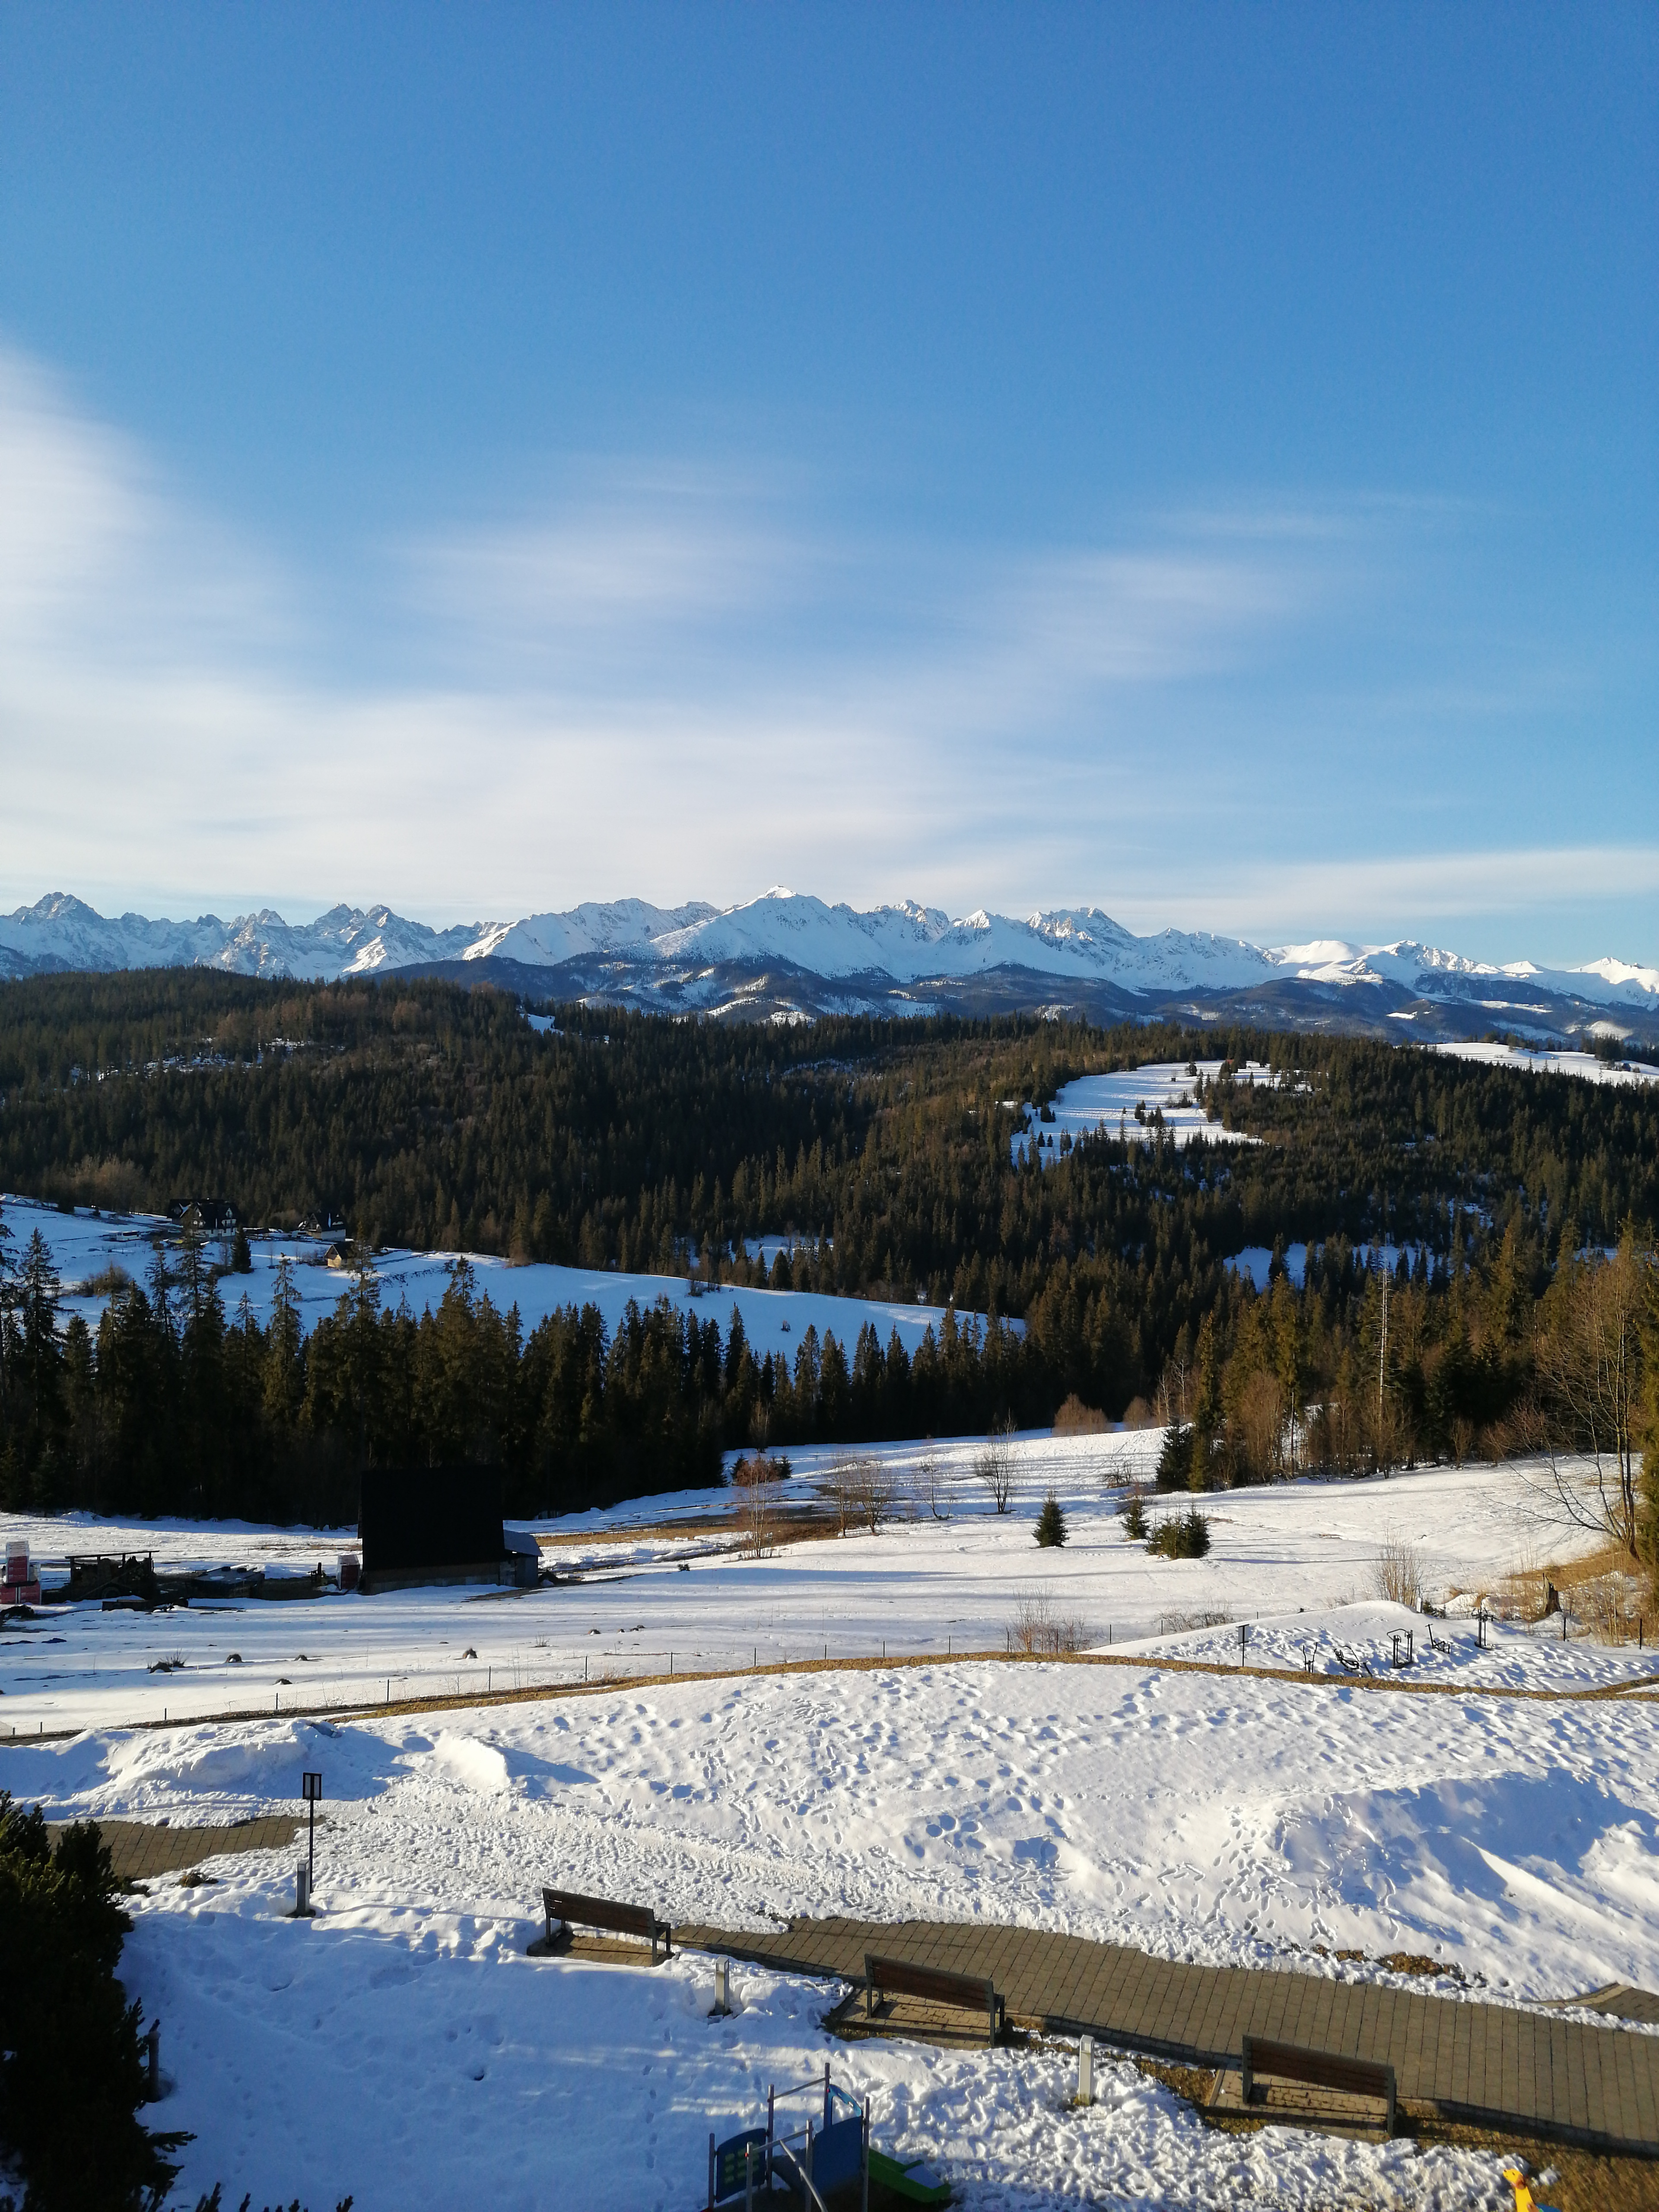
\includegraphics[width=0.45\linewidth]{img/image-2023-03-04_072211.jpg}
    \caption{Przykładowe zdjęcie gór i terenu zebrane w paśmie górskim Tatr.}
    \label{fig:example-static-terrain-photo}
\end{figure}

\begin{table}[!h]  \centering
\caption{Zebrane dane dotyczące przykładowego zdjęcia w paśmie górskim Tatr.}
\begin{tabular} {| c | c | c | c |} \hline
    Kąty widzenia (FoV) & \begin{tabular}[c]{@{}c@{}} Położenie \\ geograficzne \end{tabular}  & Kąty obrotu & Orientacja \\ \hline\hline
    
    \begin{tabular}[c]{@{}c@{}} $65,8946^\circ$ \\ $51,8465^\circ$ \end{tabular} & 
    
    \begin{tabular}[c]{@{}c@{}} $49,3393948$ N \\ $20,0812903$ E\\ $1006,09$ m n.p.m \end{tabular} & 
    
    \begin{tabular}[c]{@{}c@{}} $-167,37733^\circ$ \\ $1,7193204^\circ$ \\ $-0,98883315^\circ$ \end{tabular} & 
    
    Pionowa \\ \hline
   % \multicolumn{2}{|r|}{Suma:} & 123,45 \\ \hline
\end{tabular}
\label{tab:example-static-terrain-photo-data}
\end{table}

Wszelkie ilustracje oraz wizualizacje prezentowane w dalszej części pracy dyplomowej odnoszą się głównie do przedstawionego zdjęcia oraz parametrów zebranych podczas jego wykonywania. Przykładowo, rysunek w rozdziale \ref{sec:szczegoly_generowanie_modelu}, na którym prezentowany jest trójwymiarowy model terenu wygenerowany w ramach prototypu zawiera wizualizację widocznych na tym zdjęciu gór.

Na podstawie zebranych danych generowany był później trójwymiarowy model terenu. W~teorii wizualizował on przestrzeń zbliżoną do tej, która była widoczna z perspektywy obserwatora na wykonanym zdjęciu. Pozwalało to testować proces identyfikacji szczytów górskich symulując wejściowe klatki nagrań pochodzących z aparatu urządzenia.
\newpage

\section{Przegląd algorytmów i szczegóły implementacyjne}

Zaimplementowany w ramach platformy testowej proces rozpoznawania szczytów przebiega w podobny sposób, jak opisane w rozdziale \ref{section:teoretical_pipeline} podejście teoretyczne na podstawie analizy literaturowej. Na początku zbierane są dane z sensorów dotyczące kątów obrotu urządzenia oraz jego położenia GPS. Wykorzystując lokalizację określany jest współczynnik skalowania modelu związany ze zmianą wielkości pojedynczych kratek siatki terenu w zależności od szerokości geograficznej. Następnie generowany jest trójwymiarowy model ziemi z wykorzystaniem biblioteki OpenGL, a kamera ustawiana jest zgodnie z zebranymi danymi z czujników. Dla takiej wizualizacji określane są widoczne na niej szczyty górskie filtrując listę gór pochodzącą ze zbioru danych GeoNames. Zarówno dla wygenerowanej panoramy, jaki i wykonanego za pomocą aparatu urządzenia zdjęcia, wykrywane są krawędzie gór tworząc dwa obrazy binarne. Następnie wykorzystując metody dopasowania i sprawdzania podobieństwa między obrazami oraz listę widocznych wierzchołków na trójwymiarowym modelu stwierdzana zostaje ich widoczność na zdjęciu rzeczywistym. Odbywa się to~na~wygenerowanych obrazach binarnych, z których pobiera się odpowiedni wycinek w~zależności od~badanego szczytu. Dla tych gór, dla których stwierdzone zostanie podobieństwo z~odpowiednio dużym prawdopodobieństwem poprawności nakładane są etykiety nazw na~zdjęcie wejściowe. Tak zmodyfikowany obraz zostaje wysłany na wyjście procesu, a finalnie wyświetlony użytkownikowi. W przypadku działania na urządzeniu mobilnym w czasie rzeczywistym cykl ten powtarzany jest dla każdej kolejnej klatki nagrania zarejestrowanego na żywo. Diagram przedstawiający ten proces przedstawiono na rysunku \ref{fig:practical-pipeline}. Względem diagramu teoretycznego rozszerzony został on o dane pochodzące z sensorów oraz wykorzystanie aparatu urządzenia do pobrania kolejnych klatek obrazu.

\vspace{3em}

\begin{figure}[!h]
    \centering \includegraphics[width=1.0\linewidth]{img/flowchart_cale.drawio.png}
    \caption{Przepływ danych i sterowania procesu identyfikacji szczytów górskich z uwzględnieniem sensorów i urządzeń.}
    \label{fig:practical-pipeline}
\end{figure}


\subsection{Generowanie trójwymiarowego modelu terenu} \label{sec:szczegoly_generowanie_modelu}

Dane SRTM zapisane są w plikach jako ciąg wartości posortowanych zachód-wschód oraz północ-południe, które w ramach implementacji platformy testowej konwertowane są do postaci tablicy dwuwymiarowej. Numery rzędów i kolumn odpowiadają kolejno szerokości i długości geograficznej danego punktu, a wartości w poszczególnych komórkach tabeli to wysokość nad poziomem morza w danym miejscu. Takie przeskalowane ,,trójki'' (rząd, kolumna, wartość) odpowiadają współrzędnym trójwymiarowym OpenGL, a~w praktyce tworzą poszczególne wierzchołki modelu. W OpenGL prymitywy tworzy się z~siatki trójkątów i w ten sam sposób generowana jest mapa terenu w projekcie - trójkąty zostają utworzone z~kolejnych trzech posortowanych wierzchołków. Wizualizacja takiej siatki dla danych SRTM pokazana jest na rysunku \ref{fig:siatka}. Numerowane punkty odpowiadają kolejnym wartościom zapisanym w~tym zbiorze. 


\begin{figure}[!h]
    \centering \includegraphics[width=0.5\linewidth]{img/siatka.png}
    \caption{Wizualizacja tworzenia siatki trójkątów między punktami ze zbioru SRTM.}
    \label{fig:siatka}
\end{figure}

Dla tak stworzonych prymitywów dodawane jest cieniowanie zależne od położenia światła oraz wysokości poszczególnych punktów. Wymaga to obliczenia wektorów normalnych dla każdego wierzchołka. Uzyskuje się to poprzez normalizację sumy takich wektorów wszystkich trójkątów, w których skład wchodzi dany wierzchołek (wierzchołek częściowo opisuje od dwóch do sześciu trójkątów). Dzięki temu możemy w łatwy sposób kolorować i cieniować teren, co ma wpływ na detekcję krawędzi w dalszej części projektu, a także na poprawę walorów wizualnych przy ewentualnym podglądzie modelu.

Przykładowa wizualizacja trójwymiarowego terenu pokazano na rysunku \ref{fig:rendered}. Przedstawia ona wygenerowany model z ustawieniami lokalizacji i kątów obrotu odpowiadającym perspektywie zdjęcia \ref{fig:example-static-terrain-photo}. 

\begin{figure}[!h]
    \centering \includegraphics[width=0.45\linewidth]{img/rendered_scene.png}
    \caption{Przykład wizualizacji terenu z wykorzystaniem interfejsu OpenGL i danych SRTM.}
    \label{fig:rendered}
\end{figure}


\subsection{Widoczność szczytów górskich na trójwymiarowym modelu terenu} \label{sec:widocznosc_model}

Na model trójwymiarowy nanoszone są dane dotyczące szczytów górskich uzyskane ze~zbioru danych GeoNames. Zawierają one szerokość i długość geograficzną oraz wysokość nad poziomem morza dla każdego szczytu, które są przeliczane na odpowiadające położenie w~przestrzeni wygenerowanego terenu. Następnie, uzyskane w ten sposób wartości mapowane są na konkretny wierzchołek modelu. Tak przygotowane dane tworzą listę potencjalnie widocznych na zdjęciu wejściowym szczytów górskich. Ze względu jednak na to, że niektóre z~nich nie są widoczne na wizualizacji z perspektywy obserwatora musi zostać ona przefiltrowana.

Z tego powodu, na podstawie znajomości zagadnienia grafiki trójwymiarowej przez autora, został zaproponowany prosty, dwuetapowy proces filtracji listy potencjalnie widocznych wierzchołków. Oba kroki bazują na przystosowanych na potrzeby projektu metodach optymalizacji procesu renderingu poprzez usuwanie powierzchni niewidocznych. Jeśli potraktujemy szczyty górskie jako prymitywy i obiekty w generowanej scenie, to wykorzystanie takich algorytmów do określania ich widoczności wydaje się w pełni logiczne i uzasadnione. W~pierwszym etapie sprawdzane jest położenie poszczególnych punktów względem przestrzeni widzenia kamery. Następnie weryfikowana jest widoczność danego wierzchołka w kontekście bycia zasłanianym przez inne elementy terenu. Po przejściu tego procesu stwierdzana jest widoczność poszczególnych szczytów na wygenerowanym modelu.

\subsubsection{Filtracja szczytów poza polem widzenia kamery} \label{sec:frustum}

Pierwszym etapem filtrowania szczytów jest \textit{Frustum Culling} \cite{frutsum_culling}. Algorytm ten jest jedną z najpopularniejszych metod wykorzystywanych w grafice trójwymiarowej, której celem jest określenie wierzchołków znajdujących się w polu widzenia kamery. Dzięki temu pozwala usunąć obiekty, które nie znajdują się w zasięgu wzroku obserwatora. Polega on na projekcji współrzędnych trójwymiarowych na płaszczyznę dwuwymiarową obrazu. Na podstawie położenia kamery, kątów widzenia, kierunku patrzenia oraz innych, specyficznych dla danego rodzaju projekcji atrybutach tworzona jest matryca \textit{MVP} (z ang. Model View Projection \cite{MVP_matrices}). Opisuje ona przestrzeń widoczną dla kamery, a wizualnie charakteryzuje ostrosłup lub stożek ścięty. Przykładową wizualizację bryły widoczności dla projekcji perspektywicznej pokazano na rys. \ref{fig:frutsum-test}. Widoczne na niej obiekty w zacienionej przestrzeni - zielone koło - są odwzorowywane na obrazie, natomiast reszta jest usuwana - czerwone koła. Jeśli dany wierzchołek po przekształceniach z wykorzystaniem macierzy MVP ma prawidłowe współrzędne dwuwymiarowe - znajdujące się w zakresie szerokości i~wysokości tworzonego obrazu - to jest on widoczny dla obserwatora. 

\begin{figure}[!h]
    \centering \includegraphics[width=0.95\linewidth]{img/frutsum_test.png}
    \caption{Wizualizacja frustum culling. Ilustracja stożka widoczności kamery przy projekcji perspektywicznej. Odwzorowane zostaną tylko obiekty znajdujące się w przestrzeni stożka ściętego - zacieniona część. Czerwone koła będące poza obszarem widzenia kamery zostaną odrzucone. }
    \label{fig:frutsum-test}
\end{figure}


\par

Technika ta jest powszechnie stosowana w renderingu trójwymiarowym do optymalizacji tego procesu, ponieważ pozwala zmniejszyć liczbę wierzchołków oraz obiektów, które muszą być przetworzone i narysowane w generowanej scenie.

Na potrzeby pracy dyplomowej algorytm frustum culling został zaadaptowany do celów filtracji szczytów górskich, które na pewno nie są widoczne z perspektywy obserwatora, niezależnie od wygenerowanego terenu. Pozwala to znacznie zredukować listę potencjalnie widocznych szczytów na obrazie. 


\subsubsection{Filtracja zasłanianych szczytów} \label{sec:occlusion}

Dla pozostałych szczytów, które znajdują się w przestrzeni widocznej dla kamery, przeprowadzany jest tzw. \textit{Occlusion Culling} \cite{occlusion_culling}. Jest to kolejna technika optymalizacji procesu renderingu trójwymiarowego, której celem również jest odrzucenie struktur, które nie są widoczne z pozycji obserwatora. W tym wypadku znajdują się one jednak w~stożku widoczności ale położone są za innymi obiektami, więc są przez nie przesłaniane. Powoduje to, że nie muszą być przetwarzane i rysowane. Najprostsza implementacja wykorzystuje \textit{test głębokości} charakteryzujący to, jak blisko kamery znajduje się dany punkt, a co za tym idzie czy zasłania inne piksele (takie, które uzyskują mniejszą wartość współczynnika głębokości). 

\begin{figure}[!h]
    \centering \includegraphics[width=0.80\linewidth]{img/occlusion_culling.png}
    \caption{Wizualizacja Occlusion Culling. Czerwone koło jest przesłaniane przez zielony prostokąt, więc zostaje usunięte z procesu renderingu.}
    \label{fig:occlusion-culling}
\end{figure}

\par

W ramach opracowywanego procesu identyfikacji gór na obrazie occlusion culling pozwala sprawdzić, które wierzchołki odpowiadające poszczególnym szczytom przechodzą test głębokości. Jeśli dana góra uzyska dodatni wynik takiej próby to jest ona widoczna i powinna zostać oznaczona na obrazie. Test ten przeprowadzany jest z wykorzystaniem bufora zapytań (ang. queries \cite{queries_opengl}) w OpenGL. Taki mechanizm pozwala sprawdzać wynik wykonania danego zapytania. W projekcie sprawdzany jest stan wierzchołków (\textit{GL\_SAMPLES\_PASSED}) po przeprowadzeniu testu głębokości. Dla każdego szczytu wykonywana jest kwerenda i zależnie od odpowiedzi może on zostać usunięty z~listy potencjalnych szczytów górskich.

\par

Uzyskana po tym etapie lista zawiera szczyty, które na pewno są widoczne z perspektywy obserwatora na wygenerowanym trójwymiarowym modelu terenu. Następnym elementem jest dopasowanie ich do widocznych na zdjęciu wejściowym gór.


\subsubsection{Przykładowy rezultat widoczności szczytów górskich na wygenerowanym modelu}

Na rysunku \ref{fig:render_annotated} przedstawiono wcześniej wygenerowany model terenu (rys. \ref{fig:rendered}) z~naniesionymi nazwami widocznych na nim szczytów górskich. Ich widoczność została stwierdzona przy wykorzystaniu wyżej opisanego procesu filtrowania listy potencjalnie widocznych gór. Ze względu na duże zagęszczenie szczytów w widocznym na modelu paśmie górskim, liczba wyświetlanych nazw została ograniczona celem poprawy czytelności.  Dodatkowo obraz został wykadrowany z powodu zajmowania dużej części obrazu przez niebo oraz nieistotne elementy terenu.

\begin{figure}[!h]
    \centering \includegraphics[width=0.75\linewidth]{img/render_annotated.png}
    \caption{Przykładowy rezultat identyfikacji szczytów górskich na trójwymiarowym modelu terenu.}
    \label{fig:render_annotated}
\end{figure}


\subsection{Wyznaczanie odległości między dwoma punktami geograficznymi}

Jednym z obliczeń wykonywanych w trakcie procesu identyfikacji szczytów górskich wykonywanego na platformie testowej jest wyznaczanie odległości między dwoma punktami geograficznymi. Wyniki takich działań wykorzystywane są do ustalania odpowiedniej skali modelu trójwymiarowego względem rzeczywistości, ale również do wyliczenia odległości między obserwatorem, a widocznymi szczytami. Dlatego istotne było wybranie odpowiedniego algorytmu, który przy małej złożoności obliczeniowej będzie osiągać niski błąd. Przybliżone w następnym podrozdziale algorytmy były testowane w dalszej części pracy dyplomowej.

\subsubsection{Przegląd wybranych algorytmów}

W literaturze dostępnych jest wiele metod służących do obliczenia odległości między dwoma położeniami geograficznymi. Niektóre z nich wykorzystują elementy przybliżenia lub traktują kule ziemską jako inne figury trójwymiarowe, np. sferę lub walec. Na potrzeby pracy dyplomowej przybliżone zostały cztery algorytmy: sferyczne prawo cosinusów, metoda Haversiana, przybliżenie walcowe i iteracyjny algorytm Vincenta.

We wzorach poniżej występują następujące oznaczenia:

\begin{itemize}
    \item \textbf{d} - odległość między dwoma punktami geograficznymi.
    \item \textbf{R} - promień ziemi. Ze względu na różnicę pomiędzy promieniem równikowym i~biegunowym w projekcie wykorzystywany jest średni promień ziemi o długości $R=6371,0$~km \cite{promien_ziemi}.
    \item  \textbf{lat\textsubscript{i}} - (ang. latitude) szerokość geograficzna punktu \textit{i}
    \item  \textbf{long\textsubscript{i}} - (ang. longitude) wysokość geograficzna punktu \textit{i}
\end{itemize}



\paragraph{Sferyczne Prawo Cosinusów.} Jednym z podstawowych praw trygonometrii sferycznej jest \textit{Sferyczne Prawo Cosinusów} (ang. Spherical Law of Cosines). \cite{distance_geo} Jest to odpowiednik Prawa Cosinusów z geometrii płaskiej. Wykorzystywane jest do obliczania odległości między dwoma punktami na powierzchni sfery. Przy pomocy tej metody można uzyskać wynik charakteryzujący się dużą dokładnością, nawet przy małych odległościach.

\begin{align*}
    d=R * \arccos{(\sin{lat_{1}} * \sin{lat_{2}} + \cos{lat_{1}} * \cos{lat_{2}} * \cos{(long_{2} - long_{1}}))}
\end{align*}


\paragraph{Haversian.} Metoda \textit{Haversian} \cite{haversine,distance_geo} jest jedną z najczęściej wybieranych przy projektowaniu aplikacji wykorzystujących GPS czy bazujących na modelu ziemi. Została oparta na trygonometrii sferycznej jako jej uogólnienie. Pierwsze tabele haversianów były opisywane już na początku $XIX$ wieku, ale termin ten został sprecyzowany i opisany dopiero przez James'a Inmana w $1835$ roku.

\begin{align*}
    d=R * 2,0 * atan2(\sqrt{a}, \sqrt{1,0 - a})
\end{align*}
gdzie $a$ dane jest wzorem:
\begin{align*} \label{eq:formula}
\begin{gathered}
a = \sin{((lat_{2} - lat_{1})/2,0)}^{2} \\
    + \cos{lat_{1}} * \cos{lat_{2}} * \sin{((lat_{2} - lat{1}) / 2,0)}* \sin{((long_{2} - long_{1})/2,0)} 
\end{gathered}
\end{align*}

\paragraph{Przybliżenie walcowe równoodległościowe.} Następną z zaprezentowanych metod jest \textit{Przybliżenie Walcowe Równoodległościowe} (ang. Equirectangular Approximation). \cite{distance_geo} Algorytm ten opiera się na uproszczeniu, że Ziemia jest idealną sferą i traktuje ją jako płaszczyznę walcową. Sprawia to, że punkty o równej odległości względem równika na kuli ziemskiej są również tak samo odległe od równika na mapie. Dzięki takim założeniom zmniejszona zostaje złożoność obliczeniowa. Z tego powodu metoda ta jest często stosowana przy ograniczonych zasobach sprzętowych, na przykład w systemach wbudowanych.

\begin{align*}
d=R * \sqrt{((long_{2} - long_{1})*\cos{((lat_{1} + lat_{2})/2,0)})^{2} + (lat_{2}-lat_{1})^{2}}
\end{align*} 

\paragraph{Algorytm Vincenta.}
Ostatnim z opisywanych podejść jest iteracyjny algorytm Vincent'a. Jest to jedna z najbardziej zaawansowanych metod obliczania odległości geograficznej dająca bardzo dokładne rezultaty. Wadą tego rozwiązania jest duża złożoność, zarówno obliczeniowa jak i w kontekście opisu teoretycznego. Z tego powodu nie jest ona w pełni przybliżana w tej pracy dyplomowej. Dogłębnie opisana została w opracowaniu \cite{Vincenty}.



\subsection{Detekcja krawędzi gór} \label{sec:edge_detection}

Kolejnym etapem jest detekcja krawędzi na wygenerowanej panoramie oraz na rzeczywistym zdjęciu. Jest to istotny element procesu ze względu na to, że wyniki dla obu obrazów są do siebie porównywane, a następnie stwierdzana jest widoczność na nich poszczególnych szczytów.

\subsubsection{Oczekiwany rezultat} \label{sec:edge_detection_expected}

Wstępnie w ramach przeprowadzonych badań planowano wykrywać wszelkie krawędzie gór. Przykładowy oczekiwany rezultat zaprezentowano na rysunku \ref{fig:edge_detected_expected}. Jednak opracowanie odpowiedniej metody lub dobranie parametrów znanych algorytmów, tak by osiągnąć założony na początku cel okazało się niemożliwe w racjonalnej perspektywie czasu w kontekście tworzenie pracy dyplomowej magisterskiej, której tylko jednym z~elementów jest rozpoznawanie konturów. Głównym problemem było znalezienie uniwersalnego rozwiązania pozwalającego wykrywać w ten sposób krawędzie niezależnie od warunków pogodowych, jakości zdjęć czy innych zakłóceń.

\begin{figure}[!h]
    \centering \includegraphics[width=0.75\linewidth]{img/image-2023-03-04_072211_edge_expected_2.png}
    \caption{Przykład wstępnie oczekiwanego rezultatu detekcji krawędzi gór.}
    \label{fig:edge_detected_expected}
\end{figure}

Z tego względu zdecydowano się na ograniczenie detekcji krawędzi do najwyższych gór tworzących linię nieba. Jest to podejście podobne do opisanego w \cite{large-scale-visual}. Przykład wykrytych w ten sposób konturów pokazano na rysunku \ref{fig:edge_detected}. Konsekwencją takiego uproszczenia jest analiza jedynie szczytów górskich znajdujących się na tej linii oraz w bliskim jej sąsiedztwie ze względu na okno analizy o~pewnym rozmiarze. 



\begin{figure}[!h]
    \centering \includegraphics[width=0.75\linewidth]{img/image-2023-03-04_072211_edge.png}
    \caption{Przykład uproszczonej detekcji krawędzi gór.}
    \label{fig:edge_detected}
\end{figure}


Ma to szczególne znaczenie przy zdjęciach gór robionych z bliskiej odległości, gdy zajmują one dużą część obrazu w pionie oraz zawierają widoczne pasma górskie zróżnicowane pod względem wysokości. W takim przypadku efektem będzie pominięcie analizy wierzchołków znajdujących się w dolnej części zdjęcia, co finalnie oznacza niemożność ich identyfikacji. 

\subsubsection{Algorytm Canny} \label{sec:canny}

W ramach badań oraz platformy testowej, do celów detekcji krawędzi, zdecydowano się wybrać algorytm Canny \cite{Canny,SegmentationEdgeDetection,Canny_Opencv}. Mimo, że została opracowana w 1986 roku to dalej jest szeroko stosowaną metodą w przetwarzaniu cyfrowym obrazu rozwiązującą problem rozpoznawania konturów czy zmian w intensywności pikseli. Składa się ona z~czterech głównych etapów:

\begin{enumerate}
    \item \textbf{Usunięcie szumów.} Odbywa się to poprzez wygładzenie obrazu z wykorzystaniem filtru Gaussowskiego \cite{GaussianBlur} o rozmiarze jądra $5\textrm{x}5$. Pozwala to usunąć szum w postaci pojedynczych wyróżniających się pikseli. Efektem ubocznym jest bardziej rozmyte zdjęcie. 
    \item \textbf{Obliczenie siły i kierunek gradientu pikseli.} Na wygładzonym obrazie zastosowany zostaje operator Sobela \cite{Sobel} w pionie i poziomie celem określenia pierwszej pochodnej w obu tych kierunkach. Operator ten opiera się na splocie z macierzą $3\textrm{x}3$ wypełnioną wartościami zależnymi od orientacji. Następnie dla tych wyników oblicza się gradient oraz jego kierunek.
    \item \textbf{Tłumienie nie-maksymalne.} (ang. Non-maximum Suppression) \cite{Non-maximumSuppression} Polega na badaniu lokalnych maksimów dla znalezionych krawędzi. Dla piksela tworzącego dany kontur porównuje się go z wynikiem sąsiadów wzdłuż gradientu. Jeśli dany punkt jest lokalnym maksimum to uznawany jest za składową krawędzi. W innym przypadku jest odrzucany. Pozwala zachować piksele z najbardziej widoczną zmianą intensywności w danym otoczeniu.
    \item \textbf{Progowanie Histerezowe.} (ang. Hysteresis Thresholding) \cite{LectureComputerVision} Jest to filtrowanie krawędzi w zależności od siły gradientu. Opiera się na dwóch progach. Jeśli piksel znajduje się powyżej tych wartości to jest on uznawany za pewną (mocną) krawędź, natomiast jeśli poniżej to jest odrzucany. Piksele, których wartość gradientu znajduje się między progami zostają uznane za kontur w zależności od tego czy są połączone z~jakąś mocną krawędzią, czy nie.
\end{enumerate}

\vspace{5mm}

Parametry progowania histerezowego w implementacji platformy testowej zostały ustawione w taki sposób, żeby odrzucać głównie zaszumienie w części zdjęcia zawierającej niebo. Związane jest to z wcześniej opisanym problemem i decyzją o analizie jedynie najwyższych gór. Dla wynikowego obrazu binarnego wyszukuje się najwyższe krawędzie odrzucając te znajdujące się poniżej. Dlatego szum i dodatkowe wskazania w niższej części obrazu nie mają tak wielkiego znaczenia jak te na niebie, ponieważ nie są brane w~ogóle pod uwagę w trakcie analizy. Uzyskany efekt zawiera pojedynczy kontur w danej kolumnie zdjęcia tak jak na rysunku \ref{fig:edge_detected}. Taki sam schemat detekcji krawędzi stosowany jest w przypadku panoramy trójwymiarowego modelu terenu. W tym przypadku dobranie parametrów było dużo prostsze ze względu na stałe odwzorowanie kolorów takiego modelu. 

\subsection{Dopasowanie obrazów binarnych} \label{sec:dopasowanie}

Pomijając dodawanie nazw widocznych szczytów na zdjęciu rzeczywistym, dopasowanie obrazów binarnych celem stwierdzenia widoczności owych gór jest ostatnim etapem opracowywanego procesu ich identyfikacji. Wydaje się on również najważniejszym w~kontekście całego projektu, ponieważ to wyniki porównania ze sobą obrazów wygenerowanego modelu oraz faktycznego zdjęcia gór wpływają na odrzucenie lub etykietowane poszczególnych szczytów. Jeśli dany algorytm nie będzie w stanie dopasować do siebie badanych zdjęć z odpowiednio wysoką pewnością, szczyt może być niesłusznie uznany za niewidoczny, lub odwrotnie, niewidoczny szczyt jako widoczny. Z tego powodu, analiza tego zagadnienia oraz dostępnych algorytmów była bardziej dogłębna, a metody lepiej przetestowane.  



Operacja dopasowania obrazów zawierających krawędzie gór odbywa się na ich wycinkach o pewnym rozmiarze. W przypadku obrazu binarnego wyrenderowanego modelu centralnym punktem takiego fragmentu był piksel odpowiadający wierzchołkowi danego szczytu. Natomiast, dla zdjęcia wejściowego centrum było estymowane jako takie samo jak wizualizacji. Można przyjąć, że jest to miejsce hipotetycznego szczytu, gdyby wskazania sensorów urządzenia były idealne. Jednak ze względu, że w rzeczywistości takie mogą nie być, wycinek ten jest większy niż obrazu wygenerowanego terenu. Powiększony on jest o~pewną tolerancję, celem zwiększenia pewności zawierania się w nim widocznego szczytu. 

W poniższych podrozdziałach opisano dwie metody, które w ramach pracy dyplomowej były badane. Są to algorytmy oparte na dopasowaniu: wzorca (ang. template matching) oraz cech (ang. feature matching). Pierwsza z nich bada wartości pojedynczych pikseli, natomiast druga bierze pod uwagę kontekst poszczególnych punktów


\subsection{Dopasowanie na podstawie wzorca} \label{sec:template_matching}

Pierwszą z opisanych metod porównywania obrazów jest dopasowanie na podstawie wzorca (czasem określana także jako dopasowanie szablonu) \cite{template_opencv_1,template_opencv_2,template_adaptive,template_british,template_vidhya}. Do swojego działania wykorzystuje metody obliczania korelacji między dwoma zbiorami (w tym wypadku pikseli) dla każdego położenia. Dla danego położenia okna wynikiem takich obliczeń jest podobieństwo między dwoma obrazami. Finalnie, metoda ta zwraca najbardziej prawdopodobną lokalizację, w której szablon może znajdować się na zdjęciu wejściowym oraz jak pewne jest ich podobieństwo.

Ze względu na wykorzystanie jedynie numerycznych form porównania, metoda ta jest podatna na różne zniekształcenia między obrazami takie jak skalowanie czy rotacja, a~także na różnice w intensywności. Z tego względu może być efektywna przy porównywaniu prostych obrazów oraz przy kontrolowanych warunkach ich pozyskiwania. W kontekście porównywania obrazów binarnych zawierających kontury gór założenia te wydają się spełnione, co może przekładać się na lepsze wyniki \cite{feature_vs_template}.

Algorytmy oparte o analizę dopasowania wzorca tworzą tzw. mapę odpowiedzi lub mapę podobieństwa. Jest to dwuwymiarowa tablica o takich samych rozmiarach jak zdjęcie wejściowe, na którym szukany jest dany szablon. Wypełniania jest obliczonymi współczynnikami podobieństwa $R(x,y)$ dla każdego położenia wzorca względem głównego obrazu. Wykonywane jest to przesuwając szablonu po wszystkich pikselach obrazu wejściowego. Tak stworzona mapa zawiera w każdej komórce ustalony współczynnik dopasowania opisujący jak podobne są do siebie oba obrazy. Im wyższa jego wartość tym zdjęcia bardziej do siebie pasują. W przypadku wartości znormalizowanych pełną zgodność stwierdza się przy osiągnięciu wartości $1,0$ - obrazy są wtedy identyczne przy danym położeniu. Przykładowy wynik dopasowania wycinka wygenerowanego modelu trójwymiarowego do zdjęcia rzeczywistego w projekcie pokazany został na rysunku \ref{fig:template_matching_map}. Bardziej intensywny biały kolor na grafice oznacza wyższe wskaźnik podobieństwa między nimi (zakres wartości podobieństwa $0,0-1,0$ został przeskalowany na wartość pikseli $0-255$ w skali szarości). Na środku widoczny jest najbardziej jasny punkt - jest to najbardziej prawdopodobne położenie poszukiwanego szczytu. 


\begin{figure}[!h]
    \centering \includegraphics[width=0.6\linewidth]{img/template_matching_map.png}
    \caption{Przykład mapy podobieństwa uzyskanej wykorzystując algorytm dopasowania wzorca przy porównaniu obrazów binarnych krawędzi gór.}
    \label{fig:template_matching_map}
\end{figure}


W bibliotece OpenCV występują trzy metody obliczania wartości w mapie dopasowania: kwadrat różnicy (ang. Squared Difference - SQDIFF), korelacja krzyżowa (ang. Cross-correlation - CCORR), współczynik korelacji krzyżowej (ang. Cross-correlation coefficient - CCOEFF). Wszystkie z nich występują zarówno w wersji bez, jak i z normalizacją \cite{template_opencv_1}\cite{template_opencv_2} do zakresu wartości $0,0-1,0$. 

W trakcie prac badawczych wykorzystane zostały tylko metody oparte na korelacjach (CCORR i CCOEFF). Kwadrat różnicy został całkowicie pominięty z opisu teoretycznego oraz z porównań algorytmów z dalszej części pracy dyplomowej. Związane jest to z bardzo słabymi, bliskimi zeru, wynikami testów wstępnych. Dodatkowo, badania te pokazały przewagę wersji znormalizowanych korelacji krzyżowej i współczynnika korelacji, nad ich wersjami bez normalizacji. Związane to jest z łatwiejszym doborem parametrów przy ograniczonym zakresie wartości. Z tego powodu brane pod uwagę są tylko metody z~normalizacją. 

W opisanych poniżej równaniach stosowanych do wypełnienia mapy podobieństwa wykorzystywane są następujące oznaczenia:

\begin{itemize}
    \item $\textbf{R(x, y)}$ - wyliczony współczynnik podobieństwa wzorca i zdjęcia wejściowego przy położeniu okna  o środku $x, y$. Całościowo $R$ oznacza tzw. mapę odpowiedzi/podobieństwa zawierającą obliczony współczynnik w każdej lokalizacji.
    \item $\textbf{x, y}$ - współrzędne danego piksela zdjęcia wejściowego.
    \item $\textbf{x',y'}$ - współrzędne danego piksela wzorca.
    \item $\textbf{I(x, y)}$ - wartość/intensywność/jasność piksela zdjęcia wejściowego o danych współrzędnych.
    \item $\textbf{T(x',y')}$ - wartość/intensywność/jasność piksela wzorca o danych współrzędnych.
\end{itemize}



\paragraph{Znormalizowana korelacja krzyżowa.}
Metoda ta wykorzystuje korelację krzyżową jako metrykę podobieństwa. Mierzy ona dopasowanie szablonu i zdjęcia wejściowego dla każdej możliwej pozycji drugiego obrazu. W praktyce polega ona na przesuwaniu okna analizy po całym obrazie wejściowym i dla każdej takiej lokalizacji obliczany jest iloczyn skalarny wartości pikseli. Wyższa wartość korelacji wskazuje na większe podobieństwo między szablonem, a obszarem docelowym.

Wersja ta skupia się wyłącznie na korelacji punktowej. Z tego powodu jest ona skuteczna głównie w przypadku, gdy dopasowane obrazy mają podobny zakres jasności oraz minimalne zniekształcenia względem siebie takie jak rotacja czy skalowanie.

Wartości w mapie dopasowania, dla tej metody, obliczane są zgodnie z równaniem:

\begin{align*}
    R(x,y)= \frac{\sum_{x',y'} (T(x',y') \cdot I(x+x',y+y'))}{\sqrt{\sum_{x',y'}T(x',y')^2 \cdot \sum_{x',y'} I(x+x',y+y')^2}}
\end{align*}



\paragraph{Znormalizowany współczynnik korelacji.}
Metoda ta również wykorzystuje korelację krzyżową oraz iloczyn skalarny wartości pikseli. Stosuje ona dodatkowo normalizację uśredniającą jasności obrazu do zera. Z tego powodu w przeciwieństwie do poprzedniego rozwiązania nie skupia się wyłącznie na korelacji punktowej, ale również bierze pod uwagę różnice w intensywności pikseli w danym otoczeniu. Dzięki temu, wersja ta jest bardziej elastyczna i odporniejsza na zmianę warunków oświetleniowych czy kontrastu między zdjęciami oraz na różnego typu zniekształcenia.  

Miara podobieństwa opisana jest wzorem:

\begin{align*}
    R(x,y)= \frac{ \sum_{x',y'} (T'(x',y') \cdot I'(x+x',y+y')) }{ \sqrt{\sum_{x',y'}T'(x',y')^2 \cdot \sum_{x',y'} I'(x+x',y+y')^2} }
\end{align*}

gdzie $T'$ i $I'$ dane są wzorami:

\begin{align*}
    \begin{array}{c}
        T'(x',y')=T(x',y') - 1/(w \cdot h) \cdot \sum _{x'',y''} T(x'',y'') \\ 
        I'(x+x',y+y')=I(x+x',y+y') - 1/(w \cdot h) \cdot \sum _{x'',y''} I(x+x'',y+y'') 
    \end{array}
\end{align*}

$T'$ i $I'$ oznaczają wartość danego piksela, odpowiednio dla szablonu i zdjęciu wejściowego, poddaną normalizacji uśredniającej względem jasności otoczenia. Sprawia ona, że wskazania średnie w danym punkcie przyjmują wartość $0$. Natomiast pozostałe wyniki równania określają odległość wartości jasności pikseli od średniej.



\subsection{Dopasowanie na podstawie cech} \label{sec:feature_matching}

Drugą metodą detekcji podobieństwa między obrazami wykorzystywaną w projekcie pracy dyplomowej jest dopasowanie na podstawie cech (z ang. Feature Matching). Polega ona na porównywaniu między zdjęciami pewnych, charakterystycznych cech - stąd nazwa metody. Mogą być nimi m.in.: krawędzie, tekstury, nieszablonowe zmiany jasności czy elementy wyróżniające się w danej przestrzeni. Na ich podstawie, wyszukując podobne struktury na obu zdjęciach, stwierdza się ich podobieństwo \cite{opencv_understand_features}\cite{feature_lieberman}. 

Metoda ta jest jedną z częściej wykorzystywanych w procesie tzw. rejestracji zdjęć (ang. Image Registration) lub inaczej nazywane wyrównaniem zdjęć (ang. Image Alignment) \cite{szelinski}. Są to techniki mające na celu zarejestrować i wyrównać obrazy zawierające tę samą scenę lub obiekt ale z różnych punktów widzenia czy w różnych warunkach oświetleniowych~\cite{image_reg_geeks,image_reg_pyimage}. Pozwalają one uzyskać dla nich jednolity układ współrzędnych, przeprowadzić korekcję zniekształceń, tworzyć z wielu zdjęć panoramę lub zdjęcia trójwymiarowe, a~także, co istotne w kontekście pracy dyplomowej, porównywać obrazy. Z~powodzeniem jednak rejestrowanie zdjęć wykorzystywane jest również w przetwarzaniu dokumentów czy śledzeniu obiektów na nagraniach \cite{image_reg_practical}. 

W teorii, feature matching jest bardziej elastyczny niż metoda oparta na szablonach oraz bardziej odporna na zniekształcenia, rotacje czy skalowanie. Daje ona dobre wyniki przy skomplikowanych scenach bogatych w unikalne cechy, ze zmiennymi widokami oraz przy poszukiwaniu złożonych struktur o nietrywialnych elementach. Jednocześnie radzi sobie gorzej z prostymi scenami, w szczególności podczas wyszukiwania konkretnego wzoru lub prymitywnych obiektów o ograniczonej możliwości transformacji. Z tego powodu może się okazać mało skuteczna przy porównywaniu obrazów binarnych krawędzi gór, które nie zawierają zbyt dużej liczby charakterystycznych cech, a jedynie zbiór białych linii na jednolitym tle.


Podejście to składa się z kilku etapów. Na początku wybierane są punkty charakterystyczne, zawierające pewnego rodzaju szczególne cechy. Określane są dla nich również deskryptory opisujące wybrane ich właściwości. Odbywa się to dla zdjęć wejściowych: poszukiwanego oraz przeszukiwanego. Następnie porównuje się punkty z obu obrazów, dopasowując do siebie te z największym podobieństwem. Ze względu na możliwe szumy i~błędne przyporządkowania, należy je odpowiednio przefiltrować i odrzucić niepoprawne. Ostatnim krokiem jest przekształcenie szablonu na podstawie dopasowanych punktów kluczowych, w taki sposób by poprawnie określić miejsce szukanego obiektu na drugim obrazie. 



\subsubsection{Punkty kluczowe i ich deskryptory} \label{sec:feature_matching_keypoints}

Pierwszym etapem dopasowania obrazów na podstawie cech jest wyszukanie punktów kluczowych oraz ich deskryptorów \cite{affine_point}\cite{feature_cornell}. Są one podstawą działania tego rodzaju algorytmów, ponieważ są ze sobą porównywane w celu stwierdzenia podobieństwa danych elementów zdjęć.

Punkty charakterystyczne określają specyficzne lub wyjątkowe obszary na zdjęciu, sklasyfikowane na podstawie wyróżnionych unikalnych cech. Z tego względu mogą być jednoznacznie identyfikowane w różnych widokach, a nawet na różnych zdjęciach. Ich obszary mogą być specyficzne ze względu na różne atrybuty, takie jak: wzór, tekstura, strukturę jaką tworzą lub poprzez krawędzie i kąty. Dany punkt by mógł zostać uznany za kluczowy musi spełniać określone niezmienniki, tzn. musi być niezależny od transformacji takich jak skalowanie, rotacja, zmiany jasności czy perspektywy. Kolejnym założeniem odnoszącym się do punktów kluczowych jest powtarzalność. Musi być możliwość identyfikacji tych samych cech na kolejnych scenach lub obrazach. Wizualizację wykrytych na obrazie binarnym punktów charakterystycznych wraz z ich kierunkiem oraz rozmiarem pokazano na rysunku \ref{fig:feature_keypoints}.

\begin{figure}[!h]
    \centering \includegraphics[width=0.6\linewidth]{img/keypoints.png}
    \caption{Przykład części wykrytych punktów charakterystycznych wraz z ich kierunkiem i~rozmiarem na obrazie binarnym krawędzi gór.}
    \label{fig:feature_keypoints}
\end{figure}


Cechy punktów kluczowych opisywane są przez tak zwane deskryptory tworzone dla każdego miejsca charakterystycznego. Zawierają głównie informację na temat otoczenia danego punktu. Opisują intensywność pikseli, kierunek ewentualnych gradientów, wzór, który tworzy czy jego histogram. Zestaw tych cech jest niezależny od lokalizacji, dzięki czemu pozostałe fragmenty obrazu nie mają na niego wpływu i może być porównywany między różnymi scenami. Deskryptory najczęściej przybierają formy wektorowe. 

\paragraph{SIFT.} Przykładem algorytmu pozwalającego na wyszukiwanie opisanych punktów i cech jest SIFT (z ang. Scale-Invariant Feautre Transform) \cite{SIFT}\cite{SIFT_opencv}. Składa się on z kilku etapów. Pierwszym jest poszukiwanie potencjalnych punktów kluczowych poprzez zastosowanie techniki \textit{Różnicy Gaussów} (ang. Difference of Gaussian). Jest to technika nakładania filtrów gaussa o dwóch rozmiarach okna, a następnie obliczaniu różnicy wartości pikseli między nimi. Celem tego jest wyszukanie punktów niezależnych od skalowania. Wyszukując ich ekstrema uzyskuje się wstępną listę punktów charakterystycznych o różnych rozmiarach. Kolejnym etapem jest ich filtracja ze względu na kontrast (niski kontrast może oznaczać wrażliwość na szum) lub odrzucając mniej istotne krawędzie. Wykonywane jest to na podstawie progowania o pewnym ustalonym progu dla lokalnych ekstremów. Pozostałe punkty charakterystyczne traktowane są jako stabilne i wartościowe. Następnie dla każdego z nich określany jest kierunek oraz rozmiar, w zależności od jego sąsiedztwa. Pozwala to uodpornić algorytm na zmiany rotacji względem kolejnych scen. Na końcu obliczane są deskryptory cech okolicy danego punktu.



\paragraph{ORB.} Drugą z opisywanych metod służących do określania punktów charakterystycznych oraz ich deskryptorów jest ORB (z ang. Oriented FAST and Rotated BRIEF) \cite{ORB}\cite{ORB_opencv}. Jest to połączenie algorytmów FAST (z ang. Features from Accelerated Segment Test \cite{fast}) do wykrywania punktów kluczowych oraz BRIEF (z ang. Binary Robust Independent Elementary Features \cite{brief}) do opisu cech. Ze względu na jej hipotetyczną wydajność autor artykułu, w którym opisuje tę metodę, zatytułował go \textit{ORB: Efektywna alternatywa dla SIFT oraz SURF} (oryg. \textit{ORB: An effective alternative to SURF and SIFT} \cite{ORB}). Nazwa ta związana jest z mniejszą złożonością obliczeniową, a co za tym idzie krótszym czasem wykonania. Odnosi się również do patentów, którymi były objęte oba algorytmy. W przeciwieństwie do nich, ORB od razu był wolny od takich ograniczeń (SIFT był opatentowany w momencie powstania tamtego artykułu, lecz licencja ta wygasła w marcu 2020 r.). Ze względu, że FAST nie był odporny na obroty scen, w algorytmie ORB obliczana jest orientacja punktów, opisywana w formie kołowej. Modyfikuje on również metodę BRIEF wykorzystując obliczoną wcześniej rotację. Tworzone są na ich podstawie macierze obrotu, służące do nadawania deskryptorom kierunku. Ma to na celu zniwelowanie problemów algorytmu BRIEF z wydajnością. Dzieje się to jednak kosztem utraty wysokiej wariancji oraz nieskorelowania punktów. By odzyskać te cechy ORB przeprowadza zachłanne przeszukiwanie potencjalnych wartości wynajdując takie, które posiadają te właściwości. 



\subsubsection{Dopasowanie punktów kluczowych obu zdjęć} \label{sec:feature_matching_matching}

Obliczone punkty charakterystyczne oraz ich deskryptory dla obu zdjęć należy ze sobą porównać i przyporządkować do siebie najbardziej pasujące tworząc pary. Wykonywane jest to poprzez zestawienie ze sobą poszczególnych cech z obu zdjęć. Popularnymi metodami porównywania punktów kluczowych oraz deskryptorów są na przykład: algorytm siłowy (ang. Brute Matching) lub FLANN (z ang. Fast Library for Approximate Nearest Neighbors) \cite{opencv_matching}\cite{feature_unik}.

Jak wszelkiego rodzaju algorytmy siłowe, tak i w tym przypadku polega on na przeszukiwaniu przestrzeni rozwiązania poprzez sprawdzenie wszystkich możliwych kombinacji i wybraniu najlepszych. Dany punkt charakterystyczny z dopasowywanego szablonu porównuje się z każdym punktem ze zdjęcia, na którym poszukujemy interesujący nas obiekt. Na podstawie takich porównań tworzy się pary o największym podobieństwie. Zaletą takiego rozwiązania jest gwarancja uzyskania rezultatów optymalnych z najlepszymi dopasowaniami. Wadą podejścia opartego na metodach siłowych jest natomiast długi czasu wykonania oraz wykorzystanie większych zasobów pamięciowych. Złożoność obliczeniowa tego algorytmu wynosi $O(n^2)$.

FLANN \cite{FLANN} \cite{FLANN_manual} zorientowany jest na szybkie znajdowanie najbliższych sąsiadów. W~praktyce nie jest to jedna metoda, a zbiór algorytmów służących do tego celu. W zależności od użytych parametrów takich jak sposób indeksowania, liczba epok, wymagana dokładność czy preferowana metoda możliwe jest uzyskanie różnych rezultatów. W cytowanej dokumentacji FLANN zasugerowane są optymalne ustawienia dla wybranych algorytmów wyszukujących punkty charakterystyczne, w tym dla opisanych w poprzednim podrozdziale ORB i SIFT. Zgodnie z założeniem mają być to szybkie rozwiązania, a~osiągane jest to kosztem znajdowania tylko przybliżonego rozwiązania. Z tego względu może on dawać mniej dokładne wyniki niż na przykład metoda siłowa. W tym przypadku, średnia złożoność obliczeniowa jest na poziomie $O(\log(n))$, co ma znaczenie przy dużych zbiorach danych. 

Przy obu podejściach, możliwe jest uzyskanie dla każdego punktu $k$ najbliższych sąsiadów (w przypadku metody siłowej $k$ najlepszych). Ze względu na liczbę punktów charakterystycznych oraz wartość ich dopasowania zasadnym staje się wybór tylko pewnej ich części w zależności od przyjętego kryterium. W projekcie magisterskim, jeśli dopasowywany jest tylko jeden punkt wykorzystywana jest filtracja za pomocą progowania podobieństwa. W przypadku $k\geq2$ wykorzystywany jest tzw. test współczynników. Określa on jak bardzo lepsze musi być pierwsze z $k$ dopasowań w porównaniu do pozostałych, by para mogła być uznana za wartościową. Jeśli przykładowo pierwszy i drugi mają porównywalną wartość podobieństwa to dopasowania dla tego punktu zostają odrzucone. 

Na rysunku \ref{fig:matched_points} przedstawiono przykład dopasowanych punktów kluczowych dla krawędzi gór wygenerowanego modelu oraz rzeczywistego zdjęcia. Do celów wizualizacyjnych zostało wybrane $10$ dopasowań o najwyższym współczynniku podobieństwa, celem zwiększenia przejrzystości.

\begin{figure}[!h]
    \centering \includegraphics[width=0.7\linewidth]{img/matched_points.png}
    \caption{Przykład dopasowanych punktów kluczowych dwóch obrazów binarnych krawędzi gór.}
    \label{fig:matched_points}
\end{figure}

\subsubsection{Projekcja położenia z wykorzystaniem homografii} \label{sec:feature_matching_homography}

Rozłożenie połączonych punktów może tworzyć nieregularne kształty. Z tego powodu dopasowanie szablonu na zdjęciu rzeczywistym z odpowiednią skalą, rotacją i zniekształceniami jedynie na podstawie tych połączeń może być wizualnie trudnym zadaniem. Do tego celu może być wykorzystana estymacja z wykorzystaniem transformacji homograficznej \cite{homography_aids}. 

Homografia opisuje relacje płaską między dwoma obrazami z różnych punktów obserwacji. Reprezentowana jest poprzez macierz $3\textrm{x}3$ z ośmioma punktami swobody, tworzącą tak zwaną macierz transformacji perspektywicznej. Ten rodzaj przekształcenia zachowuje proste, czteropunktowe kontury obrazu, ale pozwala na deformacje obrazu bez zachowania sztywności elementów. Przy jej użyciu możliwa jest projekcja pikseli na wybraną płaszczyznę \cite{homography_opencv_explain}\cite{homography_maulion}.


W kontekście porównania obrazów na podstawie cech technika ta pozwala na transformację szablonu względem dopasowanych punktów kluczowych. Wykonywane jest to w~taki sposób, że możliwe jest jego nałożenie na obraz główny z jak najlepszym wyrównaniem i odwzorowaniem przekształceń. Pozwala to również na stwierdzenie dokładnego położenia szukanego fragmentu obrazu \cite{homography_opencv}. Przykład takiej transformacji z zaznaczeniem pewnej liczby punktów kluczowych oraz oznaczeniem szukanego obiektu pokazany został na rysunku \ref{fig:homography} (ze względu na małą przejrzystość takiej grafiki przy dopasowaniu krawędzi gór, do celów prezentacyjnych wykorzystany został prosty obiekt świata rzeczywistego). 


\begin{figure}[!h]
    \centering 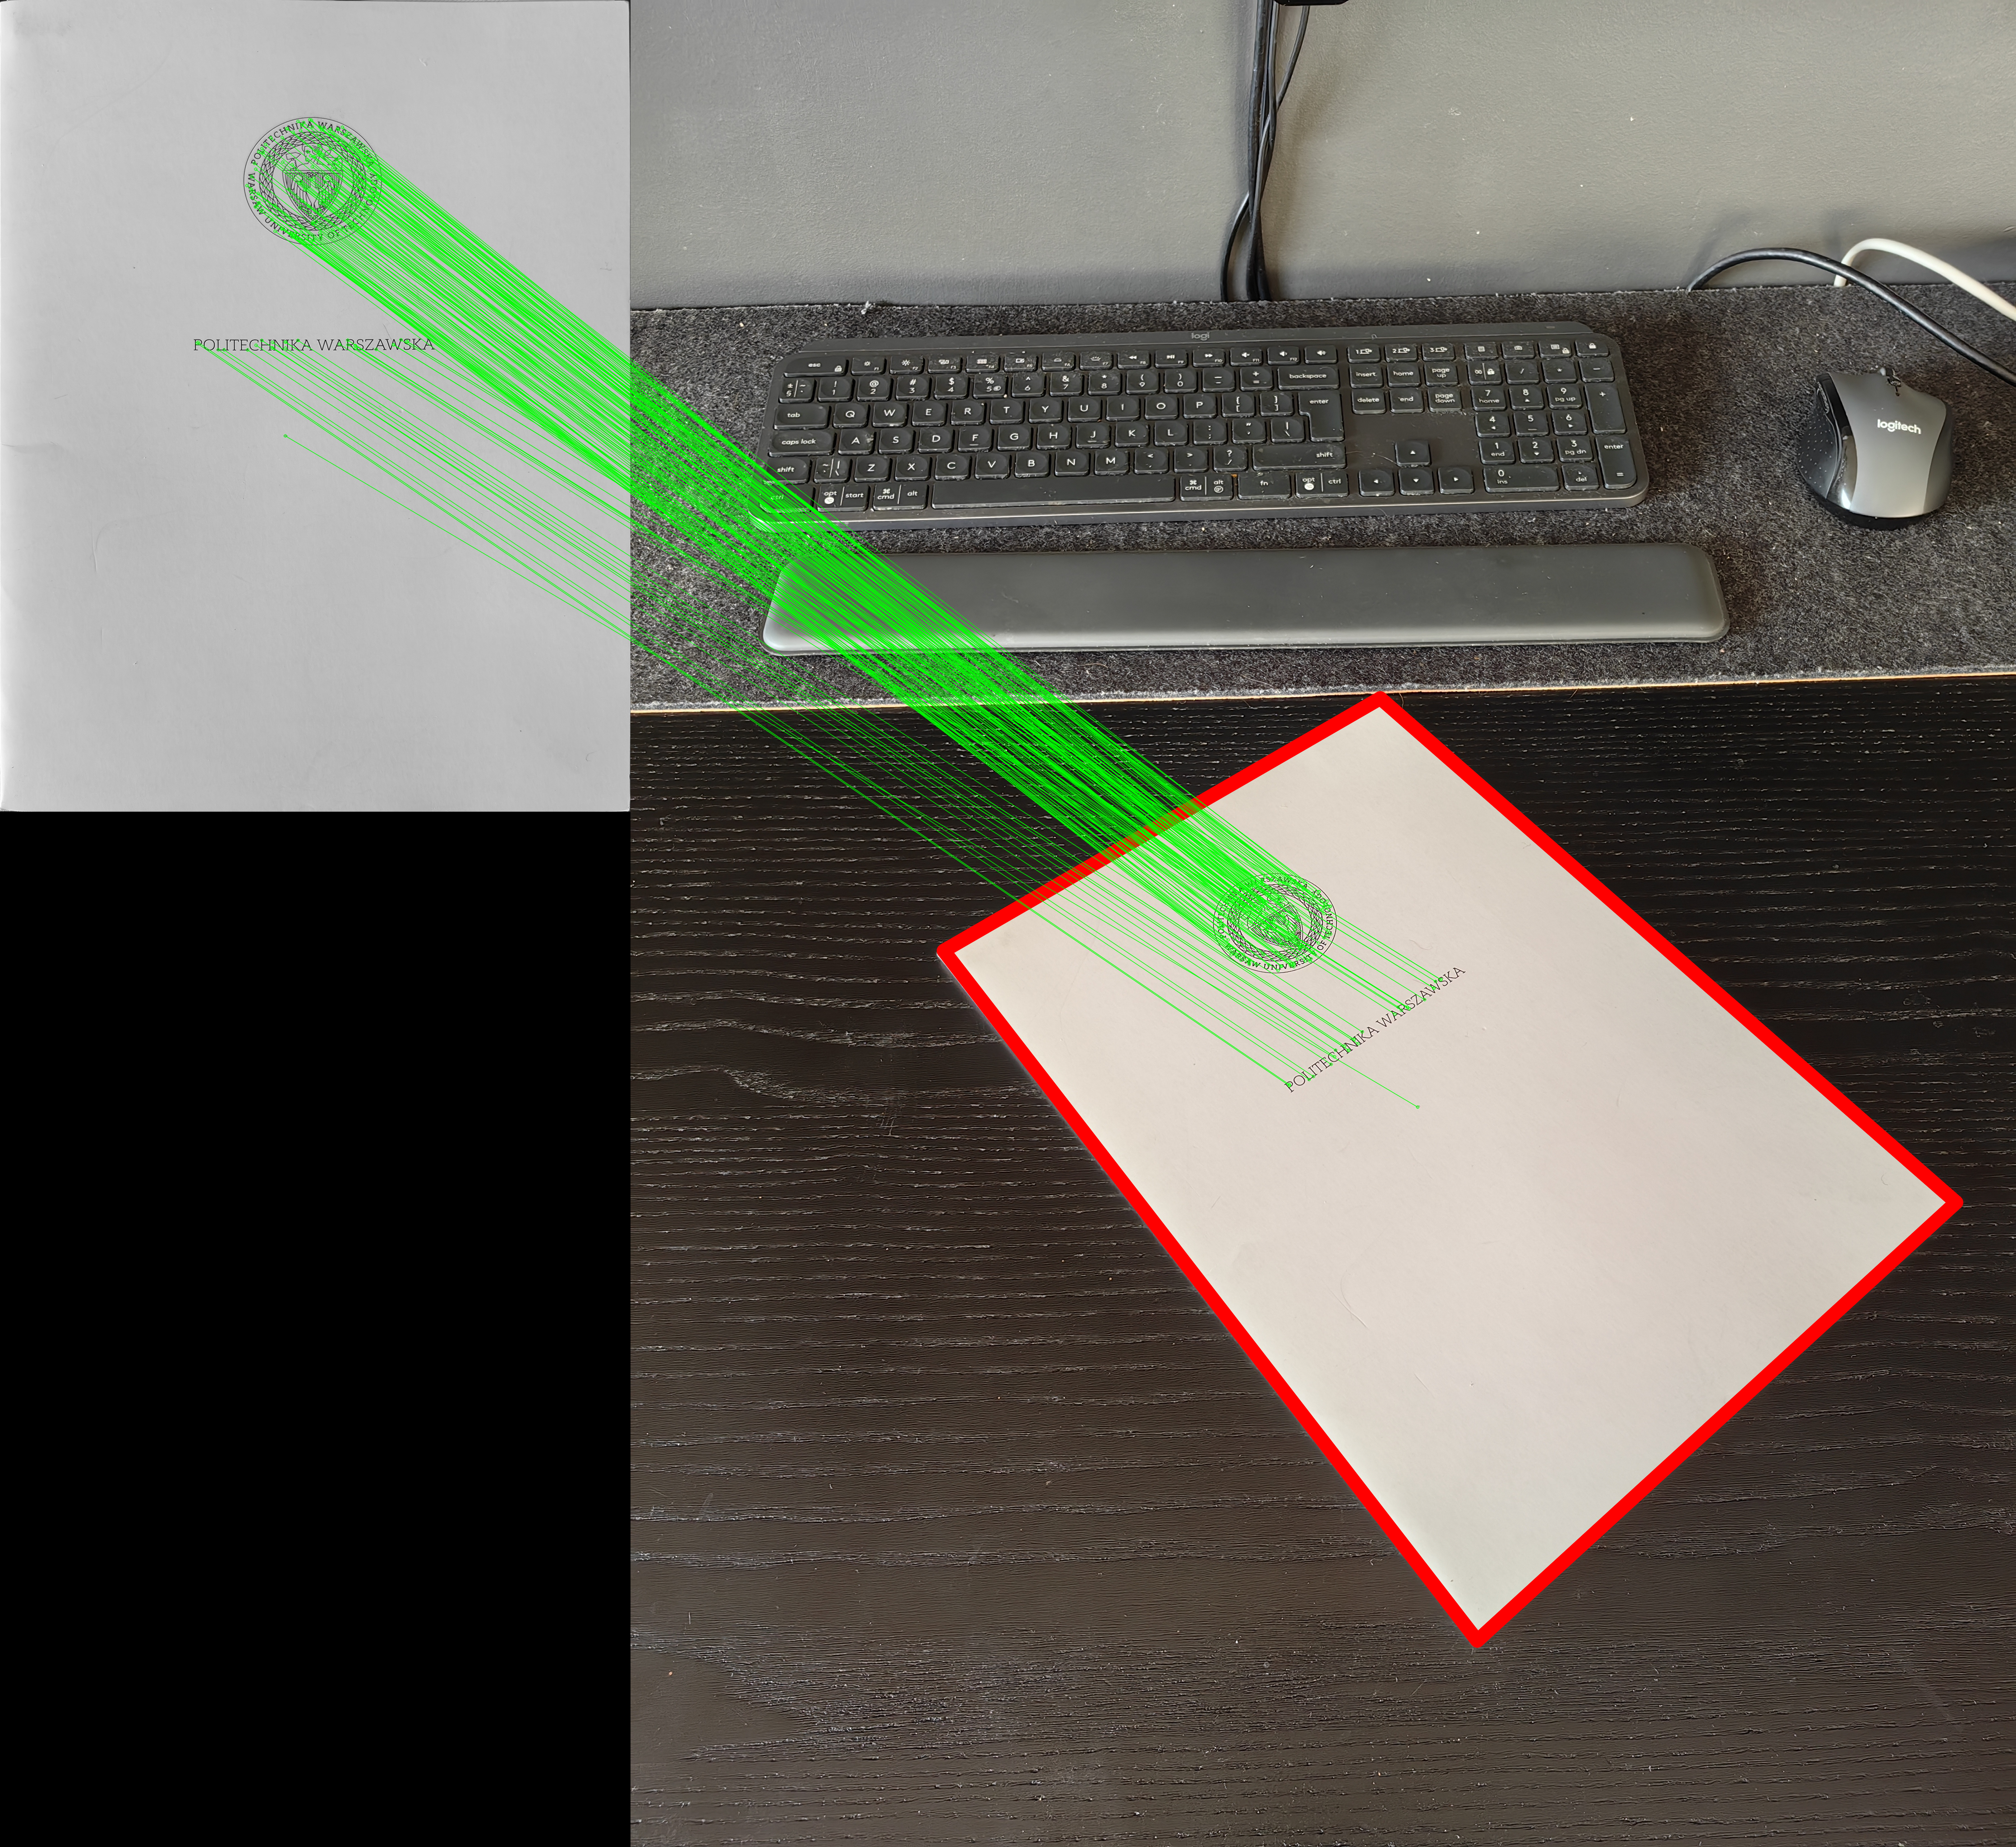
\includegraphics[width=0.65\linewidth]{img/homography.png}
    \caption{Przykład transformacji homograficznej na podstawie dopasowanych punktów kluczowych celem oznaczenia położenia szukanego szablonu.}
    \label{fig:homography}
\end{figure}

W części badawczej pracy dyplomowej do znalezienia optymalnej macierzy homografii wykorzystywane są dwie metody: RANSAC i PROSAC. Mają one za zadanie przeszukiwanie przestrzeni danych oraz obliczenie wartości tej macierzy. 

\paragraph{RANSAC.} Pierwszą z opisywanych metod wykorzystywanych do obliczenia macierzy homografii na podstawie punktów kluczowych jest RANSAC (z ang. Random Sample Consensus) \cite{ransac}. Jest to iteracyjny algorytm służący do estymowania wybranych parametrów na podstawie zestawu danych wejściowych. W przypadku feature matching jest to wyliczenie wartości macierzy transformacji homograficznej, gdy na wejściu zostaje przesłany zestaw punktów kluczowych. Jego celem jest znalezienie jak najlepszego modelu pasującego do jak największej części zbioru.

Algorytm ten według literatury jest skuteczny przy pracy z zaszumionymi danymi oraz ze zbiorami zawierającymi wiele wartości odstających. Wynika to z faktu, że skupia się on na znalezieniu modelu, który pasuje do jak największego zbioru będącego w pewnej odległości od siebie, ignorując przy tym wartości znacznie się różniące i odstające.

W trakcie danej iteracji metody RANSAC wykonywane są następujące kroki:

\begin{enumerate}
    \item Losowy wybór minimalnego zbioru danych potrzebnego do estymowania parametrów. W przypadku dopasowania obrazów zawsze są to co najmniej cztery punkty kluczowe.
    \item Na podstawie wybranego podzbioru obliczane są parametry modelu. W opisywanym kontekście są to wartości macierzy homografii.
    \item Stwierdzenie jaka część danych wykorzystując stworzony model mieści się w granicach ustalonej tolerancji. 
    \item Na podstawie danych będących w ustalanych granicach obliczana jest jakość wygenerowanego modelu. 
\end{enumerate}

Kroki te powtarza się przez określoną liczbę iteracji lub do znalezienia modelu o~wystarczająco wysokim wskaźniku jakości. W pierwszym przypadku wybierany jest ten model ze wszystkich wygenerowanych, dla którego największy podzbiór danych spełnia założone dopasowanie. 


\paragraph{PROSAC.} Kolejnym prezentowanym rozwiązaniem jest PROSAC (ang. Progressive Sample Consensus) \cite{prosac}. Jest to rozwinięcie algorytmu RANSAC poprzez zmianę sposobu wyboru podzbioru danych. W pierwszym z opisywanych podejść jest to wykonywane przez losowy wybór próbek. Natomiast, w przypadku algorytmu PROSAC próbkowanie to odbywa się metodą progresywną na podstawie wyników z poprzednich iteracji. Biorąc pod uwagę oceny ostatnich modeli, priorytezuje on te dane, które są bardziej prawdopodobne. Skupienie się na prawidłowych próbkach ma na celu zwiększenie szansy na szybsze znalezienie dobrego i wystarczającego modelu. Pozostałe kroki są takie same jak w RANSAC. Rozwiązanie to jest częściej wykorzystywane, gdy istnieje duża liczba wartości odstających w zbiorze danych oraz potrzebne jest szybsze dopasowanie modelu. 
\newpage

\section{Dodatkowe problemy implementacyjne}


\subsection{Niedokładność sensorów urządzeń}

Jednym z elementów procesu identyfikacji szczytów górskich na obrazie jest generowanie trójwymiarowego modelu terenu. W stworzonej platformie testowej opiera się on na interfejsie OpenGL i danych NTM. Moduł ten umożliwia kalibrację kamery zgodnie z ustawieniami danego urządzeniami.  Dzięki temu, generowany model może być łatwo porównywany z rzeczywistymi, statycznymi zdjęciami. Możliwe jest również ustawienie obserwatora w dowolnym miejscu, np. zgodnie z danymi dotyczącymi zarejestrowanego wcześniej obrazu z urządzenia mobilnego oraz obserwacja terenu z różnych perspektyw. 

Podczas testów wykorzystujących przygotowany zbiór statycznych zdjęć zauważono, że generowany model na podstawie zapisanych danych, w szczególności kątów obrotu, był w niektórych przypadkach przesunięty o pewną odległość względem zdjęcia rzeczywistego. Wynikało to przeważnie ze wskazań czujnika obrotów. Przesunięcia odpowiadały najczęściej błędom o wielkości $2^\circ-5^\circ$. Dzięki temu, w dalszej pozostałej części testowej pracy dyplomowej założono pewną tolerancję odpowiadającej takim niedokładnościom uzyskiwanych danych.

\subsection{Skalowanie trójwymiarowego modelu terenu}

Testowanie wizualizacji trójwymiarowej wykazało również błędne założenia na~temat skalowania terenu. Wstępnie wykorzystywane były ogólnie przyjęte przybliżenia jednej jednostki szerokości oraz długości geograficznej. Wygenerowana w ten sposób panorama terenów Tatr była rozciągnięta w poziomie względem tego co widoczne na~odpowiadających zdjęciach.

Na podstawie analizy tego problemu stwierdzono, że problem wynika ze zbyt dużej powierzchni generowanej na podstawie jednej kratki danych względem terenu rzeczywistego. Związane to jest z kształtem Ziemi, a w szczególności z rozłożenia siatki geograficznej. Wraz ze zbliżaniem się do jednego z biegunów maleje odległość między kolejnymi wartościami długości geograficznej. Przy równiku odległość ta wynosi około $111$ km, natomiast przy biegunie już tylko $2$ km. W Polsce, przykładowo w okolicach Tatr długość ta ma wartość około $73$ km, a nad morzem $65$ km. Natomiast liczba danych w~jednym kwadracie SRTM się nie zmienia. Z tego powodu skalowanie (odległość między kolejnymi wartościami) powinno być różne w zależności od położenia geograficznego miejsca, dla którego generowany jest teren. 

W konsekwencji wykorzystane zostały metody obliczania odległości między dwoma punktami geograficznymi, celem estymowania przybliżonej skali terenu. Pozwoliło to na wyeliminowanie efektu rozciągnięcia panoramy, dzięki czemu była ona bardziej zbliżona do rzeczywistego widoku.

\subsection{Migotanie wskazań lokalizacji widocznych szczytów}

W trakcie weryfikacji końcowej przetestowane zostało działanie całego procesu rozpoznawania szczytów górskich. Odbyło się to w okolicach Zakopanego oraz Bukowiny Tatrzańskiej. Testy polegały na sprawdzeniu czy potencjalne oprogramowanie wykorzystujące wyniki niniejszej pracy dyplomowej jest w stanie rozpoznawać widoczne oraz odrzucać zasłonięte szczyty na obrazie pobieranym na żywo z kamery, a także jej zdolności do działania w czasie rzeczywistym. 

Badania wykazały wrażliwość projektu na różnego typu drgania czy wpływ wiatru, a~także zmiany w odbieranej jasności w danych punktach. Skutkowało to wahaniami wykrywanych krawędzi gór. Objawiało się to niekontrolowanym przesuwaniem się oznaczeń na zdjęciu. Było to pewnego rodzaju migotanie. Spowodowało to konieczność zaimplementowania mechanizmu tłumienia tych drgań, ograniczającego ruchy etykiet na obrazie. 

Mechanizm ten został opracowany z wykorzystaniem okna analizy pewnej liczby klatek wstecz. Zapamiętywał on ostatnie obliczone położenia danego szczytu i na ich podstawie określał najbardziej prawdopodobną lokalizację góry. Jednocześnie odrzucał wartości brzegowe mogące być wynikiem błędów algorytmów, chwilowych zmian widoczności, różnego typu szumów czy niedoskonałościom odbieranego obrazu. Skutkiem wymienionych zmian może być mniej dokładne etykietowanie w danym momencie ze względu na uśrednianie położenia, lecz dzięki nim zmniejszono wpływ migotania będącego nieprzyjemnym efektem dla użytkownika i utrudniającym mu odbiór wyników aplikacji. 
\newpage

\section{Porównanie wybranych algorytmów i próby optymalizacji} \label{sec:testing}

W ramach pracy dyplomowej podjęte zostały próby usprawnienia i optymalizacji różnych aspektów projektu. Testowany był wpływ rozdzielczości danych SRTM terenu na dokładność odwzorowania modelu oraz czas ich przetwarzania. Podjęta została próba optymalizacji procesu poprzez odrzucenie niepotrzebnych w danym momencie próbek terenu, zmniejszając przetwarzaną ich liczbę. Z powodu mnogości dostępnych metod obliczania odległości między punktami geograficznym, zostały one przebadane ze względu na dokładność, a także na czas wykonania potrzebnych obliczeń. Skuteczność dopasowania obrazów binarnych zawierających kontury gór na modelu terenu oraz na zdjęciu rzeczywistym wydaje się kluczowym czynnikiem wpływającym na jakość rozwiązania. Mając to na uwadze zostały przetestowane i porównane metody dopasowania na podstawie szablonu oraz na podstawie cech. Przeprowadzono również próbę optymalizacji tych klasyfikatorów pod względem jakościowym poprzez zastosowanie operacji morfologicznej dylacji oraz zbadano jej wpływ na ten aspekt. Na koniec przeprowadzono profilowanie procesu rozpoznawania szczytów wykonywanego na platformie testowej, które pozwoliło wyłapać ewentualne błędy implementacyjne oraz tzw. wąskie gardła zaproponowanego procesu. Dzięki temu wykryta została możliwość usprawnienia systemu poprzez lepsze wykorzystanie pamięci podręcznej procesora. 

W przypadku testów i porównań złożoności czasowej rozwiązań badania były przeprowadzane przy pomocy trzech różnych urządzeń z system Android. Były one zróżnicowane pod względem wydajnościowym, jak i lat produkcji. Wykorzystane były urządzenia marki Huaweii: Mate 20 Lite, P30 Pro oraz Mate 50 Pro. Przedstawione zostały w kolejności od najmniejszej mocy obliczeniowej do największej. 


\subsection{Wpływ rozdzielczości danych SRTM na dokładność odwzorowania terenu} \label{sec:rozdzielczosc_srtm}

Opisane wcześniej dane SRTM w wersji podstawowej $1^{\prime\prime}$ zawierają $12 \; 967 \; 201$ wartości na jedną kratkę ($3601 \textrm{x} 3601$) siatki geograficznej. Natomiast, w przypadku rozdzielczości~$3^{\prime\prime}$ próbek jest już tylko $1 \; 442 \; 401$ ($1201 \textrm{x} 1201$). Jest to prawie $90\%$ mniej wpisów.

Mimo, że rzadsze próbkowanie zawiera dziewięciokrotnie mniej danych, to jednak dla problemu detekcji szczytów górskich, dokładne odwzorowanie terenu nie zawsze musi być aż tak znaczące. Na rzeczywistych zdjęciach pasma górskie mogą być oddalone nawet o kilkanaście czy kilkadziesiąt kilometrów, więc ich szczegółowość nie będzie duża. Tak samo, trójwymiarowy model terenu w zależności od rozdzielczości danych, będzie różnić się tylko detalami. Odwzorowanie pasm górskich zostanie mimo to zachowane. 



Ze względu na dużą różnice w liczbie danych, porównane zostały modele generowane z~wykorzystaniem obu rozdzielczości. Badanie polegało na subiektywnej ocenie dokładności krawędzi pasm renderowanego terenu w wybranych lokalizacjach geograficznych.

Przykładowe porównanie modeli pokazane zostało na rysunku \ref{fig:render-resolution-comp}. Przedstawia on wycinki wyrenderowanych gór oddalonych w rzeczywistości o $10-20$ km. 

\begin{figure}[!h]
    \centering \includegraphics[width=0.65\linewidth]{img/new_compare.png}
    \caption{Porównanie generowanego terenu w zależności od rozdzielczości danych. Górny wyrenderowany model prezentuje dokładność $30$ m, dolny natomiast $90$ m.}
    \label{fig:render-resolution-comp}
\end{figure}

Na podstawie pokazanego porównania można stwierdzić, że główne kontury pasm górskich są widoczne w podobnym i dostatecznym stopniu na obu wizualizacjach. Bardziej dokładny model posiada więcej szczegółów związanych z nierównościami terenu, drobnymi pagórkami czy gwałtownymi zmianami wysokości. Na potrzeby detekcji krawędzi gór obie wizualizacje są wystarczające, ze względu na to, że pasma horyzontalne są wyraźnie widoczne. Dodatkowo, bardziej dokładne dane mogę mieć negatywny wpływ na rozpoznawanie tych elementów poprzez zwiększenie zaszumienia wizualizacji mało istotnymi konturami i zmianami odcieni terenu. 

Przeprowadzone zostało badanie wpływu rozdzielczości zbioru danych na czas generowanie trójkątów i wierzchołków modelu. Wyniki tego testu zostały przedstawione w~tabeli~\ref{tab:render-res-time-comp}. Długość trwania tych operacji w przypadku mniej dokładnego zestawu danych wyniosła około $10-12\%$ czasu potrzebnego na te same czynności wykonane przy wykorzystaniu danych o większej rozdzielczości. Dane te potwierdzają opisane rozważania teoretyczne. Każdy przypadek testowy przeprowadzony był dziesięciokrotnie, a wynik uśredniony. Rezultaty jednoznacznie pokazują znaczne zmniejszenie okresu potrzebnego na przetworzenie wejściowych danych dotyczących terenu, co może mieć istotne znaczenie przy komforcie użytkowania takiego projektu. Dane wczytywane i~przygotowywane są w czasie ładowania aplikacji, a nie jej działania, dlatego wpływ może mieć głównie na subiektywne odczucia podczas jej używania, a nie na wydajności w~kontekście pracy w~czasie rzeczywistym. 

\begin{table}[!h]
  \centering
  \caption{Porównanie czasu generowania wierzchołków i trójkątów w zależności od rozdzielczości danych SRTM.}
  \begin{tabularx}{\linewidth}{|l|*{3}{>{\centering\arraybackslash}X|}*{3}{>{\centering\arraybackslash}X|}}
    \hline
    \begin{tabular}[c]{@{}c@{}} \\ Urządzenie \end{tabular} & \multicolumn{3}{c|}{\begin{tabular}[c]{@{}c@{}}Czas generowania\\ wierzchołków \end{tabular}} & \multicolumn{3}{c|}{\begin{tabular}[c]{@{}c@{}}Czas generowania\\ trójkątów \end{tabular}} \\
    \cline{2-7}
      & $1^{\prime\prime}$ & $3^{\prime\prime}$ & $\frac{t_{1^{\prime\prime}}}{t_{3^{\prime\prime}}}$ & $1^{\prime\prime}$ & $3^{\prime\prime}$ & $\frac{t_{1^{\prime\prime}}}{t_{3^{\prime\prime}}}$\\
    \hline
    \hline
    Mate 20 Lite & 0,3576 s & 0,0516 s & 0,1444 & 0,3330 s & 0,0364 s & 0,1095 \\
    \hline
    P30 Pro & 0,1794 s & 0,0209 s & 0,1170 & 0,2256 s & 0,0231 s & 0,1026 \\
    \hline
    Mate 50 Pro & 0,1197 s & 0,0135 s & 0,1129 & 0,1526 s & 0,0147 s & 0,0969 \\
    \hline
  \end{tabularx}
  \label{tab:render-res-time-comp}
\end{table}



Więcej danych oznacza również zwiększenie zapotrzebowania na zasoby pamięci celem przechowania znacznie większej liczby wierzchołków i trójkątów. Potrzebny rozmiar pamięci przedstawiono w tabeli \ref{tab:render-res-memory-comp}. W projekcie wczytanych kratek danych może być nawet 4 w zależności od położenia geograficznego i maksymalnej renderowanej odległości. Wtedy różnice czasowe są jeszcze bardziej znaczące. W przypadku mniejszej rozdzielczości zostaje zaoszczędzone wtedy aż $1659$ MB pamięci operacyjnej urządzenia. 

\begin{table}[!h]  \centering\hfill
\caption{Porównanie pamięci zajmowanej przez wierzchołki i trójkąty w zależności od rozdzielczości danych SRTM.}
\begin{tabular} {| c | c | c |} \hline
 Rozdzielczość &
 \begin{tabular}[c]{@{}c@{}}Pamięć zaalokowana\\ dla wierzchołków \end{tabular} &
  \begin{tabular}[c]{@{}c@{}}Pamięć zaalokowana\\ dla trójkątów \end{tabular}  \\
  \hline \hline

$1^{\prime\prime}$ & 155,6 MB & 311,0 MB \\ \hline

$3^{\prime\prime}$ & 17,3 MB & 34,5 MB \\ \hline

\end{tabular}
\label{tab:render-res-memory-comp}
\end{table}



Porównanie graficzne wygenerowanych modeli pokazało małą stratę jakości w kontekście odwzorowania istotnych elementów terenu. Natomiast, różnica czasu tworzenia wierzchołków i trójkątów oraz zajmowanej pamięci przy mniejszej rozdzielczości jest znaczna. Wydaje się zatem, że wykorzystanie dokładniejszych danych jest niepotrzebne. Z~tego powodu na platformie testowej używane były dane SRTM o rozdzielczości $3^{\prime\prime}$.




\subsection{Odrzucenie niepotrzebnych danych SRTM} \label{sec:niepotrzebne_srtm}

Nie wszystkie wczytane dane SRTM są potrzebne ze względu na parametryzowaną odległość na jaką renderowany jest dany teren i na jakiej rozpoznawane są szczyty górskie. Z tego powodu można usunąć niepotrzebne wpisy.

W zależności od położenia i ustawionej odległości widzenia wczytywane są od jednego do czterech plików SRTM, które następnie łączone są w jedną tablicę dwuwymiarową. W~przypadku czterech kratek, mogę one obejmować prawie $50$ tysięcy kilometrów kwadratowych. Natomiast, jeśli założymy, że maksymalny widoczny dystans wynosi $30$ km, to koło o takim promieniu zajmuje powierzchnie raptem $\sim3$ tysiące kilometrów kwadratowych. W tym wypadku, efektywne wykorzystanie przechowywanych danych wynosi około $6\%$.

Dlatego, zdecydowano się odrzucać część wczytanych danych, które reprezentują punkty geograficzne znajdujące się poza określonym polem widzenia. Biorąc pod uwagę, że użytkownik urządzenia mobilnego może się z nim przemieszczać, promień takiego pola jest powiększony o jeden kilometr względem ustawionego parametru maksymalnej odległości renderingu. Przechowywanie danych dla pola o kształcie koła wiązałoby się z~dodatkowymi obliczeniami, np. wyliczanie przesunięcia, a także z bardziej skomplikowanym procesem odrzucenia niepotrzebnych próbek. Z tego powodu, brane pod uwagę są wszystkie wpisy zawierające się w kwadracie opisanym na takim kole. Mimo, że punkty znajdujące się w rogach tego czworokąta są nadmiarowe to pozwalają na uproszczenie przeprowadzanych obliczeń oraz przechowywanie danych w formie wypełnionej tablicy dwuwymiarowej. Wizualizacja odrzucenia niepotrzebnych danych pokazana jest na rysunku \ref{fig:drop-unused-data}. Widoczny na nim zacieniony, czerwony obszar zostaje usunięty.

\begin{figure}[!h]
    \centering \includegraphics[width=0.5\linewidth]{img/odrzucenie_srtm.png}
    \caption{Wizualizacja usuwania niepotrzebnych danych SRTM.}
    \label{fig:drop-unused-data}
\end{figure}

Dzięki takiemu założeniu, ilość przetwarzanych danych została ograniczona nawet o $92,7\%$, jeśli maksymalna widoczność wynosi $30$km oraz brane są pod uwagę cztery sąsiadujące kratki. W przypadku gdy obserwator znajduje się w okolicach Tatr, to ze względu na zmniejszenie odległości między kolejnymi punktami długości geograficznej, różnica ta wynosi około $88,9\%$. Natomiast, jeśli maksymalny dystans jest ustawiony na $50$km, wartości te wynoszą odpowiednio $89,7\%$ i $79,2\%$.

Dane teoretyczne oraz wyniki pokazane w tabeli \ref{tab:render-drop-time-comp}, jednoznacznie potwierdzają zasadność takiego uproszczenia. Sumaryczny czas potrzebny na wygenerowanie modelu przy odrzuceniu części danych jest mniejszy o około $80-85\%$ w porównaniu do cyklu bez takiej optymalizacji.

\begin{table}[!h]
  \centering
  \caption{Porównanie czasu generowania wierzchołków i trójkątów przy uproszczeniu i braku uproszczenia danych.}
  \resizebox{\textwidth}{!}{%
  \begin{tabularx}{\linewidth}{|l|*{4}{>{\centering\arraybackslash}X|}}
    \hline
     Urządzenie & \begin{tabular}[c]{@{}c@{}}Czas \\ upraszczania \\ danych \end{tabular} & \begin{tabular}[c]{@{}c@{}}Czas \\ generowania\\ wierzchołków \end{tabular} & \begin{tabular}[c]{@{}c@{}}Czas \\ generowania\\ trójkątów \end{tabular}  & Sumaryczny czas\\
    \hline
    \hline
    \multicolumn{5}{|c|}{Bez upraszczania danych ($t_{1}$)} \\
    \hline
    Mate 20 Lite & nd. & 0,1730 s & 0,1255 s & 0,2985 s  \\
    \hline
    P30 Pro &  nd. & 0,0980 s & 0,1170 s & 0,0937 s \\
    \hline
    Mate 50 Pro &  nd. & 0,0549 s & 0,0586 & 0,1136 s \\
    \hline
    
    \multicolumn{5}{|c|}{Z upraszczaniem danych ($t_{2}$)} \\
    \hline
    Mate 20 Lite & 0,0033 s & 0,0387 s & 0,0227 s & 0,0648 s  \\
    \hline
    P30 Pro &  0,0016 s & 0,0142 s & 0,0154 s & 0,0314 s \\
    \hline
    Mate 50 Pro & 0,0007 s & 0,0081 s & 0,0079 s & 0,0168 s \\
    \hline
    
    \multicolumn{5}{|c|}{Stosunek czasów $\frac{t_{2}}{t_{1}}$} \\
    \hline

     Mate 20 Lite & nd. & 0,2241 & 0,1811 & 0,2171  \\
    \hline
    P30 Pro &  nd. & 0,1458 & 0,1651 & 0,1640 \\
    \hline
    Mate 50 Pro & nd. & 0,1478 & 0,1362 & 0,1458 \\
    \hline
    
  \end{tabularx}%
}
  \label{tab:render-drop-time-comp}
\end{table}





\subsection{Porównanie algorytmów obliczających odległość między dwoma punktami geograficznymi}

Ze względu na różne rozwiązania umożliwiające obliczenie odległości między dwoma punktami, zostały one przetestowane pod kątem dokładności wykonywanych obliczeń oraz szybkości działania.

Jako referencja wyników odległości wykorzystany został algorytm Vincenta, uznawany za najbardziej dokładny wśród prezentowanych. Ustawiony został dla niego limit iteracji na poziomie $1000$ (w nagłówkach tabel, liczba w nawiasie przy metodzie Vincenta oznacza maksymalną liczbę iteracji) i względem niego obliczane były różnice i błędy pozostałych metod.


Niezależnie od odległości wszystkie algorytmy uzyskały akceptowalną niedokładność wyników. Przedstawione zostały one w tabeli \ref{tab:geo-distance-accuracy}. Największa różnica wyniosła około $0,32\%$ dla przypadku Londyn - Warszawa, którego rzeczywista odległość wynosi $\sim1452$~km. Wartość ta odpowiada w przybliżeniu błędowi $200$ m. Na potrzeby obliczeń wykonywanych w ramach projektu dyplomowego, błąd przy tak odległych punktach jest całkowicie pomijalny i nie wpływa w istotny sposób na działanie programu i dokładność rezultatów całego procesu. Dodatkowo, obliczenia na tak dużych odległościach w projekcie są mało prawdopodobne, ponieważ widoczność tak oddalonych szczytów jest niemożliwa i w rzeczywistości nie występuje. Największe dystanse w aplikacji testowej obliczane są między dwoma bokami siatki geograficznej, ale nawet wtedy ich maksymalny wynik nie przekracza $220$ km. Jest to mniej niż badana wartość dla przypadku Warszawa - Kraków, dla którego błąd wynosi około $0,07\%$. 

\begin{table}[!h]  \centering
\caption{Porównanie dokładności wybranych algorytmów obliczających odległość między dwoma punktami geograficznymi.}
\resizebox{\textwidth}{!}{%
\begin{tabular} {| c | c | c | c | c | c |} \hline
\textbf{Punkty geograficzne} &
  \textbf{Vincent (1000)} &
  \textbf{Vincent (100)} &
  \textbf{Haversian} &
  \textbf{\begin{tabular}[c]{@{}c@{}}Spherical \\ Law of Cosines\end{tabular}} &
  \textbf{\begin{tabular}[c]{@{}c@{}}Equirectangular \\ Approximation\end{tabular}} \\
\hline \hline
(49.0; 20.0) -\textgreater (50.0; 20.0) &
  111,21941 km &
  \begin{tabular}[c]{@{}c@{}}111,21941 km\\ $\Delta=0,00000$ km\\ (0,00000\%)\end{tabular} &
  \begin{tabular}[c]{@{}c@{}}111,19493 km\\ $\Delta=0,02448$ km\\ (0,02201\%)\end{tabular} &
  \begin{tabular}[c]{@{}c@{}}111,19497 km\\ $\Delta=0,02444$ km\\ (0,02197\%)\end{tabular} &
  \begin{tabular}[c]{@{}c@{}}111,19493 km\\ $\Delta=0,02448$ km\\ (0,02201\%)\end{tabular} \\
\hline

(49.0; 20.0) -\textgreater (49.0; 21.0) &
  73,17126 km &
  \begin{tabular}[c]{@{}c@{}}73,17126 km\\ $\Delta=0,00000$ km\\ (0,00000\%)\end{tabular} &
  \begin{tabular}[c]{@{}c@{}}72,94991 km\\ $\Delta=0,22135$ km\\ (0,30251\%)\end{tabular} &
  \begin{tabular}[c]{@{}c@{}}72,94991 km\\ $\Delta=0,22135$ km\\ (0,30251\%)\end{tabular} &
  \begin{tabular}[c]{@{}c@{}}72,95044 km\\ $\Delta=0,22082$ km\\ (0,30179\%)\end{tabular} \\
\hline

\begin{tabular}[c]{@{}l@{}}(51.509865; -0.118092)\\ -\textgreater (52.237049; 21.017532)\\ Londyn -\textgreater Warszawa\end{tabular} &
  1452,71785 km &
  \begin{tabular}[c]{@{}c@{}}1452,71104 km\\ $\Delta=0,00681$ km\\ (0,00047\%)\end{tabular} &
  \begin{tabular}[c]{@{}c@{}}1448,08846 km\\ $\Delta=4,62939$ km\\ (0,31867\%)\end{tabular} &
  \begin{tabular}[c]{@{}c@{}}1448,08846 km\\ $\Delta=4,62939$ km\\ (0,31867\%)\end{tabular} &
  \begin{tabular}[c]{@{}c@{}}1453,24964 km\\ $\Delta=0,53179$ km\\ (0,03661\%)\end{tabular} \\
\hline

\begin{tabular}[c]{@{}l@{}}(52.237049; 21.017532)\\ -\textgreater (50.049683; 19.944544)\\ Warszawa -\textgreater Kraków\end{tabular} &
  254,66051  km &
  \begin{tabular}[c]{@{}c@{}}254,66057 km\\ $\Delta=0,00006$ km\\ (0,00002\%)\end{tabular} &
  \begin{tabular}[c]{@{}c@{}}254,74374 km\\ $\Delta=0,18677$ km\\ (0,07334\%)\end{tabular} &
  \begin{tabular}[c]{@{}c@{}}254,47374 km\\ $\Delta=0,18677$ km\\ (0,07334\%)\end{tabular} &
  \begin{tabular}[c]{@{}c@{}}254,48145 km\\ $\Delta=0,17906$ km\\ (0,07031\%)\end{tabular} \\
\hline

\begin{tabular}[c]{@{}l@{}}(50.049683; 19.944544)\\ -\textgreater (49.299030; 19.949047)\\ Kraków -\textgreater Zakopane\end{tabular} &
  83,49035 km &
  \begin{tabular}[c]{@{}c@{}}83,49035 km\\ $\Delta=0,00000$ km\\ (0,00000\%)\end{tabular} &
  \begin{tabular}[c]{@{}c@{}}83,46943 km\\ $\Delta=0,02092$ km\\ (0,02506\%)\end{tabular} &
  \begin{tabular}[c]{@{}c@{}}83,46943 km\\ $\Delta=0,02092$ km\\ (0,02506\%)\end{tabular} &
  \begin{tabular}[c]{@{}c@{}}83,46943 km\\ $\Delta=0,02092$ km\\ (0,02506\%)\end{tabular} \\
\hline

\begin{tabular}[c]{@{}l@{}}(49.299030; 19.949047)\\ -\textgreater (49.250332; 19;933662)\\ Zakopane -\textgreater Giewont\end{tabular} &
  5,53040 km &
  \begin{tabular}[c]{@{}c@{}}5,53040 km\\ $\Delta=0,00000$ km\\ (0,00000\%)\end{tabular} &
  \begin{tabular}[c]{@{}c@{}}5,52875 km\\ $\Delta=0,00165$ km\\ (0,02984\%)\end{tabular} &
  \begin{tabular}[c]{@{}c@{}}5,52875 km\\ $\Delta=0,00165$ km\\ (0,02984\%)\end{tabular} &
  \begin{tabular}[c]{@{}c@{}}5,52875 km\\ $\Delta=0,00165$ km\\ (0,02984\%)\end{tabular}  \\
\hline

\end{tabular}%
}
\label{tab:geo-distance-accuracy}
\end{table}


W przypadku obliczania odległości między dwoma równoleżnikami błąd porównywanych algorytmów wynosił około $0,022\%$. Natomiast niedokładność wyników między południkami był na poziomie $0,30\%$. Te dwa testy ze względu na swoje znaczenie przy wyznaczaniu skali generowanego modelu trójwymiarowego, która ma realny wpływ na dokładność rozpoznawania szczytów, były bardzo istotne. Pomijając algorytm Vincenta, pozostałe metody dały porównywalne wyniki. Z tego powodu ich wpływ na wybór ostatecznej metody był zerowy. Tym bardziej, że przekłamanie w obliczonym dystansie wynosiło odpowiednio tylko $20$ m i $200$ m.

\par

Algorytm Vincenta, niezależnie od wartości parametru maksymalnej liczby iteracji daje praktycznie takie same rezultaty. Może to wynikać z charakterystyki tej metody oraz wykorzystanych danych wejściowych w trakcie testu. Prawdopodobnie w badanych przypadkach algorytm przestawał obliczać kolejne przybliżenia wartości przed osiągnięciem zadanej, maksymalnej liczby iteracji. Mogło to wynikać z faktu osiągnięcia błędu mniejszego niż $\varepsilon=1\mathrm{e}{-12}$.

\par

Niedokładność podczas obliczania odległości między Krakowem, a Zakopanem wyniosła w przybliżeniu $20$ m. Jest to wartość mniejsza niż odległość między kolejnymi punktami danych \textit{SRTM1}, których rozdzielczość wynosi około $30$ m. Błąd na tym poziomie uzyskały wszystkie testowane metody. Z tego powodu ostateczny wybór algorytmu jako optymalny z zaprezentowanych odbywał się z uwzględnieniem przede wszystkim złożoności czasowej poszczególnych rozwiązań.

Takie porównanie czasu trwania obliczeń dla poszczególnych rozwiązań przedstawiono w tabeli \ref{tab:geo-distance-time}. Zgodnie z założeniami, w porównaniu do metody Vincenta trzy pozostałe algorytmy okazały się dużo szybsze.

\begin{table}[!h]  \centering\hfill
\caption{Porównanie czasu wykonania wybranych algorytmów obliczających odległość między dwoma punktami geograficznymi.}
\resizebox{\textwidth}{!}{%
\begin{tabular} {| c | c | c | c | c | c | c |} \hline
    Urządzenie &
   &
  \textbf{Vincent (1000)} &
  \textbf{Vincent (100)} &
  \textbf{Haversian} &
  \textbf{\begin{tabular}[c]{@{}l@{}}Spherical\\ Law of Cosines\end{tabular}} &
  \textbf{\begin{tabular}[c]{@{}l@{}}Equirectangular\\ Approximation\end{tabular}} \\
  \hline \hline
  
  
\multicolumn{1}{|l|}{\multirow{3}{*}{\begin{tabular}[c]{@{}l@{}}\hphantom{abc}\\  \\ \\ Mate 20 Lite\end{tabular}}} &
  \multicolumn{1}{l|}{\begin{tabular}[c]{@{}l@{}}Średni czas\\ jednego testu\end{tabular}} &
  \multicolumn{1}{l|}{10,97529 s} &
  \multicolumn{1}{l|}{11,52881 s} &
  \multicolumn{1}{l|}{2,25107 s} &
  \multicolumn{1}{l|}{2,06024 s} &
  \multicolumn{1}{l|}{0,59029 s} \\ \cline{2-7} 
\multicolumn{1}{|l|}{} &
  \multicolumn{1}{l|}{\begin{tabular}[c]{@{}l@{}}Średni czas\\ wywołania\\ jednej funkcji\end{tabular}} &
  \multicolumn{1}{l|}{1097,52893 ns} &
  \multicolumn{1}{l|}{1152,88094 ns} &
  \multicolumn{1}{l|}{225,10736 ns} &
  \multicolumn{1}{l|}{206,02364 ns} &
  \multicolumn{1}{l|}{59,02929 ns} \\ \cline{2-7} 
\multicolumn{1}{|l|}{} &
  \multicolumn{1}{l|}{\begin{tabular}[c]{@{}l@{}}Różnica czasowa\\ jednego wywołania\\ funkcji\end{tabular}} &
  \multicolumn{1}{l|}{nd.} &
  \multicolumn{1}{l|}{\begin{tabular}[c]{@{}l@{}}-55,35201 ns\\ (-4,80119\%)\end{tabular}} &
  \multicolumn{1}{l|}{\begin{tabular}[c]{@{}l@{}}-927,77358 ns\\ (-80,47436\%)\end{tabular}} &
  \multicolumn{1}{l|}{\begin{tabular}[c]{@{}l@{}}-946,85730 ns\\ (-82,12967\%)\end{tabular}} &
  \multicolumn{1}{l|}{\begin{tabular}[c]{@{}l@{}}-1093,85165 ns\\ (-94,87982\%)\end{tabular}} \\
  \hline
  
  
\multicolumn{1}{|l|}{\multirow{3}{*}{\begin{tabular}[c]{@{}l@{}}\hphantom{abc}\\  \\ \\ P30 Pro\end{tabular}}} &
  \multicolumn{1}{l|}{\begin{tabular}[c]{@{}l@{}}Średni czas\\ jednego testu\end{tabular}} &
  \multicolumn{1}{l|}{4,84974 s} &
  \multicolumn{1}{l|}{4,83854 s} &
  \multicolumn{1}{l|}{0,89253 s} &
  \multicolumn{1}{l|}{0,91203 s} &
  \multicolumn{1}{l|}{0,35220 s} \\ \cline{2-7} 
\multicolumn{1}{|l|}{} &
  \multicolumn{1}{l|}{\begin{tabular}[c]{@{}l@{}}Średni czas\\ wywołania \\ jednej funkcji\end{tabular}} &
  \multicolumn{1}{l|}{484,97448 ns} &
  \multicolumn{1}{l|}{483,85403 ns} &
  \multicolumn{1}{l|}{89,25293 ns} &
  \multicolumn{1}{l|}{91,20310 ns} &
  \multicolumn{1}{l|}{35,22035 ns} \\ \cline{2-7} 
\multicolumn{1}{|l|}{} &
  \multicolumn{1}{l|}{\begin{tabular}[c]{@{}l@{}}Różnica czasowa\\ jednego wywołania\\ funkcji\end{tabular}} &
  \multicolumn{1}{l|}{nd.} &
  \multicolumn{1}{l|}{\begin{tabular}[c]{@{}l@{}}+1,12045 ns\\ (+0,23157 \%)\end{tabular}} &
  \multicolumn{1}{l|}{\begin{tabular}[c]{@{}l@{}}-394,60110 ns\\ (-81,55375\%)\end{tabular}} &
  \multicolumn{1}{l|}{\begin{tabular}[c]{@{}l@{}}-392,65093 ns\\ (-81,15070\%)\end{tabular}} &
  \multicolumn{1}{l|}{\begin{tabular}[c]{@{}l@{}}-448,63368 ns\\ (-92,72087\%)\end{tabular}} \\
  \hline
  
  
\multicolumn{1}{|l|}{\multirow{3}{*}{\begin{tabular}[c]{@{}l@{}}\hphantom{abc}\\  \\ \\ Mate 50 Pro\end{tabular}}} &
  \multicolumn{1}{l|}{\begin{tabular}[c]{@{}l@{}}Średni czas\\ jednego testu\end{tabular}} &
  \multicolumn{1}{l|}{3,98607 s} &
  \multicolumn{1}{l|}{3,92896 s} &
  \multicolumn{1}{l|}{0,66648 s} &
  \multicolumn{1}{l|}{0,60028 s} &
  \multicolumn{1}{l|}{0,15715 s} \\ \cline{2-7} 
\multicolumn{1}{|l|}{} &
  \multicolumn{1}{l|}{\begin{tabular}[c]{@{}l@{}}Średni czas\\ wywołania\\ jednej funkcji\end{tabular}} &
  \multicolumn{1}{l|}{398,60748 ns} &
  \multicolumn{1}{l|}{392,8963 ns} &
  \multicolumn{1}{l|}{66,64805 ns} &
  \multicolumn{1}{l|}{60,02849 ns} &
  \multicolumn{1}{l|}{15,71475 ns} \\ \cline{2-7} 
\multicolumn{1}{|l|}{} &
  \multicolumn{1}{l|}{\begin{tabular}[c]{@{}l@{}}Różnica czasowa\\ jednego wywołania\\ funkcji\end{tabular}} &
  \multicolumn{1}{l|}{nd.} &
  \multicolumn{1}{l|}{\begin{tabular}[c]{@{}l@{}}+5,71118 ns\\ (+1,45361\%)\end{tabular}} &
  \multicolumn{1}{l|}{\begin{tabular}[c]{@{}l@{}}-326,24825 ns\\ (-83,03673\%)\end{tabular}} &
  \multicolumn{1}{l|}{\begin{tabular}[c]{@{}l@{}}-332,86781 ns\\ (-84,72154\%)\end{tabular}} &
  \multicolumn{1}{l|}{\begin{tabular}[c]{@{}l@{}}-377,18155 ns\\ (-96,00028\%)\end{tabular}} \\
  \hline


\end{tabular}%
}
\label{tab:geo-distance-time}
\end{table}




Przy badaniu złożoności obliczeniowej algorytmu Vincenta dla obu wartości parametrów czas wykonania funkcji i testu był podobny. Wynik ten wydaje się potwierdzać tezę, że maksymalna liczba iteracji nie jest osiągana, a proces kończy działanie wcześniej. 

\par

Metody Haverisan oraz Sferyczne Prawo Consinusów opierają się na bardzo podobnej metodzie i obliczeniach, dlatego czas ich wykonania jest bardzo zbliżony. Obliczenie jednego wywołania tych dwóch funkcji zajmuje jedynie około $20\%$ czasu potrzebnego na wykonanie algorytmu Vincenta. W przypadku najsłabszego z wykorzystanych urządzeń jest to różnica prawie tysiąc nanosekund przy każdej obliczanej odległości.

\par

Najszybszym z testowanych sposobów obliczenia odległości między dwoma punktami geograficznymi jest przybliżenie Equirectangular. Nawet względem najbardziej popularnej formuły Haversiana wykonywany jest $3-4$ razy szybciej. Jest to zgodne z przedstawionym teoretycznym opisem teoretycznym tej metody, gdzie stwierdzono jej popularność przy projektach o ograniczonych zasobach sprzętowych ze względu na jej małą złożoność obliczeniową.



Na podstawie przyprowadzonych testów dokładności i szybkości działania na urządzeniach testowych wybrany jako najbardziej optymalny został algorytm Equirectangular Approximation. Uzyskał on podobny błąd odległości jak pozostałe metody, ale jego złożoność czasowa była znacznie mniejsza. Szybkość działania była czynnikiem decydującym ze względu na złożoność czasową, co w przypadku urządzeń mobilnych, których zasoby są ograniczone może mieć bardzo istotne znaczenie. 



\subsection{Testowanie i optymalizacja algorytmów dopasowania obrazów} \label{sec:test_matching}

Dopasowanie obrazów celem stwierdzenia widoczności wybranych gór oraz określenia ich położenia na zdjęciu wydaje się zagadnieniem kluczowym w kontekście prawidłowego rozpoznawania szczytów. Z tego powodu przeprowadzone zostały testy porównujące algorytmy oparte na szablonach oraz na cechach. Przebadano została także ich skuteczność w~zależności od ustawień wybranych parametrów. Odbywało się to poprzez przeszukanie przestrzeni możliwych ich wartości celem znalezienia najbardziej optymalnych zestawień. Przeprowadzono również badanie sprawdzające jaki wpływ ma operacja morfologiczna dylacji na jakość klasyfikatorów przy zastosowaniu jej na obrazach binarnych. Wykonane badania pozwoliły na wybranie lepszej metody, dobranie parametrów optymalnych oraz stwierdzenie czy wykorzystanie dylacji jest uzasadnione.

Opisane w poniższych podrozdziałach testy zostały przeprowadzone z wykorzystaniem dwóch zdjęć ze zbioru przygotowanego do statycznej analizy podczas jednego z etapów pracy dyplomowej. Na obu z nich widoczne są inne szczyty, jednak wszystkie należą do pasma górskiego Tatr. Na potrzeby testów, badane zdjęcia zostały kilkukrotnie powielone i~zmodyfikowane poprzez dodanie na kolejnych kopiach różnego typu artefaktów. Zmiany te miały symulować niewidoczność szczytów górskich, które mogą wystąpić z różnych względów w rzeczywistości. Takimi powodami mogą być na przykład przesłanianie innymi obiektami, drzewami czy budynkami. Dwie z takich takich modyfikacji pokazane zostały na rysunku \ref{fig:not_visible_peaks}. Każde zdjęcie występuje w sumie w sześciu wariantach, na których zasłaniane są pojedyncze szczyty, kilka na raz lub całe pasma, większymi lub mniejszymi elementami. 

\begin{figure}[!h]
    \centering \includegraphics[width=.9\linewidth]{img/zaslanianie_przyklad.png}
    \caption{Przykłady nałożenia artefaktów zasłaniających część szczytów w wybranych przypadkach testowych.}
    \label{fig:not_visible_peaks}
\end{figure}

Sumarycznie daje to $378$ badanych szczytów w pojedynczym teście (każda kopia jednego zdjęcia - $32$ szczyty, natomiast drugiego - $31$), w tym $199$ widocznych oraz $179$ zasłoniętych. Daje to rozkład klas na poziomie $53\%/47\%$.

Badania były przeprowadzane przy dwóch rozdzielczościach: $768\textrm{x}1024$ i $3840\textrm{x}5120$. Większa z nich związana jest z wielkością zebranych wcześniej statycznych zdjęć. Model trójwymiarowy terenu był domyślnie generowany w rozmiarach $768\textrm{x}1024$, dlatego w przypadku drugiej rozdzielczości zdjęć, uzyskany render interpolowany był w górę. Operacja ta była przeprowadzana dopiero na wynikowym obrazie binarnym procesu detekcji krawędzi.

W poniższych zestawieniach i porównaniach przedstawione zostały wyniki jedynie dla mniejszego rozmiaru zdjęć, ponieważ w procesie rozpoznawania szczytów w czasie rzeczywistym wykorzystywane są obrazy o mniejszych rozdzielczościach ze względu na złożoność czasową obliczeń. Dlatego rozmiar $768\textrm{x}1024$ jest bliższy rzeczywistemu. Dodatkowo, przestrzeń w pracy dyplomowej zajmowana przez tak dużą ilość danych rozrosłaby się niepotrzebnie. Porównanie dwóch rozdzielczości pozwoliło jednak stwierdzić brak znaczących różnic w wynikach między nimi. Z tego względu można założyć, że wpływ rozdzielczości zdjęć na skuteczność dopasowania obrazów do siebie nie jest tak znaczny. Wszelkie dane zebrane dla obu rozdzielczości zostały umieszczone w repozytorium opisanym w załączniku nr 1. 


W zależności od rozmiaru zdjęcia badane były różne rozmiary wycinka obrazów. W~przypadku rozdzielczości $768\textrm{x}1024$ były to fragmenty o wymiarach: $20\textrm{x}20$, $40\textrm{x}40$, $60\textrm{x}60$, $80\textrm{x}80$, $120\textrm{x}120$, $160\textrm{x}160$, $200\textrm{x}200$, $300\textrm{x}300$. Natomiast, dla $3840\textrm{x}5120$: $100\textrm{x}100$, $200\textrm{x}200$, $300\textrm{x}300$, $400\textrm{x}400$, $600\textrm{x}600$, $800\textrm{x}800$, $1000\textrm{x}1000$. Wycinany segment zdjęcia rzeczywistego był powiększony o $15\%$ rozmiaru zdjęcia. Związane jest to z założoną niedokładnością czujników dotyczących obrotu urządzenia. Założona tolerancja odpowiada około $+/-5^\circ$ odchylenia w każdym kierunku. Sprawia to, że wycinki zdjęć mają rozmiary odpowiednio $\{250\textrm{x}328$, $270\textrm{x}348$, $190\textrm{x}368$, $310\textrm{x}388$, $350\textrm{x}428$, $390\textrm{x}68$, $430\textrm{x}508$, $530\textrm{x}608\}$ (powiększenie o $230\textrm{x}308$) i $\{1252\textrm{x}1636$, $1352\textrm{x}1736$, $1452\textrm{x}1836$, $1552\textrm{x}1936$, $1752\textrm{x}2136$, $1952\textrm{x}2336$, $2152\textrm{x}2536\}$ (powiększenie $576\textrm{x}768$).

W przypadku dopasowania opartego na szablonach, badano wszystkie rozmiary wycinków, zarówno dla korelacji krzyżowej, jaki i współczynnika korelacji krzyżowej. Dla każdego wyniku klasyfikatora wybierana była jedynie najwyższa wartość prawdopodobieństwa uznawana za hipotetyczne położenie szczytu. Pozostałe rezultaty były odrzucane. Najpierw jednak, dla każdego ustawienia algorytmu ustalana była wartość progu. Odbywało się to poprzez wyliczenie dla każdej kombinacji współczynników wszystkich przypadków testowych. Na ich podstawie dobierana była taka wartość, przy której liczba poprawnych wskazań była największa. Przykład wartości wykorzystanych do wyznaczenia progu pokazano na rysunku \ref{fig:template_threshold}. Wykres ten przedstawia uzyskane wartości prawdopodobieństwa dopasowania podzielone na trzy grupy: prawidłowo określone położenie, błędnie określone położenie oraz szczyt niewidoczny na zdjęciu rzeczywistym. Na rysunku została zaznaczona również wartość progu wybrana dla tego ustawienia algorytmu. Przy tak wyliczonych limitach przeprowadzano dalsze testy dla tej metody. 

\begin{figure}[!h]
    \centering \includegraphics[width=1\linewidth]{img/przyklad_threshold.png}
    \caption{Przykład obliczonego podobieństwa dla poszczególnych przypadków przy użyciu algorytmu dopasowania szablonu. Na ich podstawie ustalany był próg wartości dla danych ustawień parametrów.}
    \label{fig:template_threshold}
\end{figure}

Feature matching zostało podzielone na cztery kategorie testów, po dwie dla każdego rodzaju dopasowania. Zarówno dla metody opartej na metodzie siłowej, jak i FLANN, były to progowanie punktów kluczowych i przeprowadzenie testu współczynników dla k-najbliższych sąsiadów. Każda z nich była badana dla  deskryptorów i cech charakterystycznych uzyskanych przy pomocy algorytmów SIFT i ORB. W przypadku filtracji więcej niż jednej pary przy pomocą testu ratio, badane były następujące wartości tego parametru: $\{0,9$, $0,75$, $0,6$, $0,5\}$. Natomiast, gdy wykorzystywane było progowanie najpierw ustalone zostały wartości graniczne dla poszczególnych przypadków testowych. Odbywało się to na podobnej zasadzie co w przypadku dopasowania na podstawie szablonu. Ze względu jednak, że dla metody opartej na cechach, liczba wartości obliczana na jeden szczyt jest większa niż w przypadku template matching, to określone zostały trzy wartości progów dla każdego ustawienia. Oznaczały one branie pod uwagę różnej liczby najlepszych trafień.  W obu filtracjach i dla każdego algorytmu wykrywania cech, badano również maksymalną liczbę dopasowań braną pod uwagę przy procesie projekcji homograficznej: bez ograniczeń, $10$ lub $20$. 

W poszczególnych przypadkach testowych, dla każdego szczytu przypisywany jest jeden z czterech możliwych wyników:

\begin{itemize}
    \item \textbf{TP} (ang. True Positive) - prawdziwie pozytywne. Przypadki, które zostały poprawnie sklasyfikowane jako pozytywne - szczyt został poprawnie uznany za widoczny na zdjęciu, a jego położenie mieści się w granicach przyjętego błędu.
    \item \textbf{TN} (ang. True Negative) - prawdziwie negatywne. Przypadki, które zostały poprawnie sklasyfikowane jako negatywne - szczyt został poprawnie uznany za niewidoczny na zdjęciu.
    \item \textbf{FP} (ang. False Positive) - fałszywie pozytywne. Przypadki, które zostały błędnie sklasyfikowane jako pozytywne - szczyt został niepoprawnie uznany za widoczny lub jego estymowane położenie jest zbyt odległe od prawidłowego. 
    \item \textbf{FN} (ang. False Negative) - fałszywie negatywne. Przypadki, które zostały błędnie sklasyfikowane jako negatywne - szczyt został błędnie uznany jako niewidoczny.
\end{itemize}

Na ich podstawie obliczane były cztery wskaźniki skuteczności klasyfikatora: dokładność, precyzja, czułość i miara F1 \cite{metrics}. W ogólności dla każdego z nich im większa wartość tym lepiej. Jednak dla lepszej interpretacji wyników wymagana jest analiza wszystkich wskaźników oraz liczby przypadków sklasyfikowanych jako TP, TN, FP i FN.

\paragraph{Dokładność.} Stosunek poprawnie sklasyfikowanych przypadków do sumy wszystkich testów. Określa ogólną skuteczność klasyfikatora.
\begin{align*}
\textrm{Dokładność} =  \frac{TP + TN}{TP+TN+FP+FN}
\end{align*} 


\paragraph{Precyzja.} Liczba poprawnie pozytywnych przypadków do sumy prawdziwie i fałszywie pozytywnych wyników. Opisuje ile pozytywnych przypadków jest faktycznie prawdziwych. 
\begin{align*}
\textrm{Precyzja} = \frac{TP}{TP+FP}
\end{align*} 


\paragraph{Czułość.} Proporcja prawdziwie pozytywnych rezultatów do sumy poprawnych pozytywów i fałszywych negatywów. Wyraża zdolność do wykrywania pozytywnych przypadków.
\begin{align*}
\textrm{Czułość} =  \frac{TP}{TP+FN}
\end{align*} 

\paragraph{Miara F1.} Jest to średnia harmoniczna precyzji i czułości. Pozwala określić jednym wskaźnikiem skuteczność klasyfikatora biorąc pod uwagę te dwie składowe. 
\begin{align*}
\textrm{F1} =  \frac{2*\textrm{Precyzja}*\textrm{Czułość}}{\textrm{Precyzja}+\textrm{Czułość}}
\end{align*} 


Estymowane położenie szczytu na obrazie było uznawane za poprawne, jeśli spełniało nierówność związaną z odległością od oczekiwanego rezultatu:

\begin{align*}
    \lVert \text{P} - \text{E} \rVert \le K*\sqrt{w^2 + h^2}
\end{align*}

gdzie: 
 
\begin{itemize}
    \item \textbf{P} (ang. Predicted) - obliczone położenie szczytu na obrazie.
    \item \textbf{E} (ang. Expected) - oczekiwane (prawidłowe) położenie szczytu na obrazie.
    \item \textbf{K} - współczynnik skalujący, określający dopuszczalną wielkość błędu.
    \item \textbf{w, h} - wymiary obrazu.
\end{itemize}


Współczynnik $K$ pozwala określić wielkość dopuszczalnego błędu zwróconego położenia względem oczekiwanego. Oznacza on to jak dokładna predykcja położenia szczytu na obrazie jest uznawana za wystarczającą. W trakcie testów wykorzystywane były wartości tego współczynnika równe $0,05$ i $0,01$. Dla rozmiaru zdjęcia $768\textrm{x}1024$ oznaczało to dopuszczalną odległość o wielkościach odpowiednio $64$ i $12,8$ pikseli. Interpretacja graficzna opisanych wartości współczynnika została pokazana na rysunku \ref{fig:wspolczynnik_K}. Przedstawia on przestrzeń, w której musi znajdować się wyliczone położenie szczytu by wynik został uznany za prawidłowy. Zewnętrzny obszar przedstawia wartość $K=0,05$, natomiast wewnętrzny $K=0,01$. Punkt oznaczony kropką oznacza idealne dopasowanie. Wybrany do tej prezentacji szczyt oddalony jest od obserwatora o około $13$ km. W tym przypadku wskazania na obwodzie szerszego okręgu wydają się zbyt odstające od rzeczywistego położenia by można uznać je za dokładne. Przy bliższych szczytach niedokładność nie byłaby tak wyraźna. Jednak z powodu, że w hipotetycznych warunkach rzeczywistych bardziej wartościowe wydają się wskazania dla gór będących w pewnej odległości od obserwatora, przy ostatecznym wyborze algorytmu większą uwagę zwracano na wyniki dla $K=0,01$.

\begin{figure}[!h]
    \centering \includegraphics[width=0.4\linewidth]{tex/sections/wspolczynnik_K.png}
    \caption{Dopuszczalny błąd dopasowania w zależności od wartości współczynnika tolerancji~$K$ dla wybranego szczytu.}
    \label{fig:wspolczynnik_K}
\end{figure}


\subsubsection{Wpływ dylacji na skuteczność dopasowania obrazów} \label{sec:test_dilation}

Dylacja \cite{dilation} - jedna z operacji morfologicznych stosowanych w przetwarzaniu cyfrowym obrazu. Służy do zwiększania oraz łączenia obiektów, wypełniania dziur czy pogrubienia konturów i linii. Polega na modyfikacji każdego piksela w zależności od jego sąsiedztwa określonego rozmiarem elementu strukturalnego (najczęściej macierzy kwadratowej) będącej parametrem dylacji. Jeśli badany punkt ma w okolicy przynajmniej jeden piksel o wartości $255$ (lub $1,0$ w zależności od sposobu reprezentacji koloru białego) to przyjmuje on również tę wartość. 

Operacja dylacji może być również przeprowadzona z wykorzystaniem funkcji zwracającej wartość maksymalną z danego zbioru. W tym wypadku ze wszystkich wartości pikseli będących w danym sąsiedztwie. Wtedy wzór na tę operację morfologiczną można zapisać jako:

\begin{align*}
     (I \oplus B)(x, y) = \max \left\{ I(x + b, y + c) : (b, c) \in B \right\}
\end{align*}

gdzie $\textbf{I(x,y)}$ oznacza wartość danego piksela (luminancję), natomiast $\textbf{B}$ element strukturalny.

Podczas generowania grafik związanych z dopasowaniem obrazów na potrzeby pracy magisterskiej, został wykorzystany mechanizm dylacji celem poprawy ich czytelności. W~trakcie tego procesu, dla wybranego szczytu zaobserwowana została poprawa wskazania jego lokalizacji oraz zwiększenie wartości prawdopodobieństwa prawidłowego dopasowania. Mając to na uwadze, przeprowadzono wstępne testy wpływu dylacji na działanie algorytmów porównujących podobieństwo zdjęć przy losowych ustawieniach algorytmów. 

Przedstawione na rysunku \ref{fig:dilation_graph} wykresy punktowe prezentują wartości dopasowania szablonów poszczególnych szczytów dla jednakowych ustawień algorytmu, przy niemodyfikowanym zdjęciu oraz przy użytej dylacji. 

\begin{figure}[!h]
    \centering \includegraphics[width=0.93\linewidth]{img/dilation_graph.png}
    \caption{Przykład wpływu dylacji na wyniki algorytmu dopasowania obrazów na podstawie szablonów przy przykładowych ustawieniach parametrów. Górny wykres przedstawia wyniki bez wykorzystania dylacji, dolny natomiast z wykorzystaniem dylacji.}
    \label{fig:dilation_graph}
\end{figure}

Wskazania dla szczytów poprawnie oraz błędnie sklasyfikowanych, a także przesłoniętych przyjmują podobny zakres wartości w przypadku obrazów niemodyfikowanych. Widoczne to jest na górnym wykresie. Ciężko jest na nim wskazać jakikolwiek trend zachowania algorytmu i dobrać sensowną wartość progowania. Najlepszą wartość dokładności klasyfikatora metoda uzyskuje przy progu, dla którego wszystkie testy oznaczone zostają jako negatywne. Takie ewentualne działanie klasyfikatora nie jest w żaden sposób porządne i sensowne. Natomiast na wykresie dolnym, który pokazuje wyniki gdy obrazy zostały poddane operacji dylacji, można zaobserwować zwiększenie liczby poprawnych detekcji. Przede wszystkim jednak widoczny jest na nim pewien trend związany z wartościami w zależności od widoczności szczytu. Dla gór, które na zdjęciu rzeczywistym są niewidoczne, algorytm zwraca wartości zauważalnie niższe niż w przypadku, gdy szczyt znajduje się na zdjęciu. Dzięki temu, możliwe jest dobranie wartości progowania w sposób bardziej racjonalny. W~tym przypadku, przekłada się to na zdecydowane zwiększenie dokładności klasyfikatora. 


W tabeli \ref{tab:dilation} pokazano porównanie przykładowych wyników dopasowania obrazów z wykorzystaniem dylacji i bez. Są to rezultaty dla algorytmów wykorzystujących porównanie wzorca oraz cech przy losowo wybranych ustawieniach ich parametrów. W obu przypadkach użycie operacji morfologicznej pozwoliło zwiększyć wartości wszystkich metryk. Dla feature matching w przypadku czułości i miary F1 wskazania poprawione zostały o około $20$ punktów procentowych. Udało mu się też sklasyfikować prawie czterokrotnie więcej przypadków jako prawdziwie pozytywne. Badane ustawienie template matching dużo bardziej widocznie poprawiło się po zastosowaniu operacji dylacji. Sprawiła ona, że klasyfikator nie wskazywał już wszystkich przypadków jako negatywne. Pozwoliło to określić aż 151 szczytów jako prawdziwie pozytywne, zwiększając dokładność o $30$~punktów procentowych. Ze względu na pierwotne wskazanie wszystkich przypadków jako negatywne, gdy algorytm nie wykorzystywał dylacji, pozostałe wskaźniki były wtedy równe $0\%$. Użycie operacji morfologicznej oznaczało skok wartości tych metryk do poziomu~$\sim80\%$. Jest to niebagatelna i znacząca poprawa jakości tego klasyfikatora.

\begin{table}[!h]
  \centering
  \small
  \caption{Porównanie skuteczności algorytmów dopasowania obrazów na podstawie szablonu oraz na podstawie cech przy przykładowych ustawieniach parametrów tych metod z wykorzystaniem operacji dylacji oraz bez.}
\resizebox{\textwidth}{!}{%
  \begin{tabularx}{\linewidth}{|l|*{8}{>{\centering\arraybackslash}X|}}
    \hline
     &
     \vspace{0.5em}TP & 
     \vspace{0.5em}TN  & 
     \vspace{0.5em}FP & 
     \vspace{0.5em}FN  & 
     \hspace{0em}\textbf{Dokładność}  &
     \vspace{0.01ex}\hspace{0em}\textbf{Precyzja}   & 
     \vspace{0.01ex}\hspace{0em}\textbf{Czułość} &
     \vspace{0.5em}\textbf{F1} \\
    \hline
    \hline
    \multicolumn{9}{|c|}{Dopasowanie na podstawie szablonu} \\
    \hline
    Bez dylacji  & 0 & 179 & 0 & 199 & $47,3\%$ & $0,00\%$ & $0,00\%$ & $0,00\%$ \\
    \hline
    Z dylacją &  151 & 145 & 34 & 48 & $78,3\%$ & $81,6\%$ & $75,8\%$ &  $78,6\%$ \\
    \hline
    
    \multicolumn{9}{|c|}{Dopasowanie na podstawie cech} \\
    \hline
    Bez dylacji  & 10 & 164 & 22 & 182 & $46,0\%$ & $31,2\%$ & $5,2\%$ & $8,9\%$  \\
    \hline
    Z dylacją & 39 & 144 & 71 & 124 & $48,4\%$ & $35,4\%$ & $23,9\%$ & $28,3\%$  \\
    \hline
    
  \end{tabularx}%
}
  \label{tab:dilation}
\end{table}



Wyżej wymienione przykłady poprawy jakości klasyfikatora dzięki użyciu operacji dylacji sugerują zasadność wykorzystania tej techniki dla procesu porównania obrazów binarnych zawierających krawędzie gór. Z tego powodu, przeprowadzone zostały dalsze testy porównujące wyniki algorytmów dopasowania zdjęć przy pomocy szablonów oraz cech charakterystycznych, w zależności od wykorzystania tej techniki. Badane były kombinacje zastosowania dylacji na obrazach binarnych wyrenderowanego modelu oraz rzeczywistego zdjęcia:

\begin{itemize}
    \item Brak dylacji na obu obrazach.
    \item Dylacja tylko na wyrenderowanym obrazie.
    \item Dylacja tylko na rzeczywistym zdjęciu.
    \item Dylacja na obu obrazach.
\end{itemize}

Trzy ostatnie przypadki były porównywane do rezultatów uzyskanych bez wykorzystania dylacji (test kontrolny). Wynik uznawany był za lepszy dla danej miary jakości, jeśli jej wartość była wyższa lub równa wynikowi testu kontrolnego. W przypadku dopasowania na podstawie cech, jeśli algorytm nie był w stanie zwrócić żadnego punktu kluczowego dla wersji bez dylacji, natomiast po zastosowaniu tej modyfikacji takie punkty już istniały to niezależnie od uzyskanego wyniku, druga wersja uznawana była zawsze za lepszą. W~przypadku, gdy mimo dylacji występował w dalszym ciągu brak punktów kluczowych to taki przypadek testowy nie był brany pod uwagę i pomijany, mimo że spełniał on zależność lepszy lub tak samo dobry. Podane poniżej rezultaty dla algorytmów template i feature matching odpowiadają sumie wyników dla $K=0,05$ i $K=0,01$ w każdym przypadku testowym. 


Dla algorytmu dopasowania na podstawie wzorca, porównanie wyników w zależności od zastosowania dylacji przedstawiono w tabeli \ref{tab:dilation-comparision-template}. Dla wszystkich trzech kombinacji, wszystkie wskaźniki były przeciętnie lepsze niż w teście kontrolnym. Dokładność była aż w~$90\%$ testach wyższa dla dylacji na modelu i dylacji na obu obrazach. Wyniki te były lepsze niż bez wykorzystania dylacji odpowiednio w $29$ i $28$ przypadkach na $32$. Oba te ustawienia w większości przypadków osiągały również lepszy wynik miary F1 niż test kontrolny - $81,3\%$ oraz $78,1\%$. Dylacja na zdjęciu rzeczywistym uzyskała słabsze wyniki niż pozostałe dwa rodzaje, ale mimo to, w dalszym ciągu okazała się lepsza niż brak dylacji na obrazach. W jej przypadku największy zysk jest w czułości, bo lepsze rezultaty osiągnęła aż dla $27$ na $32$ testy. 

Warto odnotować również fakt, że najlepsze wyniki dla wskaźników dokładności i~miary F1, zarówno przy $K=0,05$, jak i $K=0,01$ metoda dopasowania szablonu uzyskiwał przy wykorzystaniu dylacji na obu obrazach. W przypadku funkcji precyzji i czułości, wartości równe $1,0$ uzyskiwane były zarówno z wykorzystaniem dylacji jak i bez. W tym wypadku jednak trudno mówić o sensowności takich danych, ponieważ w przypadku precyzji występowało to, gdy klasyfikator zwrócił na przykład jedynie $10$ poprawnie pozytywnych przypadków, a resztę klasyfikował jako negatywne. 

\begin{table}[!h]
  \centering
  \small
  \caption{Wpływ operacji morfologicznej dylacji na algorytm dopasowania na podstawie szablonu.}
\resizebox{\textwidth}{!}{%
  \begin{tabularx}{\linewidth}{|l|*{4}{>{\centering\arraybackslash}X|}}
    \hline
    &
     \hspace{0em}\textbf{Dokładność}  & 
      \textbf{Precyzja}   & 
      \textbf{Czułość} &
      \textbf{F1} \\
    \hline
    \hline
    
    {\begin{tabular}[c]{@{}l@{}}Dylacja na\\ renderze\end{tabular}}  & {\begin{tabular}[c]{@{}c@{}}$29/32$\\ $(90,6\%)$\end{tabular}} & {\begin{tabular}[c]{@{}c@{}}$26/32$\\ $(81,3\%)$\end{tabular}} & {\begin{tabular}[c]{@{}c@{}}$20/32$\\ $(62,5\%)$\end{tabular}} & {\begin{tabular}[c]{@{}c@{}}$26/32$\\ $(81,3\%)$\end{tabular}} \\
    \hline
    {\begin{tabular}[c]{@{}l@{}}Dylacja na\\ zdjęciu rzeczywistym\end{tabular}} &  {\begin{tabular}[c]{@{}c@{}}$26/32$\\ $(75,0\%)$\end{tabular}} & {\begin{tabular}[c]{@{}c@{}}$24/32$\\ $(62,5\%)$\end{tabular}} & {\begin{tabular}[c]{@{}c@{}}$20/32$\\ $(85,7\%)$\end{tabular}} &  {\begin{tabular}[c]{@{}c@{}}$22/32$\\ $(68,8\%)$\end{tabular}} \\
    \hline
    {\begin{tabular}[c]{@{}l@{}}Dylacja na\\ obu obrazach\end{tabular}} &  {\begin{tabular}[c]{@{}c@{}}$28/32$\\ $(87,5\%)$\end{tabular}} & {\begin{tabular}[c]{@{}c@{}}$29/32$\\ $(90,6\%)$\end{tabular}} & {\begin{tabular}[c]{@{}c@{}}$21/32$\\ $(65,6\%)$\end{tabular}} &  {\begin{tabular}[c]{@{}c@{}}$25/32$\\ $(78,1\%)$\end{tabular}} \\
    \hline

    
  \end{tabularx}%
}
  \label{tab:dilation-comparision-template}
\end{table}



Rezultaty na podobnym poziomie uzyskane zostały również w przypadku algorytmu porównującego cechy i deskryptory. Wyniki podzielone na sposób dopasowania punktów kluczowych i ich filtrowanie przedstawiono w tabeli \ref{tab:dilation-comparision-feature}. Ważnym aspektem jest wpływ operacji morfologicznej na możliwość wykrywania punktów kluczowych przez algorytm SIFT. W przypadku obrazów bez dylacji lub modyfikacji tylko jednego z dwóch obrazów, nie był on w stanie zwrócić nawet jednego punktu kluczowego dla żadnego przypadku testowego. Natomiast, jeśli wykorzystana była dylacja na obu obrazach to był on w stanie podać wystarczającą liczbę punktów kluczowych i estymować położenie szczytu. W~tym wypadku, wpływ operacji morfologicznej na poprawę skuteczność klasyfikatora jest bezdyskusyjny, ponieważ pozwala na jakiekolwiek jego działanie. 

W przeciwieństwie do dopasowania szablonu, występowały tutaj ustawienia, dla których brak wykorzystania dylacji dawał częściej lepsze wyniki. Miało to miejsce jednak jedynie dla wskazań przy wykorzystaniu pewnego progu dopasowania cech, a~operacja morfologiczna była użyta tylko na jednym z dwóch obrazów. Natomiast, gdy do filtrowania połączonych cech wykorzystany został test współczynników rezultaty były już odmienne, ze wskazaniem na proces dylacji. W pozostałych przypadkach modyfikacja zdjęć dawała lepsze wyniki w większości przypadków. Jeśli dylacja była zastosowana na obu obrazach to średnia dokładność wahała się między $75\%$ a $80\%$ oraz miara F1 w~okolicach $90\%$. Na~podobnym poziomie uzyskiwane były wtedy wartości metryk precyzji oraz czułości. 



\begin{table}[!h]
  \centering

  \caption{Wpływ operacji morfologicznej dylacji na algorytm dopasowania na podstawie cech.}
\resizebox{\textwidth}{!}{%
  \begin{tabularx}{\linewidth}{|l|*{4}{>{\centering\arraybackslash}X|}}
    \hline
    &
     \hspace{0em}\textbf{Dokładność}  & 
      \textbf{Precyzja}   & 
      \textbf{Czułość} &
      \textbf{F1} \\
    \hline
    \hline
    
    \multicolumn{5}{|c|}{Algorytm siłowy + Progowanie} \\
    \hline
    {\begin{tabular}[c]{@{}l@{}}Dylacja na\\ renderze\end{tabular}}  & {\begin{tabular}[c]{@{}c@{}}$44/90$\\ $(48,9\%)$\end{tabular}} & {\begin{tabular}[c]{@{}c@{}}$52/90$\\ $(57,8\%)$\end{tabular}} & {\begin{tabular}[c]{@{}c@{}}$82/90$\\ $(91,1\%)$\end{tabular}} & {\begin{tabular}[c]{@{}c@{}}$64/90$\\ $(71,1\%)$\end{tabular}} \\
    \hline
    {\begin{tabular}[c]{@{}l@{}}Dylacja na\\ zdjęciu rzeczywistym\end{tabular}} &  {\begin{tabular}[c]{@{}c@{}}$32/90$\\ $(35,6\%)$\end{tabular}} & {\begin{tabular}[c]{@{}c@{}}$44/90$\\ $(48,9\%)$\end{tabular}} & {\begin{tabular}[c]{@{}c@{}}$68/90$\\ $(75,6\%)$\end{tabular}} &  {\begin{tabular}[c]{@{}c@{}}$44/90$\\ $(48,9\%)$\end{tabular}} \\
    \hline
    {\begin{tabular}[c]{@{}l@{}}Dylacja na\\ obu obrazach\end{tabular}} &  {\begin{tabular}[c]{@{}c@{}}$178/234$\\ $(76,1\%)$\end{tabular}} & {\begin{tabular}[c]{@{}c@{}}$196/234$\\ $(83,8\%)$\end{tabular}} & {\begin{tabular}[c]{@{}c@{}}$222/234$\\ $(94,9\%)$\end{tabular}} &  {\begin{tabular}[c]{@{}c@{}}$210/234$\\ $(89,7\%)$\end{tabular}} \\
    \hline

    \multicolumn{5}{|c|}{Algorytm siłowy + Test współczynników} \\
    \hline
    {\begin{tabular}[c]{@{}l@{}}Dylacja na\\ renderze\end{tabular}}  & {\begin{tabular}[c]{@{}c@{}}$176/192$\\ $(91,7\%)$\end{tabular}} & {\begin{tabular}[c]{@{}c@{}}$156/192$\\ $(81,3\%)$\end{tabular}} & {\begin{tabular}[c]{@{}c@{}}$160/192$\\ $(83,3\%)$\end{tabular}} & {\begin{tabular}[c]{@{}c@{}}$152/192$\\ $(79,2\%)$\end{tabular}} \\
    \hline
    {\begin{tabular}[c]{@{}l@{}}Dylacja na\\ zdjęciu rzeczywistym\end{tabular}} &  {\begin{tabular}[c]{@{}c@{}}$176/192$\\ $(91,7\%)$\end{tabular}} & {\begin{tabular}[c]{@{}c@{}}$156/192$\\ $(81,3\%)$\end{tabular}} & {\begin{tabular}[c]{@{}c@{}}$160/192$\\ $(83,3\%)$\end{tabular}} &  {\begin{tabular}[c]{@{}c@{}}$152/192$\\ $(79,2\%)$\end{tabular}} \\
    \hline
    {\begin{tabular}[c]{@{}l@{}}Dylacja na\\ obu obrazach\end{tabular}} &  {\begin{tabular}[c]{@{}c@{}}$290/384$\\ $(75,5\%)$\end{tabular}} & {\begin{tabular}[c]{@{}c@{}}$348/384$\\ $(90,6\%)$\end{tabular}} & {\begin{tabular}[c]{@{}c@{}}$360/384$\\ $(93,8\%)$\end{tabular}} &  {\begin{tabular}[c]{@{}c@{}}$348/384$\\ $(90,6\%)$\end{tabular}} \\
    \hline

    \multicolumn{5}{|c|}{FLANN + Progowanie} \\
    \hline
    {\begin{tabular}[c]{@{}l@{}}Dylacja na\\ renderze\end{tabular}}  & {\begin{tabular}[c]{@{}c@{}}$40/90$\\ $(44,4\%)$\end{tabular}} & {\begin{tabular}[c]{@{}c@{}}$46/90$\\ $(51,1\%)$\end{tabular}} & {\begin{tabular}[c]{@{}c@{}}$76/90$\\ $(84,4\%)$\end{tabular}} & {\begin{tabular}[c]{@{}c@{}}$54/90$\\ $(60,0\%)$\end{tabular}} \\
    \hline
    {\begin{tabular}[c]{@{}l@{}}Dylacja na\\ zdjęciu rzeczywistym\end{tabular}} &  {\begin{tabular}[c]{@{}c@{}}$48/90$\\ $(53,3\%)$\end{tabular}} & {\begin{tabular}[c]{@{}c@{}}$46/90$\\ $(51,1\%)$\end{tabular}} & {\begin{tabular}[c]{@{}c@{}}$72/90$\\ $(80,0\%)$\end{tabular}} &  {\begin{tabular}[c]{@{}c@{}}$48/90$\\ $(53,3\%)$\end{tabular}} \\
    \hline
    {\begin{tabular}[c]{@{}l@{}}Dylacja na\\ obu obrazach\end{tabular}} &  {\begin{tabular}[c]{@{}c@{}}$204/258$\\ $(79,1\%)$\end{tabular}} & {\begin{tabular}[c]{@{}c@{}}$212/258$\\ $(82,2\%)$\end{tabular}} & {\begin{tabular}[c]{@{}c@{}}$250/258$\\ $(96,9\%)$\end{tabular}} &  {\begin{tabular}[c]{@{}c@{}}$228/258$\\ $(88,4\%)$\end{tabular}} \\
    \hline

    \multicolumn{5}{|c|}{FLANN + Test współczynników} \\
    \hline
    {\begin{tabular}[c]{@{}l@{}}Dylacja na\\ renderze\end{tabular}}  & {\begin{tabular}[c]{@{}c@{}}$170/192$\\ $(88,5\%)$\end{tabular}} & {\begin{tabular}[c]{@{}c@{}}$156/192$\\ $(81,3\%)$\end{tabular}} & {\begin{tabular}[c]{@{}c@{}}$160/192$\\ $(83,3\%)$\end{tabular}} & {\begin{tabular}[c]{@{}c@{}}$150/192$\\ $(78,1\%)$\end{tabular}} \\
    \hline
    {\begin{tabular}[c]{@{}l@{}}Dylacja na\\ zdjęciu rzeczywistym\end{tabular}} &  {\begin{tabular}[c]{@{}c@{}}$160/192$\\ $(83,3\%)$\end{tabular}} & {\begin{tabular}[c]{@{}c@{}}$160/192$\\ $(83,3\%)$\end{tabular}} & {\begin{tabular}[c]{@{}c@{}}$156/192$\\ $(81,3\%)$\end{tabular}} &  {\begin{tabular}[c]{@{}c@{}}$150/192$\\ $(78,1\%)$\end{tabular}} \\
    \hline
    {\begin{tabular}[c]{@{}l@{}}Dylacja na\\ obu obrazach\end{tabular}} &  {\begin{tabular}[c]{@{}c@{}}$288/384$\\ $(75,0\%)$\end{tabular}} & {\begin{tabular}[c]{@{}c@{}}$348/384$\\ $(90,6\%)$\end{tabular}} & {\begin{tabular}[c]{@{}c@{}}$364/384$\\ $(94,8\%)$\end{tabular}} &  {\begin{tabular}[c]{@{}c@{}}$348/384$\\ $(90,6\%)$\end{tabular}} \\
    \hline
    
  \end{tabularx}%
}
  \label{tab:dilation-comparision-feature}
\end{table}



Na podstawie przedstawionych powyżej porównań dotyczących wykorzystania dylacji, można wyciągnąć wnioski, że w wielu przypadkach pozwala ona uzyskać lepsze rezultaty. Dla dopasowania na podstawie szablonu, poprawa wszystkich wskaźników występowała w co najmniej połowie testów, osiągając przy niektórych nawet $90\%$ wzmocnienia. W~przypadku analizy cech zdarzały się przypadki gdzie lepsze wyniki uzyskiwał algorytm bez wykorzystania dylacji. W ogólności jednak i dla tej metody polepszenie się wyników występowało średnio w ponad $75\%$ przypadków. Wydaje się, że zaproponowana modyfikacja procesu dopasowania obrazów może mieć znaczący wpływ na jego działanie oraz zwiększać jakość klasyfikacji. Jednak, ze względu, że wyniki te nie są jednoznaczne, w~pozostałych testach, opisanych w następnym podrozdziale, badane były kombinacje ze wszystkimi rodzajami użycia dylacji. 


\subsubsection{Porównanie algorytmów dopasowania obrazów} \label{sec:test_template_feature}

Skuteczność algorytmów dopasowania obrazów była badana również poprzez porównanie wartości wskaźników jakości uzyskanych przez metodę opartą na wzorach oraz na punktach kluczowych i deskryptorach. Oba algorytmy zostały zgrupowane w całość, niezależnie od użytych parametrów poszczególnych metod. Porównanie odbywało się poprzez zestawienie ze sobą maksymalnych wartości dokładności, precyzji, czułości i~miary F1 uzyskiwanej przez oba klasyfikatory dla współczynnika skalującego o wartościach $K=0,05$ i $K=0,01$. 

Wyniki przy większej tolerancji błędu przedstawione zostały w tabeli \ref{tab:matching_comparision_005}. Większość zaprezentowanych w niej wyników jest lepszych dla dopasowania obrazów na podstawie szablonu. Najlepszy uzyskany przez nią wynik dokładności wyniósł $86,8\%$. Natomiast w~przypadku dopasowania cech wartość ta była niższa aż o $36,3$ p.p., a w liczbie poprawnych dopasowań o $137$. Feature matching uzyskał $100\%$ wartości wskaźników precyzji oraz czułości. Jednak są to mało wartościowe dane. Wynika to z faktu, że dla precyzji zwracał on prawie wszystkie klasyfikacje jako negatywne, a w przypadku czułości jako pozytywne. Podkreśla to też dokładność wynosząca jedynie $26,5\%$ przy $100\%$ metryki czułości. Dla precyzji identyczny efekt występuje również przy wykorzystaniu korelacji między szablonem, a zdjęciem wejściowym. Mimo to, udało mu się sklasyfikować o kilka więcej prawdziwie pozytywnych niż rozwiązanie wykorzystujące cechy. Wskaźnik czułości, w przypadku template matching, ma jednak więcej sensu, ponieważ starał się on dokładnie klasyfikować wszystkie szczyty, co potwierdza dokładność - $82,5\%$. Algorytm oparty na cechach, gdy uzyskiwał wysoką precyzję to wskaźnik czułości był niski - i na odwrót. Z tego względu przewidywalna była przeciętna wartość miary F1 - $50,5\%$. Druga z~porównywanych metod uzyskała dużo lepszą wartość tej metryki, bo prawie $87\%$.

\begin{table}[!h]
  \centering
  \small
  \caption{Porównanie skuteczności algorytmów dopasowania obrazów na podstawie szablonu oraz na podstawie cech przy dopuszczalnym błędzie $K=0,05$.}
\resizebox{\textwidth}{!}{%
  \begin{tabularx}{\linewidth}{|l|*{8}{>{\centering\arraybackslash}X|}}
    \hline
    &
     \vspace{0.5em}TP & 
     \vspace{0.5em}TN  & 
     \vspace{0.5em}FP & 
     \vspace{0.5em}FN  & 
     \hspace{0em}\textbf{Dokładność}  &
     \vspace{0.01ex}\hspace{0em}\textbf{Precyzja}   & 
     \vspace{0.01ex}\hspace{0em}\textbf{Czułość} &
     \vspace{0.5em}\textbf{F1} \\
    \hline
    \hline
    \multicolumn{9}{|c|}{Ze względu na dokładność} \\
    \hline
    {\begin{tabular}[c]{@{}l@{}}Dopasowanie\\szablonu\end{tabular}}  & 162 & 166 & 15 & 35 & $\textbf{86,8\%}$ & $91,5\%$ & $82,2\%$ & $86,6\%$  \\
    \hline
     {\begin{tabular}[c]{@{}l@{}}Dopasowanie\\cech\end{tabular}} &  79 & 112 & 140 & 47 & $\textbf{50,5\%}$ & $36,1\%$ & $62,7\%$ &  $45,8\%$ \\
    \hline
    
    \multicolumn{9}{|c|}{Ze względu na precyzję} \\
    \hline
    {\begin{tabular}[c]{@{}l@{}}Dopasowanie\\szablonu\end{tabular}}  & 12 & 175 & 0 & 191 & $49,5\%$ & $\textbf{100,0\%}$ & $5,9\%$ & $11,2\%$  \\
    \hline
     {\begin{tabular}[c]{@{}l@{}}Dopasowanie\\cech\end{tabular}} & 3 & 179 & 0 & 196 & $48,1\%$ & $\textbf{100,0\%}$ & $1,5\%$ & $3,0\%$  \\
    \hline
    
    \multicolumn{9}{|c|}{Ze względu na czułość} \\
    \hline
    {\begin{tabular}[c]{@{}l@{}}Dopasowanie\\szablonu\end{tabular}}  & 172 & 140 & 41 & 25 & $82,5\%$ & $80,7\%$ & $\textbf{87,3\%}$ & $83,9\%$ \\
    \hline
     {\begin{tabular}[c]{@{}l@{}}Dopasowanie\\cech\end{tabular}} &  100 & 0 & 278 & 0 & $26,5\%$ & $26,5\%$ & $\textbf{100,0\%}$ &  $41,8\%$ \\
    \hline
    
    \multicolumn{9}{|c|}{Ze względu na F1} \\
    \hline
    {\begin{tabular}[c]{@{}l@{}}Dopasowanie\\szablonu\end{tabular}}  & 162 & 166 & 15 & 35 & $86,8\%$ & $91,5\%$ & $82,2\%$ & $\textbf{86,6\%}$  \\
    \hline
    {\begin{tabular}[c]{@{}l@{}}Dopasowanie\\cech\end{tabular}} & 113 & 35 & 201 & 29 & $39,2\%$ & $36,0\%$ & $79,6\%$ & $\textbf{50,0\%}$  \\
    \hline
    
  \end{tabularx}%
}
  \label{tab:matching_comparision_005}
\end{table}



Porównanie rezultatów przy współczynniku $K=0,01$ jeszcze bardziej pogłębiło różnice między dopasowaniem na podstawie wzorca, a porównaniem cech, na korzyść tego pierwszego. Wyniki te przedstawione zostały w tabeli \ref{tab:matching_comparision_001}. Szczególnie duża rozbieżność między tymi metodami widoczna jest przy porównaniu współczynnika F1. W tym przypadku różnica wyniosła prawie $60$ p.p., przy zestawieniu najwyższych wartości tej metryki. Dla tego wskazania bardzo kiepsko wypada dopasowanie cech również pod względem dokładności, ponieważ uzyskuje raptem $17\%$, przy $70\%$ wartości drugiej metody dla tej miary. Podobnie jak przy większej tolerancji, tak i tutaj, nie ma sensu przykładać uwagi do precyzji i czułości ze względu na charakter klasyfikatorów, które uzyskały te wyniki. Najlepszą dokładność, $48,1\%$, metoda dopasowania na podstawie cech uzyskała w momencie, gdy klasyfikowała jedynie $3$ przypadki jako pozytywne, a pozostałe jako negatywne. Stąd niska wartość miary F1 -  $3,0\%$ - tego ustawienia. 

\begin{table}[!h]
  \centering
  \small
  \caption{Porównanie skuteczności algorytmów dopasowania obrazów na podstawie szablonu oraz na podstawie cech przy dopuszczalnym błędzie $K=0,01$.}
\resizebox{\textwidth}{!}{%
  \begin{tabularx}{\linewidth}{|l|*{8}{>{\centering\arraybackslash}X|}}
    \hline
    &
     \vspace{0.5em}TP & 
     \vspace{0.5em}TN  & 
     \vspace{0.5em}FP & 
     \vspace{0.5em}FN  & 
     \hspace{0em}\textbf{Dokładność}  &
     \vspace{0.01ex}\hspace{0em}\textbf{Precyzja}   & 
     \vspace{0.01ex}\hspace{0em}\textbf{Czułość} &
     \vspace{0.5em}\textbf{F1} \\
    \hline
    \hline
    \multicolumn{9}{|c|}{Ze względu na dokładność} \\
    \hline
    {\begin{tabular}[c]{@{}l@{}}Dopasowanie\\szablonu\end{tabular}}  & 129 & 166 & 48 & 35 & $\textbf{78,0\%}$ & $72,9\%$ & $78,7\%$ & $75,7\%$  \\
    \hline
     {\begin{tabular}[c]{@{}l@{}}Dopasowanie\\cech\end{tabular}} &  3 & 179 & 0 & 196 & $\textbf{48,1\%}$ & $100,0\%$ & $1,5\%$ &  $3,0\%$ \\
    \hline
    
    \multicolumn{9}{|c|}{Ze względu na precyzję} \\
    \hline
    {\begin{tabular}[c]{@{}l@{}}Dopasowanie\\szablonu\end{tabular}}  & 12 & 175 & 0 & 191 & $49,5\%$ & $\textbf{100,0\%}$ & $5,9\%$ & $11,2\%$  \\
    \hline
     {\begin{tabular}[c]{@{}l@{}}Dopasowanie\\cech\end{tabular}} & 3 & 179 & 0 & 196 & $48,1\%$ & $\textbf{100,0\%}$ & $1,5\%$ & $3,0\%$  \\
    \hline
    
    \multicolumn{9}{|c|}{Ze względu na czułość} \\
    \hline
    {\begin{tabular}[c]{@{}l@{}}Dopasowanie\\szablonu\end{tabular}}  & 129 & 166 & 48 & 35 & $78,0\%$ & $72,9\%$ & $\textbf{78,7\%}$ & $75,7\%$ \\
    \hline
     {\begin{tabular}[c]{@{}l@{}}Dopasowanie\\cech\end{tabular}} &  20 & 14 & 334 & 0 & $9,0\%$ & $5,5\%$ & $\textbf{100,0\%}$ &  $10,4\%$ \\
    \hline
    
    \multicolumn{9}{|c|}{Ze względu na F1} \\
    \hline
    {\begin{tabular}[c]{@{}l@{}}Dopasowanie\\szablonu\end{tabular}}  & 129 & 166 & 48 & 35 & $70,0\%$ & $72,9\%$ & $78,7\%$ & $\textbf{75,7\%}$  \\
    \hline
    {\begin{tabular}[c]{@{}l@{}}Dopasowanie\\cech\end{tabular}} & 34 & 29 & 285 & 30 & $16,7\%$ & $10,7\%$ & $53,1\%$ & $\textbf{17,8\%}$  \\
    \hline
    
  \end{tabularx}%
}
  \label{tab:matching_comparision_001}
\end{table}



Opisane powyżej wyniki dla porównań obu metod w zależności od tolerancji błędu pokazują dużo większą jakość klasyfikatorów opartych na dopasowaniu na podstawie szablonu. Uzyskiwały one lepsze wyniki dokładności i miary F1 w porównaniu do porównania cech. W szczególności uwidoczniło się to przy $K=0,01$, gdy metody wykorzystujące punkty kluczowe i deskryptory uzyskiwały bardzo niskie wyniki.



 Jednak w procesie związanym z tematem pracy sensowne wydaje się faworyzowanie przypadków prawdziwie pozytywnych, a karanie fałszywie pozytywnych. Lepszym wyjściem jest nieoznaczanie widocznych szczytów, niż błędnie podać ich lokalizacje lub wskazać te, które w rzeczywistości są niewidoczne. W~teorii takie informacje ma nieść wskaźnik precyzji ($\textrm{P}=\frac{\textrm{TP}}{\textrm{TP}+\textrm{FP}}$). Pewne ustawienia badanych metod potrafiły jednak osiągnąć nawet $100\%$ tej miary. Działo się to wtedy, gdy większość predykcji była w klasie negatywnej i tylko kilka (np. $3$ TP) prawdziwe pozytywnych. Jednak w takich przypadkach, gdy rozkład klas jest w przybliżeniu równomierny, dokładność wynosi jedynie około $50\%$. Dla takich predykcji wskaźnik precyzji wydaje się mało informatywny i nie spełnia swojego celu. Ze względu jednak na chęć faworyzowania predykcji prawdziwie pozytywnych, wyszukane zostały takie przypadki testowe, dla których precyzja była największa oraz liczba TP wynosiła co najmniej $0.85*max(\textrm{TP})$ ($85\%$ największej liczby TP z danego zbioru). Porównanie wskaźnika precyzji przy takim założeniu pokazano w tabeli \ref{tab:precision_comparision}.

 \begin{table}[!h]
  \centering
  \small
  \caption{Porównanie wartości wskaźnika precyzji przy założeniu minimalnej liczby prawdziwie pozytywnych przypadków dla algorytmów dopasowania obrazów na podstawie szablonu oraz na podstawie cech, gdy dopuszczalny błąd $K=0,05$ i $K=0,01$.}
\resizebox{\textwidth}{!}{%
  \begin{tabularx}{\linewidth}{|l|*{8}{>{\centering\arraybackslash}X|}}
    \hline
     &
     \vspace{0.5em}TP & 
     \vspace{0.5em}TN  & 
     \vspace{0.5em}FP & 
     \vspace{0.5em}FN  & 
     \hspace{0em}\textbf{Dokładność}  &
     \vspace{0.01ex}\hspace{0em}\textbf{Precyzja}   & 
     \vspace{0.01ex}\hspace{0em}\textbf{Czułość} &
     \vspace{0.5em}\textbf{F1} \\
    \hline
    \hline
    \multicolumn{9}{|c|}{$K=0,05$} \\
    \hline
    {\begin{tabular}[c]{@{}l@{}}Dopasowanie\\ szablonu\end{tabular}}  & 162 & 166 & 15 & 35 & $86,8\%$ & $\textbf{91,5\%}$ & $82,2\%$ & $86,6\%$  \\
    \hline
     {\begin{tabular}[c]{@{}l@{}}Dopasowanie\\ cech\end{tabular}} &  100 & 72 & 170 & 36 & $45,5\%$ & $\textbf{37,0\%}$ & $73,5\%$ &  $49,3\%$ \\
    \hline
    
    \multicolumn{9}{|c|}{$K=0,001$} \\
    \hline
    {\begin{tabular}[c]{@{}l@{}}Dopasowanie\\szablonu\end{tabular}}  & 113 & 168 & 26 & 71 & $74,3\%$ & $\textbf{81,3\%}$ & $61,4\%$ & $70,0\%$  \\
    \hline
     {\begin{tabular}[c]{@{}l@{}}Dopasowanie\\cech\end{tabular}} & 34 & 29 & 285 & 30 & $16,7\%$ & $\textbf{10,7\%}$ & $53,1\%$ & $17,8\%$  \\
    \hline

    
  \end{tabularx}%
}
  \label{tab:precision_comparision}
\end{table}



 W przypadku algorytmu dopasowania przy użyciu korelacji dwóch obrazów, gdy współczynnik błędu wynosi $0,05$, wynik dla najlepszej precyzji pokrywa się z tym, uzyskanym przy najwyższej dokładności. Dla niego, precyzja wyniosła aż $91,5\%$, natomiast poprawność wszystkich wskazań jest na poziomie $86,8\%$. Warto również, ponownie, podkreślić wysokie wartości pozostałych wskaźników - czułość $82,2\%$, miara F1 $86,6\%$. Przy pięcioprocentowej tolerancji błędu, dopasowanie na podstawie cech, tak jak w wyżej opisanych porównaniach, osiąga dużo gorsze wyniki niż odpowiednik oparty na szablonach. Najlepsza precyzja wyniosła jedynie $37\%$, przy równie niskiej dokładności - $45,5\%$. Podobnie  miara F1 nie przekroczyła progu $50\%$. Znaczna różnica jest też w liczbie przypadków prawdziwe pozytywnych - $162$ i $100$. Mała skuteczność algorytmu porównania punktów kluczowych objawia się także w liczbie fałszywie pozytywnych przypadków - $170$. Ta liczba jest wyższa o $155$ niż uzyskana przez template matching.

 Dla mniejszej tolerancji błędu, $K=0,01$, rozbieżność między jakością dopasowania na podstawie szablonu, a punktów charakterystycznych była jeszcze większa. Pierwsza z~metod uzyskała precyzję ponad $81\%$, gdy druga niecałe $11\%$. W przypadku wykorzystania wzorca, całkiem wysoka wartość wystąpiła również dla wskaźnika dokładności, bo prawie $75\%$. Mimo to, dla tak restrykcyjnego błędu, poprawnie wskazane zostały lokalizacje aż $113$ widocznych szczytów i tylko $26$ fałszywie pozytywnych. Wynika to z faktu, że przy tych ustawieniach, metoda wolała klasyfikować przypadek jako negatywny niż ocenić błędnie jako pozytywny. Dlatego wynik czułości jest relatywnie niski - $61,4\%$. Jednak takie podejście o wyborze detekcji jako negatywną, zamiast fałszywie pozytywną, a co za tym idzie zwiększając precyzję, pokrywa się z opisanym wyżej preferowanym sposobem klasyfikacji. W przypadku metody opartej na cechach i punktach kluczowych liczba błędnie wskazanych pozytywnych przypadków osiągnęła aż $285$, co stanowi $75\%$ wszystkich prób. Skutkiem tego jest bardzo niska precyzja na poziomie $10\%$. Mimo, że jest to bardzo słaby wynik, to był on najlepszy z uzyskanych przy określonej minimalnej liczbie $\textrm{TP}$. 




Przeprowadzone porównanie pokazało niską skuteczność i jakość klasyfikatora opartego na cechach i punktach kluczowych. Uzyskał on dokładność na poziomie $16\%$ i precyzję około $11\%$ w teście z minimalną liczbą przypadków poprawnie pozytywnych oraz aż $285$ fałszywie pozytywnych, co całkowicie dyskwalifikuje możliwość wykorzystania tego rozwiązania. Dopasowanie na podstawie szablonu uzyskało wyniki na dobrym poziomie, nawet dla minimalnej tolerancji błędu. Z powodu odrzucenia feature matching już na tym etapie, ze względu na bardzo niską jakość klasyfikatora dla problemu porównań szczytów, pominięte zostały jakiekolwiek testy złożoności czasowej algorytmów i ich porównanie.


\subsubsection{Podsumowanie badania algorytmów dopasowania obrazów}

Przeprowadzone badania algorytmów dopasowania obrazów pozwoliły na wyciągniecie odpowiednich wniosków oraz na wybór optymalnych rozwiązań w tym aspekcie pod kątem procesu identyfikacji szczytów górskich. Zostały przeprowadzone testy wykorzystania dylacji na obrazach binarnych oraz jaki wpływ ma ta modyfikacja na jakość klasyfikatorów. Porównane zostały również ze sobą algorytmy dopasowania obrazów na podstawie wzorca i~cech.


Testowanie wpływu dylacji nie przyniosło wyników jednoznacznie potwierdzających przewagę dopasowania obrazów z wykorzystaniem tej techniki względem operacji na surowych zdjęciach. Dla większości przypadków testowych wykorzystanie dylacji wykazywało jednak lepszą klasyfikację pod względem miary dokładności. Istotnym aspektem jest również jej wpływ na działanie deskryptora SIFT przy dopasowaniu na podstawie cech. W~tym wypadku dylacja umożliwiła jakiekolwiek działanie temu algorytmowi, ponieważ na wejściowych obrazach nie był on w stanie wskazać żadnych punktów kluczowych. 
Dodatkowo, najlepsze wyniki precyzji oraz dokładności, dla dopasowania wzorca uzyskane były przy wykorzystaniu tej techniki. Wpływ na template matching oraz statystycznie lepsza skuteczność sprawiają, że wykorzystanie tej operacji morfologicznej w implementacji projektu wydaje się uzasadnione i potrzebne. 

Porównanie metod dopasowania obrazów, dla obu wartości współczynnika błędu pokazały bezdyskusyjną przewagę jakości klasyfikatora opartego na korelacji krzyżowej szablonów. Różnica w ich najlepszych wartościach dokładności była na poziomie $30-35$ punktów procentowych. Jest to duża rozbieżność w tym jaką liczbę poprawnych przypadków oba z nich były w stanie sklasyfikować. Jednak najbardziej wartościowym wyróżnikiem w tej kwestii wydaje się porównanie precyzji przy określonej minimalnej liczbie TP. Wtedy wykorzystanie szablonu przewyższało porównanie cech o $41,3$ p.p dokładności oraz $54,5$ p.p. precyzji przy $K=0,05$. Różnice te powiększają się do odpowiednio $57,6$ p.p. i $70,6$ p.p. przy bardziej restrykcyjnej tolerancji błędu $K=0.01$. Dopuszczalna mniejsza niedokładność, zgodnie z wcześniejszymi założeniami, ma większe znaczenie w kontekście sprawności i jakości klasyfikatora. W jej przypadku algorytm oparty na cechach całkowicie sobie nie radził uzyskując raptem $16,7\%$ dokładności. Są to wielkości zbyt niskie by można mówić o możliwości wykorzystania tego algorytmu w projekcie rozpoznawania szczytów górskich.

Przedstawione wartości jednoznacznie pokazują różnice skuteczności pomiędzy tymi metodami dla zadania porównania obrazów binarnych gór. Dobre wyniki dopasowania z wykorzystaniem wzorca potwierdzają rozważania teoretyczne o efektywności tego algorytmu przy porównywaniu prostych obrazów o podobnej intensywności. Opisany i~uzasadniony w poprzednim podrozdziale brak porównania złożoności czasowej tych rozwiązań sprawił, że wybór opierał się tylko na jakości klasyfikatorów. Z tego powodu za lepszą uznana została metoda porównania oparta na szablonach, wspierana przez proces dylacji. 

\subsection{Wpływ kolejności przetwarzania pikseli zdjęcia i wykorzystania pamięci podręcznej procesora} \label{sec:profilowanie}

Celem wykrycia ewentualnych błędów implementacji poszczególnych algorytmów oraz weryfikacji wyników wykonanych testów przeprowadzono profilowanie procesu identyfikacji szczytów górskich wykonywanego na platformie testowej. Odbyło się to przy symulacji realnych warunków, gdzie widoczne jest około $30$ szczytów, a wartości parametrów dopasowania obrazów ustawione zostały zgodnie z najlepszymi wynikami testów przeprowadzonych w poprzednim podrozdziale. Pomiary czasu były przeprowadzone w~cyklu $1000$ klatek, powtórzone $10$ razy. Ich wynik w formie graficznej pokazano na wykresie \ref{fig:profilowanie_przed_linia}. Łatwo zauważyć, że najwięcej czasu system przeznaczał na wyznaczenie najwyższej linii gór przetwarzając obraz binarny z wykrytymi krawędziami. Porównując złożoność tego mechanizmu na przykład do metody Canny, która jest złożonym, wieloetapowym procesem, można stwierdzić, że tak nie powinno być i hipotetycznie założyć błędną lub nieoptymalną implementację tego etapu.

\begin{figure}[!h]
    \centering \includegraphics[width=0.9\linewidth]{img/pie_chart_profilowanie_przed_linii.png}
    \caption{Profilowanie procesu identyfikacji szczytów górskich przed optymalizacją wykrywania krawędzi najwyższych gór.}
    \label{fig:profilowanie_przed_linia}
\end{figure}


Z punktu widzenia człowieka oraz tego jak przetwarza on pewne dane, proces wybierania najwyższych krawędzi na danym obrazie binarnym powinien odbywać się kolumna po kolumnie, sprawdzając piksele od góry do dołu. W momencie natrafienia na biały punkt powinien on go wybrać i przejść do następnej kolumny. Takie podejście wydaje się logiczne z takiego punktu widzenia i w ten sposób najpierw został zaimplementowany ten etap. Jednak jest to sposób dobry tylko dla człowieka. 

Najczęstszą formą reprezentacji zdjęć w pamięci jest zapis rzędami. Oznacza to, że wartości pikseli w danym rzędzie są kolejnymi wpisami pamięci. Taki format występuje również w OpenCV \cite{opencv_mat}. W tym wypadku dla procesora lepszy jest dostęp do zdjęcia rzędami, ponieważ minimalizuje liczbę zapytań do pamięci i skoków między adresami odpowiednich komórek. Pozwala to również na wykorzystanie pamięci podręcznej CPU, ze względu na to, że może on pobrać i zapisać w niej pewną liczbę kolejnych pikseli. Nowoczesne procesory wyposażane są w tzw. prefetcher, który automatycznie wykrywa wzorce dostępu do pamięci i z wyprzedzeniem pobiera dane \cite{cache_memory}. Dzięki temu nie ma potrzeby ciągłego odpytywania pamięci RAM i przesyłania kolejnych informacji. Dodatkowo, dostęp do pamięci podręcznej w porównaniu do operacyjnej jest sporo szybszy \cite{memory_hierarchy}.

Takie rozważania teoretyczne potwierdza diagram \ref{fig:profilowanie_po_linia}. Po zmianie implementacji na analizę obrazu rzędami, wykrycie linii gór stanowi już jedynie $4\%$ czasu całego cyklu. Mimo, że w tym przypadku przetwarzane było całe zdjęcie, a nie tylko niektóre wartości w poszczególnych kolumnach. Możliwe jest dodatkowe zmniejszenie czasu przez zastosowanie flag logicznych celem opuszczenia pętli po znalezieniu wszystkich poszukiwanych pikseli. W przypadku pesymistycznym, gdy wszystkie potrzebne krawędzie będą znajdować się w~dolnej części zdjęcia, może pogorszyć to efektywność. Jednak możliwe jest założenie, że potencjalne oprogramowanie stworzone na podstawie opisywanego w niniejszej pracy dyplomowej procesu, będzie wykorzystywane w taki sposób, że krawędzie analizowanych gór będą znajdować się w środkowej części kadru. Dla tak umiejscowionych szczytów udział tego etapu w całym cyklu spada do $3\%$. 

\begin{figure}[!h]
    \centering \includegraphics[width=0.9\linewidth]{img/pie_chart_profilowanie_po_linii.png}
    \caption{Profilowanie procesu identyfikacji szczytów górskich po optymalizacji wykrywania krawędzi najwyższych gór poprzez zmianę kolejności analizy pikseli i wykorzystaniem pamięci podręcznej.}
    \label{fig:profilowanie_po_linia}
\end{figure}

Po zmianie implementacji wykrywania linii gór, najwięcej czasu procesor poświęca na dopasowanie obrazów. Związane to jest z koniecznością wycinania obszaru dla każdego szczytu z obu obrazów binarnych, tworząc za każdym razem nowe macierze. Następnie przeprowadzana jest analiza dla każdego takiego fragmentu. Sumarycznie prowadzi to do dużej ilości obliczeń wykonywanych przez procesor. Z tego powodu prawdopodobnie poprawny jest tak duży procentowy udział tego etapu w cyklu detekcji szczytów. 

Analiza ta pokazuje, że odpowiednie przetwarzanie tablic wielowymiarowych oraz wykorzystanie pamięci podręcznej mogą być kluczowymi czynnikami wpływającymi na złożoność czasową danego zagadnienia. Można też wyciągnąć z tego wnioski, że reprezentacja w pamięci danych dwu i więcej wymiarowych w sposób ciągły pozwala zoptymalizować do nich dostęp i zmniejszyć liczbę potrzebnych zapytań. Zasadne wydaje się w takich przypadkach pisanie kodu w sposób zorientowany na optymalizację nawet kosztem czytelności i refaktoringu czy nawet logiczności i zgodności z ludzką intuicją.
\newpage

\section{Weryfikacja końcowa} \label{sec:weryfikacja_koncowa}

Uzyskane w trakcie badania algorytmów rezultaty pozwoliły również opracować proces potrafiący identyfikować szczyty górskie na obrazie. Z tego powodu przeprowadzono weryfikację końcową wykorzystanych metod jako całości. Odbyło się to zarówno na statycznych zdjęciach, a także w czasie rzeczywistym na kolejnych klatkach nagrań pozyskiwanych z~aparatu urządzenia mobilnego. Poniżej przedstawiono rezultaty takiej weryfikacji, a~także wyniki czasowe uzyskiwane podczas działania na żywo - w szczególności liczbę klatek na sekundę.

\subsection{Prezentacja działania rozwiązania}

Na rysunku \ref{fig:real_annotated} pokazany został przykładowy wynik otrzymany przy pomocy zaimplementowanego procesu na zdjęciu statycznym. Ze względu na gęstość szczytów na obrazie wejściowym, ograniczona została liczba naniesionych nazw, celem zwiększenia przejrzystości i czytelności. Obok nazw gór, w nawiasach została podana odległość w~kilometrach od obserwatora. 

\begin{figure}[!h]
    \centering \includegraphics[width=0.65\linewidth]{img/real_annotated.png}
    \caption{Przykładowy rezultat rozpoznawania szczytów górskich na obrazie.}
    \label{fig:real_annotated}
\end{figure}


Celem demonstracyjnym przygotowano również nagrania z naniesionymi nazwami gór zrobione w paśmie Tatr, a także grafiki prezentujące wyniki kolejnych kroków procesu dla wybranych zdjęć. Opisane elementy prezentacyjne oraz kod projektu zostały umieszczone na repozytorium git autora, do którego odnośnik wraz z krótkim opisem zawartości umieszczono w załączniku 1.

\subsection{Złożoność czasowa rozwiązania}

Założeniem pracy dyplomowej było działanie algorytmów w czasie rzeczywistym. Z~tego powodu w trakcie tworzenia nagrania demonstracyjnego zebrane zostały również dane dotyczące czasu trwania procesu rozpoznawania szczytów górskich.

Pozwoliło to sprawdzić liczbę klatek generowanych przez stworzone rozwiązanie w~warunkach rzeczywistych. Przeciętnie dopasowywane było około $30$ gór, z czego $15-20$ było rozpoznanych i etykietowanych  na każdej pobranej z kamery klatce. Do testu i prezentacji wykorzystane zostało jedynie urządzenie Huaweii Mate 50 Pro. Wyniki czasu przetwarzania zostały przedstawione w tabeli \ref{tab:real-time}. Badanie wykonane było $10$ razy i trwało $1000$ klatek każde, a rezultaty uśrednione.

\begin{table}[!h]  \centering
\caption{Czas przetwarzania procesu rozpoznawania szczytów górskich na obrazie w warunkach rzeczywistych.}
\begin{tabular} {| c | c | c |} \hline
    Całkowity czas & 
    \begin{tabular}[c]{@{}c@{}} Średni czas \\ jednej klatki \end{tabular}  &
    \begin{tabular}[c]{@{}c@{}} Liczba klatek \\ na sekundę \end{tabular}
    
    \\ \hline\hline
    
    $44,9635$ s & 
    $0,044$ s& 
    22,24 FPS
    
 \\ \hline
   % \multicolumn{2}{|r|}{Suma:} & 123,45 \\ \hline
\end{tabular}
\label{tab:real-time}
\end{table}

Rozwiązanie w trakcie testu generowało $22,24$ klatek na sekundę, co wydaje się wynikiem zadowalającym. Jest to wartość zbliżona do standardu kinowego, w którym filmy na ekranie wyświetlane są z częstotliwością $24$ klatek. Z tego powodu uzasadnione jest stwierdzenie, że uzyskany rezultat oznacza wystarczający komfort użytkowania na nowszych urządzeniach mobilnych.




\subsection{Podsumowanie weryfikacji końcowej}

Przeprowadzona weryfikacja końcowa zaimplementowanego procesu identyfikacji szczytów górskich na obrazie pozwoliła stwierdzić, że uzyskane wyniki badanych i optymalizowanych algorytmów mogą być zastosowane w projektach mających na celu takie działanie. Na podstawie sprawdzonego działania rozwiązania zarówno na statycznych zdjęciach, jak i nagraniu na żywo można uznać, że w wystarczającym stopniu dokładnie opisuje ono widoczne szczyty górskie. Natomiast, rezultaty pomiaru liczby klatek na sekundę oznaczają, że rozwiązanie może zostać sklasyfikowane jako działające w czasie rzeczywistym na badanym urządzeniu.

\newpage

\section{Podsumowanie}




\subsection{Wykonane prace}


W trakcie opracowywania pracy dyplomowej przeprowadzono następujące po sobie etapy tworzenia projektu informatycznego opartego na pracach badawczych i testowaniu algorytmów. Rozpoczęty został od analizy literatury oraz przygotowania teoretycznego. Następnie stworzona została platforma testowa pozwalająca przeprowadzać badania oraz pomiary. Dalszym krokiem były testy różnych metod i algorytmów, na podstawie których wyciągano wnioski i modyfikowano opracowywany proces oraz jego założenia. Na koniec zweryfikowane zostało działanie stworzonego procesu w rzeczywistych warunkach.

Na początku wykonany został przegląd dostępnych i znanych rozwiązań prowadzących do rozpoznawania szczytów górskich na obrazie (rozdz. \ref{sec:literatura}). Na ich podstawie przygotowano wstępny proces zawierający  elementy potrzebne do prawidłowej klasyfikacji widocznych na zdjęciach gór. Opisany został on w rozdziale \ref{section:teoretical_pipeline}. Etapami tego procesu były: generowanie trójwymiarowego modelu ziemi na podstawie numerycznych modeli terenu, ustalenie widocznych na nim szczytów, detekcja krawędzi na  takiej wizualizacji oraz na rzeczywistym zdjęciu gór, a także dopasowanie obu zdjęć binarnych do siebie.

Przed przystąpieniem do implementacji i badania oraz prób optymalizacji poszczególnych etapów procesu identyfikacji szczytów przygotowano zestaw zdjęć statycznych będących zbiorem testowym (rozdz. \ref{sec:zebranie_zdjec}). Do tego celu wykonano prostą aplikację działającą na urządzeniach mobilnych. Podczas wykonywania zdjęć zapisywała ona również dodatkowe dane, w szczególności geolokalizacyjne. Dzięki nim możliwe było statyczne testowanie algorytmów związanych z pracą dyplomową bez konieczności analizy całych nagrań i fizycznego przebywania w regionach górskich. 


W rozdziale \ref{section:nmt} opisano czym są numeryczne modele terenu SRTM. Natomiast, opis generowania trójwymiarowego modelu z wykorzystaniem tych danych za pomocą interfejsu OpenGL został zawarty w rozdziale \ref{sec:szczegoly_generowanie_modelu}. Zbiór SRTM występuje w różnych rozdzielczościach, a wybór odpowiedniej ma znaczenie w kontekście dokładności odwzorowania modelu. Porównanie dwóch rozmiarów SRTM oraz ich wpływ na szczegółowość modelu i czas jego generowania przeprowadzono w rozdziale \ref{sec:rozdzielczosc_srtm}. Dodatkowo podjęte zostały próby optymalizacji generowania modelu oraz wykorzystania pamięci urządzenia poprzez odrzucenie niepotrzebnych dla danego zadania wpisów w zbiorze SRTM (rozdz. \ref{sec:niepotrzebne_srtm}). 

Proces ustalania widocznych na wygenerowanym modelu szczytach górskich został oparty na danych pochodzących z serwisu GeoNames. Dane te zostały przybliżone w~rozdziale \ref{section:geonames}. Dla każdej klatki filmu poddawane są ona procesowi filtracji. Opis tego dwuetapowego cyklu zawarty został w rozdziale \ref{sec:widocznosc_model}. Wykorzystuje on techniki usuwania niewidocznych powierzchni w procesie renderingu. Są to kolejno test frustum culling (rozdz. \ref{sec:frustum}) sprawdzający czy dany punkt znajduje się w polu widzenia kamery, a następnie occlusion culling (rozdz. \ref{sec:occlusion}) określający czy jest on zasłaniany przez inne bryły w scenie. 

Jednym z etapów procesu prezentowanego w pracy dyplomowej rozpoznawania szczytów jest rozpoznawanie krawędzi gór. Próby implementacji oraz testowania rozwiązań celem osiągnięcia detekcji wszelkich widocznych pasm górskim doprowadziły do decyzji o~uproszczeniu oczekiwanego rezultatu. Przyjął on formę wykrywania jedynie najwyższych krawędzi gór tworzących linię horyzontalną z niebem. Opisane zostało to w rozdziale \ref{sec:edge_detection_expected}. Z tego powodu ostatecznie wybrany został algorytm Canny (rozdz. \ref{sec:canny}) wspomagany przez metodę wyboru oczekiwanej krawędzi.

Dużo uwagi poświęcono procesowi dopasowania do siebie dwóch obrazów binarnych (rozdz. \ref{sec:dopasowanie}) zawierających krawędzie gór - jednego uzyskanego z analizy wyrenderowanego modelu, natomaist drugiego ze zdjęcia rzeczywistego. Przedstawiono w nim analizę literaturową potencjalnych rozwiązań oraz ich krótki opis. Fragment ten podzielony został na dwa podrozdziały odpowiadające dwóm prezentowanym metodom. Rozdział \ref{sec:template_matching} przybliżył algorytm oparty na dopasowaniu wzorca (ang. template matching), w szczególności sposób obliczania podobieństwa dwóch obrazów przy pomocy korelacji krzyżowej lub współczynnika korelacji. Druga z metod, dopasowanie na podstawie cech charakterystycznych (ang. feature matching) opisana została w rozdziale \ref{sec:feature_matching}. W jej przypadku przybliżone zostały wszystkie kolejne etapy wykonywane przez ten algorytm: wykrywanie punktów kluczowych oraz ich deskryptorów (rozdz. \ref{sec:feature_matching_keypoints}), dopasowanie punktów kluczowych z~obu obrazów (rozdz. \ref{sec:feature_matching_matching}), projekcja położenia punktów kluczowych z wykorzystaniem homografii (rozdz. \ref{sec:feature_matching_homography}).

Ze względu na znaczenie prawidłowego dopasowania obrazów zawierających krawędzie danych gór przeprowadzono obszerne testy i analizy opisanych rozwiązań. Badania te zostały zrelacjonowane w rozdziale \ref{sec:test_matching}. Jednym z testowanych elementów był wpływ operacji morfologicznej dylacji na skuteczność poszczególnych rozwiązań (rozdz. \ref{sec:test_dilation}). Kolejnym etapem tych testów było porównanie ze sobą jakości klasyfikatorów opartych na szablonach oraz cechach charakterystycznych. Szczegółowe wyniki oraz wyciągnięte na ich podstawie wnioski zawarte zostały w rozdziale \ref{sec:test_template_feature}.

Po przeprowadzeniu testów i wyborze optymalnych algorytmów przygotowano całościowy proces potrafiący identyfikować szczyty górskie. Na tak zaimplementowanym cyklu przeprowadzono profilowanie opisane w rozdziale \ref{sec:profilowanie}. Pozwoliło ono zdiagnozować element procesu o kiepskiej wydajności. Udało się go zniwelować poprzez bardziej optymalne pobieranie potrzebnych danych z pamięci oraz wykorzystanie pamięci podręcznej procesora.


Finalnie, udało się przebadać i przetestować różne algorytmy oraz wybrać z spośród nich optymalne, które pozwoliły identyfikować szczyty górskie na obrazie w czasie rzeczywistym realizując założony cel pracy magisterskiej. Działanie stworzonego procesu zostało sprawdzone zarówno na statycznych zdjęciach, dla których znane były parametry lokalizacyjne, jak i poprzez analizę obrazu na żywo z kamery urządzenia symulując warunki rzeczywiste (rozdz. \ref{sec:weryfikacja_koncowa}).






\subsection{Zdobyta wiedza i wyciągnięte wnioski}

Poświęcony czas na pracę dyplomową pozwolił na poszerzenie wiedzy z zakresu analizy literatury, projektowania oraz wytwarzania oprogramowania, a także  przetwarzania cyfrowego obrazów. 

Ze względu na świeżość zagadnienia jakim jest identyfikacja szczytów górskich na zdjęciach, liczba opracowań naukowych jest jeszcze w znacznym stopniu ograniczona. Dostępne źródła pozwoliły jednak zgromadzić wystarczającą wiedzę na temat podejścia do tego problemu oraz poszczególnych jego elementów. Przeanalizowane zostały modyfikacje wprowadzane między różnymi pracami zmieniające możliwości oraz złożoność takich systemów. Finalnie przegląd oraz przyswojony materiał pozwoliły na przygotowanie listy potencjalnych algorytmów oraz stworzenie funkcjonalnego oprogramowania tego typu.

Praca nad projektem pozwoliła ugruntować wiedzę na temat grafiki trójwymiarowej oraz sposobu działania biblioteki OpenGL pozwalającej na jej generowanie. Poznano również techniki optymalizacji procesu renderingu poprzez usuwanie powierzchni niewidocznych. W pracy dyplomowej były wykorzystane do filtrowania niewidocznych wierzchołków modelu odpowiadającym szczytom górskim. Znaczna część pracy magisterskiej poświęcona była zagadnieniu dopasowania obrazów. Dzięki temu poznano techniki rejestracji oraz wyrównywania zdjęć, które pozwalają porównywać ze sobą obrazy za pomocą szablonów (metoda template matching) czy cech charakterystycznych (metoda feature matching). Zapoznano się również z algorytmami obliczającymi odległości między dwoma punktami geograficznymi. 

Mimo, że główną dziedziną niniejszej pracy dyplomowej jest informatyka to w jej ramach poruszane są również zagadnienia związane z geografią czy geoinformatyką. Z~tego względu udało się poszerzyć zasób informacji z nimi powiązanymi. Poznano wiele nazw gór, ich położenie czy wysokość nad poziomem morza, w szczególności występujące w polskich pasmach górskich. Ale również aspekty dotyczące siatki geograficznej oraz jej rozmiarem w zależności od położenia. Poznano także numeryczne zbiory danych dotyczące topograficznej mapy Ziemi oraz graficzne sposoby ich interpretacji. Zapoznano się również z kilkoma metodami pozwalającymi estymować odległość między dwoma punktami geograficznymi.

Zagadnienie rozpoznawania szczytów górskich przy pomocy algorytmów opartych czysto na metodach przetwarzania obrazów pozwala wyciągnąć wnioski, że mimo dynamicznie rozwijającej się gałęzi sztucznej inteligencji do podobnych celów, to niektóre problemy dalej mogą być rozwiązywane podejściem klasycznym. Nawet, jeśli takie podejście może być związane z większą złożonością, w szczególności w aspektach dobierania prawidłowego schematu i algorytmów. Osiągnięta możliwość rozpoznawania szczytów górskich w czasie rzeczywistym na urządzeniach mobilnych pokazuje, że dzisiejsza technologia sprzętowa jest już na wystarczającym poziomie by móc obsłużyć zadania tego typu.



\subsection{Możliwość rozwoju i dalszych badań}

Opracowany w ramach pracy dyplomowej proces na podstawie przeprowadzonych badań i prób optymalizacji algorytmów pozostawia możliwość dalszego rozwoju oraz usprawnień. Stworzona do celów testowych platforma może być punktem wyjścia do dalszych prac badawczych. Dzięki swojej modułowej architekturze możliwe jest dodatnie kolejnych metod do procesu, wykorzystanie sieci neuronowych czy lepsze dostrojenie parametrów opisanych wyżej algorytmów. Następnie dla takich zmian w łatwy sposób mogą być przeprowadzone testy. Dodatkowe widoki, poszerzające użyteczność platformy testowej pozwalają na żywo sprawdzać wpływ różnych parametrów, na przykład progowania algorytmu Canny, co może pomóc w wyborze optymalnych wartości takich danych i~badać ich znaczenie w zależności od różnych czynników zewnętrznych.


Konsekwencją decyzji związanej z detekcją krawędzi gór ograniczającej się jedynie do tych, które tworzą linię z niebem był brak możliwości analizy widoczności szczytów będących poniżej tej granicy. Stworzenie rozwiązania umożliwiającego w skuteczny sposób rozpoznawać pozostałe kontury pozwoliłoby lepiej dopasowywać wzorzec widocznych szczytów oraz analizować też niższe wierzchołki. Dobrym pomysłem mogłoby się okazać wykorzystanie do tego celu sztucznej inteligencji, która w ostatnich latach zyskuje popularność w wielu obszarach przetwarzania cyfrowego obrazu.

Możliwe byłoby również poszerzenie możliwości oprogramowania wykorzystującego opracowany proces tak aby mógł rozpoznawać szczyty górskie jedynie na podstawie lokalizacji, bez potrzeby posiadania informacji o~kątach odchylenia urządzenia. Wiązałoby się to prawdopodobnie z potrzebą generowania panoramy w postaci sfery $360^{\circ}$, dla której poszukiwano by wzorca szczytu widocznego na zdjęciu. Dzięki temu, klasyfikacja gór byłaby również możliwa na zdjęciach opisanych tylko meta-tagiem o geolokalizacji, na przykład udostępnianych w internecie czy mediach społecznościowych.

Dalsze badania i testowanie przedstawionych w powyższych rozdziałach algorytmów, w szczególności różnych ustawień hiperparametrów może prowadzić do poprawienia ich rezultatów oraz końcowego wyniku rozpoznawania szczytów górskich. Warto również zaimplementować inne niż opisane metody, które mogą okazać się lepszymi w danym zastosowaniu. 

%--------------------------------------------
% Literatura
%--------------------------------------------
\cleardoublepage % Zaczynamy od nieparzystej strony
\printbibliography

%--------------------------------------------
% Spisy (opcjonalne)
%--------------------------------------------
\newpage
\pagestyle{plain}

% Wykaz symboli i skrótów.
% Pamiętaj, żeby posortować symbole alfabetycznie
% we własnym zakresie. Ponieważ mało kto używa takiego wykazu,
% uznałem, że robienie automatycznie sortowanej listy
% na poziomie LaTeXa to za duży overkill.
% Makro \acronymlist generuje właściwy tytuł sekcji,
% w zależności od języka.
% Makro \acronym dodaje skrót/symbol do listy,
% zapewniając podstawowe formatowanie.
% //AB
\vspace{0.8cm}

\listoffigurestoc     % Spis rysunków.
\newpage
\pagestyle{plain}
\listoftablestoc      % Spis tabel.
\newpage
\pagestyle{plain}
\listofappendicestoc  % Spis załączników

\newpage
\appendix{Repozytorium pracy dyplomowej}

Rozwiązanie projektowe, materiały prezentacyjne oraz wyniki testów zostały umieszczone w repozytorium git autora pracy dyplomowej w serwisie GitHub pod adresem:  \\
\textit{https://github.com/madamskip1/Mountain-Peak-Detection}

\vspace{5mm}

W szczególności istotne foldery:

\begin{itemize}
    \item \textit{/projekt/} - kod aplikacji 
    \item \textit{/praca\_dyplomowa/} - praca dyplomowa w formacie LaTeX oraz skompilowana do postaci dokumentu pdf
    \item \textit{/materialy\_prezentacyjne/} - materiał prezentacyjne, w szczególności nagranie pokazujące działanie projektu w czasie rzeczywistym
    \item \textit{/testy\_wyniki/} - wyniki poszczególnych testów w formacie csv
\end{itemize}
% Używając powyższych spisów jako szablonu,
% możesz tu dodać swój własny wykaz bądź listę,
% np. spis algorytmów.

\end{document} % Dobranoc.
